%%%% Шаблон Отчета по практике <<SPbPU-student-thesis-template>>  %%%%
%%
%%   Создан на основе глубокой переработки шаблона российских кандидатских и докторских диссертаций [1]. 
%%   
%%   Полный список различий может быть получен командами git.
%%   Лист авторов-составителей расположен в README.md файле.
%%   Подробные инструкции по использованию в [1,2].
%%   
%%   Рекомендуем установить TeX Live + TeXstudio
%%   <<Стандартная>> компиляция 2-3 РАЗА с помощью pdflatex + biber (для библиографии)     
%%  
%%%% Student thesis template <<SPbPU-student-thesis-template>> %%%%
%%
%%   Created on the basis of deep modifification of the Russian candidate and doctorate thesis template [1]. 
%%   
%%   Full list of differences can be achieved by git commands.
%%   List of template authors can be seen in the README.md file.
%%   Detailed instructions of usage, see, please in [1,2].
%%     
%%   [1] github.com/AndreyAkinshin/Russian-Phd-LaTeX-Dissertation-Template 
%%   [2] Author_guide_SPBPU-student-thesis-template.pdf
%%   
%%   It is recommended to install TeX Live + TeXstudio   
%%   Default compilation 2-3 TIMES with pdflatex + biber (for the bibliography)
%%  
%%%% Preamble start %%%%  
%%
%%   Please, do not modify files in the preamble
%%
\newcommand*{\anyptfilebase}{template_settings/bpfont} 
\newcommand*{\anyptsize}{14} 		 
\RequirePackage[l2tabu,orthodox]{nag} 
\documentclass[extrafontsizes,a4paper,*pt,oneside,openany]{memoir}
%% Режим черновика
\makeatletter
\@ifundefined{c@draft}{
  \newcounter{draft}
  \setcounter{draft}{0}  % 0 --- чистовик (максимальное соблюдение ГОСТ)
                         % 1 --- черновик (отклонения от ГОСТ, но быстрая сборка итоговых PDF)
}{}
\makeatother

%% Библиография

%% Внимание! При использовании bibtex8 необходимо удалить все
%% цитирования из  ../common/characteristic.tex
\newcounter{bibliosel}
\setcounter{bibliosel}{1}           % 0 --- встроенная реализация с загрузкой файла через движок bibtex8; 1 --- реализация пакетом biblatex через движок biber

               
%%% Проверка используемого TeX-движка %%%
\usepackage{iftex}[2013/04/04]
\newif\ifxetexorluatex   % определяем новый условный оператор (http://tex.stackexchange.com/a/47579/79756)
\ifXeTeX
    \xetexorluatextrue
\else
    \ifLuaTeX
        \xetexorluatextrue
    \else
        \xetexorluatexfalse
    \fi
\fi

\RequirePackage{etoolbox}[2015/08/02]               % Для продвинутой проверки разных условий

%%% Поля и разметка страницы %%%

\usepackage{pdflscape}                              % Для включения альбомных страниц
\usepackage{geometry}                               % Для последующего задания полей

%%% Математические пакеты %%%
\usepackage{amsfonts,amsmath,amssymb,amscd,amsthm}  % Математические дополнения от AMS
% %amsthm should be loaded after amsmath!!

\usepackage{mathtools}                              % Добавляет окружение multlined

%%%% Установки для размера шрифта 14 pt %%%%
%% Формирование переменных и констант для сравнения (один раз для всех подключаемых файлов)%%
%% должно располагаться до вызова пакета fontspec или polyglossia, потому что они сбивают его работу
\newlength{\curtextsize}
\newlength{\bigtextsize}
\setlength{\bigtextsize}{13.9pt}

\makeatletter
%\show\f@size                                       % неплохо для отслеживания, но вызывает стопорение процесса, если документ компилируется без команды  -interaction=nonstopmode 
\setlength{\curtextsize}{\f@size pt}
\makeatother

%%% Кодировки и шрифты %%%
\ifxetexorluatex
    \usepackage{polyglossia}[2014/05/21]            % Поддержка многоязычности (fontspec подгружается автоматически)
\else
    \RequirePDFTeX                                  % tests for PDFTEX use and throws an error if a different engine is being used
   %%% Решение проблемы копирования текста в буфер кракозябрами
%    \input glyphtounicode.tex
%    \input glyphtounicode-cmr.tex %from pdfx package
%    \pdfgentounicode=1
    \usepackage{cmap}                               % Улучшенный поиск русских слов в полученном pdf-файле
    \defaulthyphenchar=127                          % Если стоит до fontenc, то переносы не впишутся в выделяемый текст при копировании его в буфер обмена
    
%    \usepackage[T2A]{fontenc}                       % Поддержка русских букв
    \usepackage[T2A,T1]{fontenc}
    \usepackage[utf8]{inputenc}[2014/04/30]         % Кодировка utf8
    \usepackage[english, russian]{babel}[2014/03/24]% Языки: русский, английский
\fi
\usepackage{tempora} %TemporaLGCUni of Times type
\usepackage{newtxmath} %math font of Times type
% need to set the monospace=typewritter font
%https://tex.stackexchange.com/questions/213835/using-many-typewriter-fonts-in-a-single-document

\makeatletter %load fonts for cmtt
\providecommand{\EC@ttfamily}[5]{%
	\DeclareFontShape{#1}{#2}{#3}{#4}{
		<-8.5>#50800
		<8.5-9.5>#50900
		<9.5-10.5>#51000
		<10.5-11.5>#51095
		<11.5-13>#51200
		<13-15.5>#51440
		<15.5-18.5>#51728
		<18.5-22>#52074
		<22-27>#52488
		<27-32>#52986
		<32->#53583}{}}
\DeclareFontFamily{T1}{cmtt}{}
\DeclareFontFamily{T2A}{cmtt}{}
\EC@ttfamily{T1}{cmtt}{m}{n}{ectt}
\EC@ttfamily{T1}{cmtt}{m}{sl}{ecst}
\EC@ttfamily{T1}{cmtt}{m}{it}{ecit}
\EC@ttfamily{T1}{cmtt}{m}{sc}{ectc}
\DeclareFontShape{T1}{cmtt}{bx}{n}%
{<->ssub*cmtt/m/n}{}
\DeclareFontShape{T1}{cmtt}{bx}{it}%
{<->ssub*cmtt/m/it}{}
\EC@ttfamily{T2A}{cmtt}{m}{n}{latt}
\EC@ttfamily{T2A}{cmtt}{m}{sl}{last}
\EC@ttfamily{T2A}{cmtt}{m}{it}{lait}
\EC@ttfamily{T2A}{cmtt}{m}{sc}{latc}
\DeclareFontShape{T2A}{cmtt}{bx}{n}%
{<->ssub*cmtt/m/n}{}
\DeclareFontShape{T2A}{cmtt}{bx}{it}%
{<->ssub*cmtt/m/it}{}
\makeatletter

%\makeatletter %load fonts for cmtt
%\providecommand{\EC@ttfamily}[5]{%
%	\DeclareFontShape{#1}{#2}{#3}{#4}{
%		<-8.5>#50800
%		<8.5-9.5>#50900
%		<9.5-10.5>#51000
%		<10.5-11.5>#51095
%		<11.5-13>#51200
%		<13-15.5>#51440
%		<15.5-18.5>#51728
%		<18.5-22>#52074
%		<22-27>#52488
%		<27-32>#52986
%		<32->#53583}{}}
%\DeclareFontFamily{T2A}{cmtt}{\hyphenchar\font\m@ne}
%\EC@ttfamily{T2A}{cmtt}{m}{n}{latt}
%\EC@ttfamily{T2A}{cmtt}{m}{sl}{last}
%\EC@ttfamily{T2A}{cmtt}{m}{it}{lait}
%\EC@ttfamily{T2A}{cmtt}{m}{sc}{latc}
%\DeclareFontShape{T2A}{cmtt}{bx}{n}%
%{<->ssub*cmtt/m/n}{}
%\DeclareFontShape{T2A}{cmtt}{bx}{it}%
%{<->ssub*cmtt/m/it}{}
%\makeatletter

%\makeatletter
%\input{t1lmtt.fd}
%\@namedef{T1+lmtt}{}
%\makeatother


\renewcommand{\ttdefault}{cmtt}
%\renewcommand{\ttdefault}{lcmtt} %покрупнее
%\usepackage[scaled=.85]{DejaVuSansMono} %слишком похож на рубленый
%\newfont{\wasyten}{wasy10} %название команды для вызова / название шрифта



%Другие шрифты:
% математика
%\usepackage[lite]{mtpro2}
%https://pctex.com/mtpro2.html
% текст        
% https://www.ctan.org/pkg/paratype
%       \usepackage[scaled=0.925]{XCharter}[2017/06/25] % Подключение русифицированных шрифтов XCharter
%\usepackage{pscyr}
%    \IfFileExists{pscyr.sty}{}{}  % Красивые русские шрифты
%\fi

%https://tex.stackexchange.com/questions/8260/what-are-the-various-units-ex-em-in-pt-bp-dd-pc-expressed-in-mm
\usepackage{printlen} %для измерения и вывода параменторов шрифтов, отступов, интервалов

\usepackage{bm} %для жирных начертаний символов

\usepackage{csquotes} %to check quotes

%%% Оформление абзацев %%%
\usepackage{indentfirst}                            % Красная строка

%%% Цвета %%%
%\usepackage[dvipsnames,usenames]{color}
\usepackage{colortbl}
\usepackage[dvipsnames, table, hyperref, cmyk]{xcolor} % Вероятно, более новый вариант, вместо предыдущих двух строк. Конвертация всех цветов в cmyk заложена как удовлетворение возможного требования типографий. Возможно конвертирование и в rgb.

%%% Таблицы %%%
\usepackage{longtable}                              % Длинные таблицы
\usepackage{multirow,makecell}                      % Улучшенное форматирование таблиц:
													% multirow - строки на несколько ячеек, 
												
													% makecell - сесколько строк в ячейке.
													% не работает, если внутри, например, \verb|text| -> \texttt{text}
													% аналоги
%https://tex.stackexchange.com/questions/2441/how-to-add-a-forced-line-break-inside-a-table-cell								
						
													

%%% Общее форматирование
%\usepackage{soul} % используется ulem
\usepackage{soulutf8}                               % Поддержка переносоустойчивых подчёркиваний и зачёркиваний
\usepackage{icomma}                                 % Запятая в десятичных дробях



%%% Предметный указатель  ГОСТ 7.78-99 Index %%%
%c обобщенными рубриками или развернутый
%или указатель терминов (в общем случае - произвольное число указателей)
%подключать до hyperref

%\usepackage{makeidx} %возможно, необходимо подключить И/ИЛИ пройти Tools-> Commands -> MakeIndex

\usepackage{imakeidx} 
%\indexsetup{level=\section*,toclevel=section,noclearpage}
\makeindex[program=makeindex,
options=-s template_settings/common/myindex.ist, %подключаем стилевой файл для форматирования вывода
name=ru, % префикс для русских указателей 
% если убрать <<ru>>, то для работы дефолтового придется вручную включать Tools-> Commands -> MakeIndex
title={\chapterLight{} 
%   \hrule{}
	Предметный указатель
%	\hrule{}
} 
%,columns=1 %по умолчанию 2
]
\makeindex[program=makeindex,
options=-s template_settings/common/myindex.ist, %подключаем стилевой файл для форматирования вывода
name=en, % префикс для английских указателей
title={\chapterLight{}
%	\hrule{}
	Index
%	\hrule{}
} 
%,columns=1 %по умолчанию 2
] 
%убрать добавление <<title>> в содержание:
%\noindexintoc %not to add index title in PURE makeidx %intoc is false by default with imakeidx


%       https://tex.stackexchange.com/a/132415/44348
%\makeatletter
%% we want hyphenation also in the first word
\renewcommand{\@idxitem}{\par\hangindent40\p@\hspace{0pt}\ignorespaces}
%% we don't want a page break before a subitem %implemented in the previous one
%%\renewcommand\subitem{\@idxitem\nobreak\hspace*{20\p@}}
%\makeatother


%%% Фиксация плавающих объектов





%%% Гиперссылки %%%
\usepackage{hyperref}[2012/11/06]

%%% Изображения %%%
\usepackage{graphicx}[2014/04/25]                   % Подключаем пакет работы с графикой

%%% Списки %%%
\usepackage[shortlabels]{enumitem} % shortlabels для того, чтобы изменять токены в списках с дефолтных (иерархическая структура) на произвольныею

%%% Подписи %%%
\usepackage{caption}[2013/05/02]                    % Для управления подписями (рисунков и таблиц) % Может управлять номерами рисунков и таблиц с caption %Иногда может управлять заголовками в списках рисунков и таблиц


\usepackage{subcaption}[2013/02/03]                 % Работа с подрисунками и подобным

%%% Счётчики %%%
%\usepackage[figure,table]{totalcount}               % Счётчик рисунков и таблиц. Взамен используется xassoccnt 
\usepackage{totcount}                               % Пакет создания счётчиков на основе последнего номера подсчитываемого элемента (может требовать дважды компилировать документ)
\usepackage{totpages}                               % Счётчик страниц, совместимый с hyperref (ссылается на номер последней страницы). Желательно ставить последним пакетом в преамбуле

\usepackage{xassoccnt} % для подсчета сумм приложений, рисунков, таблиц 


%%% Продвинутое управление групповыми ссылками (пока только формулами) %%%
\ifxetexorluatex
    \usepackage{cleveref}                           % cleveref корректно считывает язык из настроек polyglossia
\else
    \usepackage[russian]{cleveref}                  % cleveref имеет сложности со считыванием языка из babel. Такое решение русификации вывода выбрано вместо определения в documentclass из опасности что-то лишнее передать во все остальные пакеты, включая библиографию.
\fi
\creflabelformat{equation}{#2#1#3}                  % Формат по умолчанию ставил круглые скобки вокруг каждого номера ссылки, теперь просто номера ссылок без какого-либо дополнительного оформления



\ifnumequal{\value{draft}}{1}{% Черновик
    \usepackage[firstpage]{draftwatermark}
    \SetWatermarkText{DRAFT}
    \SetWatermarkFontSize{14pt}
    \SetWatermarkScale{15}
    \SetWatermarkAngle{45}
}{}

  
%%% Прикладные пакеты %%% 
%\usepackage{calc}               % Пакет для расчётов параметров, например длины

%%% Для добавления Стр. над номерами страниц в оглавлении
%%% http://tex.stackexchange.com/a/306950
\usepackage{afterpage}

\urlstyle{rm} % links in Times


%\makeatletter
%%расстояние после ToC title до 1ой строчки 
%%для достижения одинаковых отсупов переопределено формирование базового ToC
%\renewcommand{\aftertoctitle}{\par\nobreak\vskip1\curtextsize}
%\makeatother

%https://tex.stackexchange.com/questions/170912/contents-page-in-two-different-languages
%\makeatletter
\newcommand\russiantableofcontents{%
%	\if@twocolumn
%	\@restonecoltrue\onecolumn
%	\else
%	\@restonecolfalse
%	\fi
	%  \begin{otherlanguage}{russian}
	\chapter*{%
	\normalfont\MakeUppercase{Содержание} %слово <<Содержание>> в стилю chaperLight, по факту убираем \bfseries
%		    \contentsname
%		    \@mkboth{\MakeUppercaseСодержание}
%		            {\MakeUppercaseСодержание}%
	}%
%\hrule
\vspace*{-1\curtextsize} %убрать лишний отступ в таблице
	\@starttoc{tuc}%
	%  \end{otherlanguage}
%	\if@restonecol\twocolumn\fi
}
\newcommand{\addtocru}[2]{%
	\addcontentsline{tuc}{#1}{\protect\numberline{\csname the#1\endcsname}#2}%
%	\addcontentsline{tuc}{#1}{#2}%
}
\newcommand{\addtocruNoProtect}[2]{%
%	\addcontentsline{tuc}{#1}{\protect\numberline{\csname the#1\endcsname}#2}%
		\addcontentsline{tuc}{#1}{#2}%
}

%обеспечение красивого порядка вывода содержаний и названий разделов, подразделов и т.п.
\newcommand\englishtableofcontents{%
	%	\if@twocolumn
	%	\@restonecoltrue\onecolumn
	%	\else
	%	\@restonecolfalse
	%	\fi
	%  \begin{otherlanguage}{russian}
	\chapter*{%
		\normalfont\MakeUppercase{Content} %слово <<Содержание>> в стилю chaperLight, по факту убираем \bfseries
		%		    \contentsname
		%		    \@mkboth{\MakeUppercaseСодержание}
		%		            {\MakeUppercaseСодержание}%
	}%
	%\hrule
	\vspace*{-1\curtextsize} %убрать лишний отступ в таблице
	\@starttoc{tec}%
	%  \end{otherlanguage}
	%	\if@restonecol\twocolumn\fi
}
\newcommand{\addtocen}[2]{%
		\addcontentsline{tec}{#1}{\protect\numberline{\csname the#1\endcsname}#2}%
%	\addcontentsline{tec}{#1}{#2}%
}
\newcommand{\addtocenNoProtect}[2]{%for preface, introduction etc
%	\addcontentsline{tec}{#1}{\protect\numberline{\csname the#1\endcsname}#2}%
		\addcontentsline{tec}{#1}{#2}%
}


%стандартный вывод в toc можно использовать, если издание только на английском или русском.
%переопределена, чтобы обеспечить одинаковые отсупы от названия ToC (toc, tec, tuc) до первой строки
\renewcommand\tableofcontents{%
	%	\if@twocolumn
	%	\@restonecoltrue\onecolumn
	%	\else
	%	\@restonecolfalse
	%	\fi
	%  \begin{otherlanguage}{russian}
	\chapter*{%
		\MakeUppercase{Содержание} %слово <<Содержание>> 
		%		    \contentsname
		%		    \@mkboth{\MakeUppercaseСодержание}
		%		            {\MakeUppercaseСодержание}%
	}%
	%\hrule
%	\vspace*{-0.58\curtextsize} %убрать/добавить отступ от таблицы
	\@starttoc{toc}%
	%  \end{otherlanguage}
	%	\if@restonecol\twocolumn\fi
}
\newcommand{\addetoc}[2]{%
		\addcontentsline{toc}{#1}{\protect\numberline{\csname the#1\endcsname}#2}%
}
%\newcommand{\addtocru}[2]{%
%	\addcontentsline{tuc}{#1}{\protect\numberline{\csname the#1\endcsname}#2}%
%	%	\addcontentsline{tuc}{#1}{#2}%
%}

%\makeatother

%http://latex.org/forum/viewtopic.php?t=5438         
\usepackage{tabularx}

%%https://tex.stackexchange.com/a/362229
\usepackage{datatool-base}
\usepackage{mfirstuc} %первая буква прописная

\usepackage{layouts}

\newenvironment{abstr}{\smallA\itshape}{\normalfont\normalsize}


\usepackage[normalem]{ulem} % для перечеркнутых сроков команда \sout{text}
\newcommand{\soutthick}[1]{%
	\renewcommand{\ULthickness}{2.4pt}%
	\sout{#1}%
	\renewcommand{\ULthickness}{.4pt}% Resetting to ulem default
}

%для подчёркнутых команд
%https://tex.stackexchange.com/questions/270286/uline-not-work-for-command-arguments
\useunder{\uline}{\ulined}{}

\usepackage{environ} % for Uppercase in Keywords
%https://tex.stackexchange.com/questions/249628/uppercase-whole-newenvironment
% недостаток - новые окружения не подхватываются TexStudio

\usepackage{textcase} % for \MakeTextUppercase

%for svg pictures
%\usepackage{svg}


%%% Mailto %%% 
%%%https://tex.stackexchange.com/questions/128424/how-to-create-email-hyperlink-with-predefined-subject-in-latex
%% unfortunatelly Adobe does not handle Recipient name + email, e.g.
%% Vladimir Parkhomenko<parhomenko.v@gmail.com>


%mailto with subject (impossible with href)
%mailto anybody without email body
\makeatletter
\newcommand\mailtoab[3]{%                %\newcommand\tpj@compose@mailto[3]{%
	\edef\@tempa{mailto:#1?subject=#2 }%
	\edef\@tempb{\expandafter\html@spaces\@tempa\@empty}%
	\href{\@tempb}{#3}}
\catcode\%=11
\def\html@spaces#1 #2{#1%20\ifx#2\@empty\else\expandafter\html@spaces\fi#2}
	\catcode\%=14
	\makeatother
	
	
	%${email}{Subject}{email start body}{text in pdf}
	\makeatletter
	\newcommand\mailto[4]{%                %\newcommand\tpj@compose@mailto[3]{%
		\edef\@tempa{mailto:#1?subject=#2\&body=#3 }%
		\edef\@tempb{\expandafter\html@spaces\@tempa\@empty}%
		\href{\@tempb}{#4}}
	%% with %20 instead of spaces
	%\catcode\%=11
	%\def\html@spaces#1 #2{#1%20\ifx#2\@empty\else\expandafter\html@spaces\fi#2}
	%\catcode\%=14
	\makeatother
	
	%% MLABSED 2017 author
	%%${email}{Subject}{email start body}{text in pdf}
	\makeatletter
	\newcommand\mailtoMLABSEDauthor[3]{%                
		\edef\@tempa{mailto:#1?subject=MLABSED 2017\&body=#2 }%
		\edef\@tempb{\expandafter\html@spaces\@tempa\@empty}%
		\href{\@tempb}{#3}}
	%% with %20 instead of spaces
	%\catcode\%=11
	%\def\html@spaces#1 #2{#1%20\ifx#2\@empty\else\expandafter\html@spaces\fi#2}
	%\catcode\%=14
	\makeatother
	
	
	%%Vladimir Parkhomenko
	\makeatletter
	\newcommand\mailtopa[1]{%                %\newcommand\tpj@compose@mailto[3]{%
		\edef\@tempa{mailto:parhomenko.v@gmail.com?subject=#1\&body=Dear Vladimir, }%
		\edef\@tempb{\expandafter\html@spaces\@tempa\@empty}%
		\href{\@tempb}{Vladimir.Parkhomenko@spbstu.ru}}
	\catcode\%=11
	\def\html@spaces#1 #2{#1%20\ifx#2\@empty\else\expandafter\html@spaces\fi#2}
		\catcode\%=14
		\makeatother
		
		%%Alexey Buzmakov
		\makeatletter
		\newcommand\mailtobu[1]{%                %\newcommand\tpj@compose@mailto[3]{%
			\edef\@tempa{mailto:abuzmakov@gmail.com?subject=#1\&body=Dear Alexey, }%
			\edef\@tempb{\expandafter\html@spaces\@tempa\@empty}%
			\href{\@tempb}{abuzmakov@gmail.com}}
		\catcode\%=11
		\def\html@spaces#1 #2{#1%20\ifx#2\@empty\else\expandafter\html@spaces\fi#2}
			\catcode\%=14
			\makeatother
			
			%%Xenia Naidenova
			\makeatletter
			\newcommand\mailtona[1]{%                %\newcommand\tpj@compose@mailto[3]{%
				\edef\@tempa{mailto:ksennaidd@gmail.com?subject=#1\&body=Dear Xenia, }%
				\edef\@tempb{\expandafter\html@spaces\@tempa\@empty}%
				\href{\@tempb}{ksennaidd@gmail.com}}
			\catcode\%=11
			\def\html@spaces#1 #2{#1%20\ifx#2\@empty\else\expandafter\html@spaces\fi#2}
				\catcode\%=14
				\makeatother
				
				
				%%Konstantin Shvetsov
				\makeatletter
				\newcommand\mailtosh[1]{%                %\newcommand\tpj@compose@mailto[3]{%
					\edef\@tempa{mailto:shvetsov@inbox.ru?subject=#1\&body=Dear Konstantin, }%
					\edef\@tempb{\expandafter\html@spaces\@tempa\@empty}%
					\href{\@tempb}{Konstantin.Shvetsov@spbstu.ru}}
				\catcode\%=11
				\def\html@spaces#1 #2{#1%20\ifx#2\@empty\else\expandafter\html@spaces\fi#2}
					\catcode\%=14
					\makeatother


\usepackage{tabu, tabulary}  %таблицы с автоматически подбирающейся шириной столбцов
\usepackage{fr-longtable}    %ради \endlasthead

% Листинги с исходным кодом программ
\usepackage{fancyvrb}
\usepackage{listings}
\lccode`\~=0\relax %Без этого хака из-за особенностей пакета listings перестают работать конструкции с \MakeLowercase и т. п. в (xe|lua)latex

% Русская традиция начертания греческих букв
\usepackage{upgreek} % прямые греческие ради русской традиции

%https://tex.stackexchange.com/a/62351/44348
% Микротипографика
\ifnumequal{\value{draft}}{0}{% Только если у нас режим чистовика
    \usepackage[final,letterspace=150]{microtype}[2016/05/14] % улучшает представление букв и слов в строках, может помочь при наличии отдельно висящих слов
%    \lsstyle for letterspace style of letters
}{}

% Отметка о версии черновика на каждой странице
% Чтобы работало надо в своей локальной копии по инструкции
% https://www.ctan.org/pkg/gitinfo2 создать небходимые файлы в папке
% ./git/hooks
% If you’re familiar with tweaking git, you can probably work it out for
% yourself. If not, I suggest you follow these steps:
% 1. First, you need a git repository and working tree. For this example,
% let’s suppose that the root of the working tree is in ~/compsci
% 2. Copy the file post-xxx-sample.txt (which is in the same folder of
% your TEX distribution as this pdf) into the git hooks directory in your
% working copy. In our example case, you should end up with a file called
% ~/compsci/.git/hooks/post-checkout
% 3. If you’re using a unix-like system, don’t forget to make the file executable.
% Just how you do this is outside the scope of this manual, but one
% possible way is with commands such as this:
% chmod g+x post-checkout.
% 4. Test your setup with “git checkout master” (or another suitable branch
% name). This should generate copies of gitHeadInfo.gin in the directories
% you intended.
% 5. Now make two more copies of this file in the same directory (hooks),
% calling them post-commit and post-merge, and you’re done. As before,
% users of unix-like systems should ensure these files are marked as
% executable.
\ifnumequal{\value{draft}}{1}{% Черновик
   \IfFileExists{.git/gitHeadInfo.gin}{                                        
      \usepackage[mark,pcount]{gitinfo2}
      \renewcommand{\gitMark}{rev.\gitAbbrevHash\quad\gitCommitterEmail\quad\gitAuthorIsoDate}
      \renewcommand{\gitMarkFormat}{\color{Gray}\small\bfseries}
   }{}
}{}         
%%%%%%%%%%%%%%%%%%%%%%%%%%%%%%%%%%%%%%%%%%%%%%%%%%%%%%
%%%% Файл упрощённых настроек шаблона диссертации %%%%
%%%%%%%%%%%%%%%%%%%%%%%%%%%%%%%%%%%%%%%%%%%%%%%%%%%%%%

%%% Инициализирование переменных, не трогать!  %%%
\newcounter{intvl}
\newcounter{otstup}
\newcounter{contnumeq}
\newcounter{contnumfig}
\newcounter{contnumtab}
\newcounter{pgnum}
\newcounter{chapstyle}
\newcounter{headingdelim}
\newcounter{headingalign}
\newcounter{headingsize}
\newcounter{tabcap}
\newcounter{tablaba}
\newcounter{tabtita}
\newcounter{docType} 		% тип документа
\newcounter{tskPrint} 		% печать Задания на ВКР двух(одно)сторонняя
\newcounter{tskPages}       % для учёта количества страниц в Задании
\newcounter{tskPageFirst}   % для учёта количества страниц в Задании
\newcounter{tskPageLast}    % для учёта количества страниц в Задании 
\newcounter{sumPrint} 		% печать Реферата на ВКР двух(одно)сторонняя
\newcounter{sumPages}       % для учёта количества страниц в Реферате
\newcounter{sumPageFirst}   % для учёта количества страниц в Реферате
\newcounter{sumPageLast}    % для учёта количества страниц в Реферате 
\newcommand{\Single}{0.78}  % пропорция для одинароного отступа в \Spacing
%%%%%%%%%%%%%%%%%%%%%%%%%%%%%%%%%%%%%%%%%%%%%%%%%%

%%% Область упрощённого управления оформлением %%%

% Управление перенесено в главые файлы компиляции ВКР, Задания, Реферата
\setcounter{tskPrint}{0} %по умолчанию односторонняя печать              
%\setcounter{sumPrint}{0} %по умолчанию односторонняя печать 

%% Интервал между заголовками и между заголовком и текстом
% Заголовки отделяют от текста сверху и снизу тремя интервалами (ГОСТ Р 7.0.11-2011, 5.3.5)
\setcounter{intvl}{3}               % Коэффициент кратности к размеру шрифта

% Заголовки отделяют от текста сверху и снизу тремя интервалами 
\newcommand{\intvlS}{1.5}               % Коэффициент кратности к размеру шрифта SPbPU-student-templates

\newcommand{\intervalS}{\vspace{\intvlS\curtextsize}}

% печать списка источников в Задании
\newcommand{\printbibliographyTask}{\vspace{-0.28\curtextsize}
	\printbibliography[env=tsk] % печать списка литературы в исходных данных
	\vspace{-0.28\curtextsize}}


%% Отступы у заголовков в тексте
\setcounter{otstup}{1}              % 0 --- без отступа; 1 --- абзацный отступ

%% Нумерация формул, таблиц и рисунков
\setcounter{contnumeq}{0}           % Нумерация формул: 0 --- пораздельно (во введении подряд, без номера раздела); 1 --- сквозная нумерация по всей диссертации
\setcounter{contnumfig}{0}          % Нумерация рисунков: 0 --- пораздельно (во введении подряд, без номера раздела); 1 --- сквозная нумерация по всей диссертации
\setcounter{contnumtab}{0}          % Нумерация таблиц: 0 --- пораздельно (во введении подряд, без номера раздела); 1 --- сквозная нумерация по всей диссертации


%% Нумерация подстраничных сносок (ссылок)
%сквозная
\counterwithout{footnote}{chapter} %сквозная нумерация подразделов (во всех главах)


%% Нумерация подразделов
%убрать номер главы в секции
%\counterwithout{section}{chapter} %сквозная нумерация подразделов (во всех главах)
%\renewcommand\thesection{\arabic{section}} %в каждой главе нумерация заново

%\renewcommand\thesection{\arabic{section}}
%\renewcommand\thefigure{\fbox{\arabic{figure}}}
%\renewcommand\thetable{\arabic{table}}
%\renewcommand\theequation{\arabic{equation}}



%\counterwithout{section}{chapter}
%\counterwithout{figure}{chapter}
%\counterwithout{table}{chapter}
%\counterwithout{equation}{chapter}

%\counterwithin{section}{chapter}
%\counterwithin{figure}{chapter}
%\counterwithin{table}{chapter}

%% Оглавление

\setcounter{pgnum}{1}               %NB УДАЛЕНО ФИЗИЧЕСКИ 0 --- номера страниц никак не обозначены; 1 --- Стр. над номерами страниц (дважды компилировать после изменения)  
\settocdepth{section} %             до какого уровня подразделов выносить в оглавление
\setsecnumdepth{subsection}         % до какого уровня нумеровать подразделы


%% Текст и форматирование заголовков
\setcounter{chapstyle}{0}           % 0 --- разделы только под номером; 1 --- разделы с названием "Глава" перед номером
\setcounter{headingdelim}{1}        % 0 --- номер отделен пропуском в 1em или \quad; 1 --- номера разделов и ений отделены точкой с пробелом, подразделы пропуском без точки; 2 --- номера разделов, подразделов и приложений отделены точкой с пробелом.

%% Выравнивание заголовков в тексте
\setcounter{headingalign}{1}        % 0 --- по центру; 1 --- по левому краю

%% Размеры заголовков в тексте
\setcounter{headingsize}{0}         % 0 --- SPbPU style, все всегда 14 пт; 1 --- пропорционально изменяющийся размер в зависимости от базового шрифта;

%% Подпись таблиц
\setcounter{tabcap}{0}              % 0 --- по ГОСТ, номер таблицы и название разделены тире, выровнены по левому краю, при необходимости на нескольких строках; 1 --- подпись таблицы не по ГОСТ, на двух и более строках, дальнейшие настройки: 
%Выравнивание первой строки, с подписью и номером
\setcounter{tablaba}{1}             % 0 --- по левому краю; 1 --- по центру; 2 --- по правому краю
%Выравнивание строк с самим названием таблицы
\setcounter{tabtita}{2}             % 0 --- по левому краю; 1 --- по центру; 2 --- по правому краю
%Разделитель записи «Таблица #» и названия таблицы
\newcommand{\tablabelsep}{emdash}   % space = пробел, period =  (определены в подключенных пакетах)

%% Подпись рисунков
%Разделитель записи «Рисунок #» и названия рисунка
\newcommand{\figlabelsep}{emdash}   % emdash = тире, определён в common/styles; period = точка определён в подключенных пакетах; space
%\newcommand{\figlabelsep}{emdash}   % emdash = тире, определён в common/styles; period = точка определён в подключенных пакетах


%%% Цвета гиперссылок %%%
% Latex color definitions: http://latexcolor.com/

\definecolor{linkcolor}{rgb}{1,1,1}
\definecolor{citecolor}{rgb}{1,1,1}
\definecolor{urlcolor}{rgb}{1,1,1}


\definecolor{linkbordercolor}{rgb}{1,1,1}

%\definecolor{linkcolor}{HTML}{000000} %very light red from the SPbPU brandbook (2nd level)
%\definecolor{citecolor}{HTML}{6CF479} %very light green from the SPbPU brandbook (2nd level)
%\definecolor{urlcolor}{HTML}{4481BA} %very light blue from the SPbPU brandbook (2nd level)

\definecolor{linkcolor}{rgb}{0,0,0} %black
\definecolor{citecolor}{rgb}{0,0,0} %black
\definecolor{urlcolor}{rgb}{0,0,0} %black               
%%% Переопределение именований, чтобы можно было и в преамбуле использовать %%%
\renewcommand{\chaptername}{Chapter}
\renewcommand{\appendixname}{Приложение} % (ГОСТ Р 7.0.11-2011, 5.7)
       
%%% Кодировки и шрифты %%%
\ifxetexorluatex
    \setmainlanguage[babelshorthands=true]{russian}  % Язык по-умолчанию русский с поддержкой приятных команд пакета babel
    \setotherlanguage{english}                       % Дополнительный язык = английский (в американской вариации по-умолчанию)
    \setmonofont{Courier New}
    \newfontfamily\cyrillicfonttt{Courier New}
    \ifXeTeX
        \defaultfontfeatures{Ligatures=TeX,Mapping=tex-text}
    \else
        \defaultfontfeatures{Ligatures=TeX}
    \fi
    \setmainfont{Times New Roman}
    \newfontfamily\cyrillicfont{Times New Roman}
    \setsansfont{Arial}
    \newfontfamily\cyrillicfontsf{Arial}
\else
    \IfFileExists{pscyr.sty}{\renewcommand{\rmdefault}{ftm}}{}
\fi

%%% Подписи %%%
\captionsetup{%
singlelinecheck=off,                % Многострочные подписи, например у таблиц
skip=5pt,                           % Вертикальная отбивка между подписью и содержимым рисунка или таблицы определяется ключом
justification=centering            % Центрирование подписей, заданных командой \caption
}

%\setlength{\abovecaptionskip}{0pt} %альтернатива для skip, но не распространяется на longtable!
%\setlength{\belowcaptionskip}{0pt}
%\captionwidth{\linewidth}
%\normalcaptionwidth

% для изменения отступов от floats (e.g. table,figure) & minipage
\newlength{\mfloatsep}
%\setlength{\mfloatsep}{0.3mm plus 0.7mm minus 0.7mm} %3mm для A5

% фиксируем расстояния с помощью пакета layouts
\setlength{\textfloatsep}{\mfloatsep} % расстояние от текста до float, если float прижат к верхнему или нижнему краю
\setlength{\floatsep}{\mfloatsep} % расстояние от float до float (если оба сверху/снизу)
\setlength{\intextsep}{\mfloatsep} % расстояние от текста до float, если float снизу и сверху ограничен текстом 
%
%% фактически из-за бокса, внутрь которого помещается \captionof{figure} происходит увеличаение на 1мм отступа в соответствующем элементе!
%
%% по требованиям СПбПУ как раз необходим отступ 4мм от рисунка


%Возможно более гибко задавать отступы, например:
%\setlength{\floatsep}{12pt plus 2pt minus 2pt}
%\setlength{\textfloatsep}{20pt plus 2pt minus 4pt}
%\setlength{\intextsep}{\floatsep}

%https://tex.stackexchange.com/questions/60477/remove-space-after-figure-and-before-text
%https://tex.stackexchange.com/questions/26521/how-to-change-the-spacing-between-figures-tables-and-text




%%% Парный к \smallA шрифт 13bp в подписи%%%
%TO-DO как напрямую связать со \smallA
%\DeclareCaptionFont{font13bp}{\smallA\selectfont} %к сожалению, приводит к отсупу после номера рисунка
\DeclareCaptionFont{font13bp}{\fontsize{13bp}{16.77bp}\selectfont} %аналог задания вручную
%\DeclareCaptionFont{font12bp}{\small\selectfont} %аналог задания вручную
\DeclareCaptionFont{font12bp}{\fontsize{14bp}{16.77bp}\selectfont}


%%% Рисунки %%%
\DeclareCaptionLabelSeparator*{emdash}{~--- }             % (ГОСТ 2.105, 4.3.1)

\DeclareCaptionLabelFormat{figwithoutspace}{#1#2}
%\captionsetup[figure]{labelformat=figwithoutspace,labelsep=none,name=Fig.}

\captionsetup[figure]{labelformat=figwithoutspace,labelsep=\figlabelsep,position=bottom,labelfont={font12bp},textfont={font12bp}}

\setlength{\belowcaptionskip}{0pt} %расстояние между 
%\caption* -- подрисуночной подписи и
%\caption  -- подписи к рисунку с номером
%необходимо менять вслед за добавлением \vskip в \captionsetup

%\setfloatadjustment{figure}{%
%	\setlength{\belowcaptionskip}{-3pt}   % чтобы обивка после рисунков была 3mm, так как caption добавляет около 1мм к 3мм. 
%}




%%% Таблицы %%%
\ifnumequal{\value{tabcap}}{0}{%
    \newcommand{\tabcapalign}{\raggedleft}  

    \DeclareCaptionFormat{tablecaption}{\tabcapalign #1#2#3}
    \captionsetup[table]{labelsep=emdash}        % тире как разделитель идентификатора с номером от наименования
}{%
    \ifnumequal{\value{tablaba}}{0}{%
        \newcommand{\tabcapalign}{\raggedleft}  
    }{}

    \ifnumequal{\value{tablaba}}{1}{%
        \newcommand{\tabcapalign}{\centering}    % по центру страницы или аналога parbox
    }{}

    \ifnumequal{\value{tablaba}}{2}{%
        \newcommand{\tabcapalign}{\raggedleft}   % по правому краю страницы или аналога parbox
    }{}

    \ifnumequal{\value{tabtita}}{0}{%
        \newcommand{\tabtitalign}{\raggedright}  % по левому краю страницы или аналога parbox
    }{}

    \ifnumequal{\value{tabtita}}{1}{%
        \newcommand{\tabtitalign}{\centering}    % по центру страницы или аналога parbox
    }{}

    \ifnumequal{\value{tabtita}}{2}{%
        \newcommand{\tabtitalign}{\raggedleft}   % по правому краю страницы или аналога parbox
    }{}

    \DeclareCaptionFormat{tablecaption}{\tabcapalign #1#2\par %\hline  % Идентификатор таблицы на отдельной строке
        \tabtitalign{#3}}                                       % Наименование таблицы строкой ниже
    \captionsetup[table]{labelsep=\tablabelsep}                 % разделитель идентификатора с номером от наименования
}
\DeclareCaptionFormat{tablenocaption}{\tabcapalign #1\strut}    % Наименование таблицы отсутствует

\newlength{\ltskip}
\setlength{\ltskip}{2pt}
\captionsetup[table]{format=tablecaption,singlelinecheck=off,position=top,labelfont={font12bp},textfont={font12bp}}  % многострочные наименования и прочее
\DeclareCaptionLabelFormat{continued}{\\[-14pt]Продолжение табл.~\!#2}



%%% Подписи подрисунков %%%
\renewcommand{\thesubfigure}{\alph{subfigure}}           % Буквенные номера подрисунков
\captionsetup[subfigure]{font={font12bp},               % Шрифт подписи названий подрисунков (отличается от основного)
	labelfont={font12bp},textfont={font12bp},
    labelformat=brace,                                    % Формат обозначения подрисунка
    singlelinecheck=off,
%    position=left,
    justification=raggedright 							 %выравнивание влево
%    justification=centering,                              % Выключка подписей (форматирование), один из вариантов            
}

%%% Подписи подрисунков SPbPU%%%
% реализован подход по первой ссылке, он позволяет масштабировать количество подрисунков
%https://tex.stackexchange.com/a/273169/44348
%https://tex.stackexchange.com/a/225914/44348
\usepackage[export]{adjustbox}



%%% Настройки гиперссылок %%%
\ifLuaTeX
    \hypersetup{
        unicode,                % Unicode encoded PDF strings
    }
\fi


\newcommand{\thesisTitle}{Название выпускной квалификационной работы}


\hypersetup{
    linktocpage=true,           % ссылки с номера страницы в оглавлении, списке таблиц и списке рисунков
%    linktoc=all,                % both the section and page part are links
%    pdfpagelabels=false,        % set PDF page labels (true|false)
    plainpages=false,           % Forces page anchors to be named by the Arabic form  of the page number, rather than the formatted form
    colorlinks,                 % ссылки отображаются раскрашенным текстом, а не раскрашенным прямоугольником, вокруг текста
    citebordercolor={1 1 1}, %(RGB colour) with default {0 1 0}: The colour of the box around citations
    filebordercolor={1 1 1}, % (RGB colour) with default {0 .5 .5}: The colour of the box around links to files
    linkbordercolor={1 1 1}, % (RGB colour) with default {1 0 0}: The colour of the box around normal links
    menubordercolor={1 1 1}, % (RGB colour) with default {1 0 0}: The colour of the box around Acrobat menu links
    urlbordercolor={1 1 1}, % (RGB colour) with default {0 1 1}: The colour of the box around links to URLs
    pdfborder={1 1 1}, % The style of box around links; defaults to a box with lines of 1pt thickness, but the colorlinks option resets it to produce no border.
    linkcolor={linkcolor},
    citecolor={citecolor},      % цвет ссылок-цитат
    urlcolor={urlcolor},        % цвет гиперссылок
    %hidelinks,                  % Hide links (removing color and border)
%    pdftitle={\thesisTitle},    % Заголовок pdf-файла
%    pdfauthor={\AuthorFull},  % Автор
%    pdfsubject={\thesisSpecialtyNumber\ \thesisSpecialtyTitle},      % Тема
%    pdfcreator={Создатель},     % Создатель, Приложение
%    pdfproducer={Производитель},% Производитель, Производитель PDF
%    pdfkeywords={\keywords},    % Ключевые слова
    pdflang={eng}, %eng %ru
    % % bookmarks settings
    bookmarks=true,
    bookmarksnumbered=true, % put section numbers
    bookmarksopen=true, %open when the pdf is opened
    bookmarksopenlevel=0, %chapter's level is enough to see
    bookmarksdepth=0 %set the depth of the levels in the pdf navigation bar
}

% %improve the bookmarksnumbered representation:
\makeatletter
\renewcommand{\Hy@numberline}[1]{#1. } %add the dot after a number
\makeatother


\ifnumequal{\value{draft}}{1}{% Черновик
    \hypersetup{
        draft,
    }
}{}

%%% Шаблон %%%
\DeclareRobustCommand{\todo}{}       % решаем проблему превращения названия цвета в результате \MakeUppercase, http://tex.stackexchange.com/a/187930/79756 , \DeclareRobustCommand protects \todo from expanding inside \MakeUppercase
\AtBeginDocument{%
    \setlength{\parindent}{2.5em}                   % Абзацный отступ. Должен быть одинаковым по всему тексту и равен пяти знакам (ГОСТ Р 7.0.11-2011, 5.3.7).
}

%%% Списки %%%
% Используем короткое тире (endash) для ненумерованных списков (ГОСТ 2.105-95, пункт 4.1.7, требует дефиса, но так лучше смотрится)
\renewcommand{\labelitemi}{\normalfont\bfseries{--}}

%% Перечисление строчными буквами латинского алфавита (ГОСТ 2.105-95, 4.1.7)
\renewcommand{\theenumi}{\Alph{enumi}} % первый уровень иерархии %латинскийалфавит заглавные
\renewcommand{\labelenumi}{\theenumi.} 
%\renewcommand{\theenumii}{\alph{enumii}} % второй уровень иерархии %латинскийалфавит
%\renewcommand{\labelenumii}{\theenumii)} 
%
%
%% Перечисление строчными буквами русского алфавита (ГОСТ 2.105-95, 4.1.7)
\makeatletter
\AddEnumerateCounter{\asbuk}{\russian@alph}{щ}      % Управляем списками/перечислениями через пакет enumitem, а он 'не знает' про asbuk, потому 'учим' его
\makeatother
%%\renewcommand{\theenumi}{\asbuk{enumi}} %первый уровень нумерации
%%\renewcommand{\labelenumi}{\theenumi)} %первый уровень нумерации 
%%\renewcommand{\theenumii}{\asbuk{enumii}} %второй уровень нумерации
%%\renewcommand{\labelenumii}{\theenumii)} %второй уровень нумерации 
\renewcommand{\theenumii}{\arabic{enumii}} %второй уровень нумерации %арабские цифры
\renewcommand{\labelenumii}{\theenumii.} %второй уровень нумерации 
%\renewcommand{\theenumi}{\arabic{enumi}} %первый уровень нумерации %арабские цифры
%\renewcommand{\labelenumi}{\theenumi)} %первый уровень нумерации 
%
%\renewcommand{\theenumiii}{\asbuk{enumiii}} %третий уровень нумерации %русский алфавит
\renewcommand{\theenumiii}{\alph{enumiii}} %третий уровень нумерации %английский алфавит
\renewcommand{\labelenumiii}{\theenumiii)} %третий уровень нумерации 
%\renewcommand{\theenumiii}{\arabic{enumiii}} %третий уровень нумерации %арабские цифры
%\renewcommand{\labelenumiii}{\theenumiii)} %третий уровень нумерации 



\setlist{nosep,%                                    % Единый стиль для всех списков (пакет enumitem), без дополнительных интервалов.
    labelindent=\parindent,leftmargin=*%            % Каждый пункт, подпункт и перечисление записывают с абзацного отступа (ГОСТ 2.105-95, 4.1.8)
}



% asm packages required! In particular amsthm
%http://tex.stackexchange.com/questions/37472/spacing-before-and-after-with-newtheoremstyle

%theoremstyle{}
%plain : italic text, extra space above and below;
%definition : upright text, extra space above and below;
%remark : upright text, no extra space above or below.

\newtheoremstyle{myplain} %
{0} %space above
{0} %space below
{\itshape}
{\parindent}
{\bfseries}
{.}
{.5em}
{}

\newtheoremstyle{mydefinition} %
{0} %space above
{0} %space below
{}
{\parindent}
{\bfseries}
{.}
{.5em}
{}

\theoremstyle{myplain} %improved plain style
\newtheorem{m-theorem}{Теорема}[chapter] % reset theorem numbering for each chapter
\newtheorem{m-corollary}{Следствие}[chapter] % definition numbers are 
\newtheorem{m-proposition}{Утверждение}[chapter] % definition numbers are dependent on theorem numbers
\newtheorem{m-lemma}{Лемма}[chapter]
\newtheorem{m-axiom}{Аксиома}[chapter]

\theoremstyle{mydefinition} %improved definition style
\newtheorem{m-example}{Пример}[chapter] % same for example numbers
\newtheorem{m-definition}{Определение}[chapter]  % definition numbers
\newtheorem{m-condition}{Условие}[chapter]
\newtheorem{m-problem}{Проблема}[chapter]
\newtheorem{m-exercise}{Упражнение}[chapter]
\newtheorem{m-question}{Вопрос}[chapter]
\newtheorem{m-hypothesis}{Гипотеза}[chapter]
\newtheorem{m-task}{Задание}[chapter]



%%control skip of thm, plain style - ANOTHER VARIANT
%%http://tex.stackexchange.com/questions/85400/how-to-change-space-around-theorem-environments
%\makeatletter
%\def\thm@space@setup{%
%	\thm@preskip=0cm %
%	%	\thm@preskip=0cm plus 0.2cm minus 0.2cm
%	\thm@postskip=0cm % or whatever, if you don't want them to be equal
%	%	\thm@postskip=\thm@preskip % or whatever, if you don't want them to be equal
%}
%\makeatother
    
%%% Изображения %%%
\graphicspath{{images/}{Dissertation/images/}}         % Пути к изображениям

%%% Макет страницы %%%
% Выставляем значения полей (ГОСТ 7.0.11-2011, 5.3.7)
\makeatletter
\geometry{a4paper,top=2cm,bottom=2cm,left=3cm,right=1.5cm,
	headsep=0.5cm, %отступ от колонтитула от живописного поля
	head=1cm, %верхняя граница колонтитула
	headheight=1cm,
	%nofoot,
%includefoot,
	nomarginpar
%	,showframe
} 
%\setlength{\topskip}{0pt}   %размер дополнительного верхнего поля
\makeatother

%%% Интервалы %%%
%% По ГОСТ Р 7.0.11-2011, пункту 5.3.6 требуется полуторный интервал
%% Реализация средствами класса (на основе setspace) ближе к типографской классике.
%% И правит сразу и в таблицах (если со звёздочкой) 
%\DoubleSpacing*     % Двойной интервал
\OnehalfSpacing*    % Полуторный интервал % * to force it in the floats
%\setSpacing{1.42}   % Полуторный интервал, подобный Ворду (возможно, стоит включать вместе с предыдущей строкой)

%https://tex.stackexchange.com/questions/65849/confusion-onehalfspacing-vs-spacing-vs-word-vs-the-world/276516#276516
%https://tex.stackexchange.com/questions/13742/what-does-double-spacing-mean
%https://tex.stackexchange.com/questions/30073/why-is-the-linespread-factor-as-it-is/30114#30114

%A possible definition of \onehalfspacing and \doublespacing is that the ratio between font size and \baselineskip should be 1.5 resp. 2.....
%\baselineskip (vertical skip between the base lines of two successive lines of type) of XXpt. 


%%% Выравнивание и переносы %%%
%% http://tex.stackexchange.com/questions/241343/what-is-the-meaning-of-fussy-sloppy-emergencystretch-tolerance-hbadness
%% http://www.latex-community.org/forum/viewtopic.php?p=70342#p70342
\tolerance 1414
\hbadness 1414
\emergencystretch 1.5em % В случае проблем регулировать в первую очередь
\hfuzz 0.3pt
\vfuzz \hfuzz
%\raggedbottom
%\sloppy                 % Избавляемся от переполнений
\clubpenalty=10000      % Запрещаем разрыв страницы после первой строки абзаца
\widowpenalty=10000     % Запрещаем разрыв страницы после последней строки абзаца

%%% Блок управления параметрами для выравнивания заголовков в тексте %%%
\newlength{\otstuplen}
\setlength{\otstuplen}{\theotstup\parindent}
\ifnumequal{\value{headingalign}}{0}{% выравнивание заголовков в тексте
    \newcommand{\hdngalign}{\centering}%{\centering}                % по центру
    \newcommand{\hdngaligni}{}% по центру
    \setlength{\otstuplen}{0pt}
}{%
    \newcommand{\hdngalign}{}     
    %\setlength{\otstuplen}{1cm}           % по левому краю
    \newcommand{\hdngaligni}{\hspace{\otstuplen}}      % по левому краю
} % В обоих случаях вроде бы без переноса, как и надо (ГОСТ Р 7.0.11-2011, 5.3.5)







%%% Оглавление %%%

%\renewcommand{\cftchapterdotsep}{\cftdotsep}                % отбивка точками до номера страницы начала главы/раздела
\renewcommand{\cftsectiondotsep}{\cftnodots}


%% снятие жирности %%
%\cftKleader defines the leader between the title and the page number; it can be
%changed by \renewcommand. The spacing between any dots in the leader is controlled
%by \cftKdotsep
\makeatletter
\renewcommand{\cftchapterpagefont}{\normalfont}        % нежирные номера страниц у глав в оглавлении
%\renewcommand{\cftchapterleader}{\cftdotfill{\cftchapterdotsep}}% нежирные точки до номеров страниц у глав в оглавлении
\renewcommand{\cftchapterfont}{}                       % нежирные названия глав в оглавлении
\renewcommand{\cftchapterpagefont}{}                       % нежирные названия номеров глав в оглавлении
\makeatother


%% Форматирование SPbPU %%
% Варианты форматирования
%https://tex.stackexchange.com/questions/394227/memoir-toc-indent-the-second-line-by-numberspace-width-in-the-previous-line-or



%% работа с расстояниями между точками, переносами слов
\makeatletter
\renewcommand{\cftdotsep}{0.1}
%\renewcommand{\@dotset}{0.1} %old macro DOES NOT WORK
\setpnumwidth{2.84538em} %2.84538em = 1cm  
%\renewcommand{\@pnumwidth}{0em} %old macro
%%\setrmarg > \setpnumwidth !!!
\setrmarg{2.84539em}
%set large number to restrict hyphenation
%plus1fil makes the distance between the words smaller!
%it helps to make the equal indent
\makeatother

%\usepackage{tocloft}    % tocloft for table of contents style

%% отступы %%
\makeatletter
\renewcommand{\cftchapterbreak}{}        % set a page break before rather than after the entry
%\renewcommand{\cftparskip}{10em} % эта настройка не работает, вместо неё изменен \parskip непостредственно перед \tableofcontents
\setlength{\cftbeforechapterskip}{0pt plus 0pt} %delete skip after chapter block (last section) %%%<-SPbPU pure
\setlength{\cftbeforepartskip}{0pt plus 0pt} %delete skip after chapter block (last section) %%%<-SPbPU pure
\makeatother



%% Продолжение редактирования оглавления настройками CandDoctDiss %%		


\ifnumgreater{\value{headingdelim}}{0}{%
	%<- SPbPU точка после номера страницы
	\renewcommand\cftchapteraftersnum{\enspace\enspace}       % добавляет точку с пробелом после номера раздела в оглавлении
	\renewcommand\cftchapteraftersnumb{\enspace \enspace}
	\renewcommand\cftsectionpresnum{\enspace}
	\renewcommand\cftsectionaftersnumb{\enspace}%\textperiodcentered\space} %\enspace - настоящий пробел, \space не работает
	%\renewcommand\chapternumberlinebox[2]{#2}
}{}
\ifnumgreater{\value{headingdelim}}{1}{%%%<-SPbPU 
		   	\renewcommand\cftsectionpresnum{\enspace}       % добавляет smth перед number %выравнивает в box
	% точка после номера страницы
	\renewcommand\cftsectionaftersnum{\enspace}       % добавляет точку с пробелом после номера подраздела в оглавлении
	 last is \hfil !
	   	\renewcommand\cftsectionaftersnumb{\enspace }       % добавляет точки перед названием %можно удалить пробел
	\renewcommand\cftsubsectionaftersnum{\space}    % добавляет точку с пробелом после номера подподраздела в оглавлении
	\renewcommand\cftsubsubsectionaftersnum{\enspace} % добавляет точку с пробелом после номера подподподраздела в оглавлении
	\AtBeginDocument{% без этого polyglossia сама всё переопределяет
		\setsecnumformat{\csname the#1\endcsname.\space}
		%\setsecnumformat{\csname the#1\endcsname:\quad}
	}
}{%
	\AtBeginDocument{% без этого polyglossia сама всё переопределяет
		\setsecnumformat{\csname the#1\endcsname\quad} %
	}
}

\renewcommand*{\cftappendixname}{\appendixname\space} % Слово Приложение в оглавлении


%%% Различные варианты форматирования SPbPU %%%

%% форматирование отсупов до номеров страниц стр. 151 мемуара !!!
%\renewcommand*{\cftsectionnumwidth}{} %выставление абсолютного значения
%\addtolength{\cftsectionnumwidth}{5em} %не работает

%убираем фиксированные размеры of the box %%%<-SPbPU pure
\AtBeginDocument{%
\renewcommand\numberlinebox[2]{#2} % for sections %%%<-SPbPU pure
\renewcommand\chapternumberlinebox[2]{#2} % for chapters 
%\newcommand\chapternumberlinebox[2]{%
%	\hb@xt@#1{#2\hfil}}
%
%\newcommand\chapternumberlinebox[2]{%
%	#1{\hfil#2}}

%\numberlinebox{hlengthi}{hcodei} %выставление абсолютного значения
%\chapternumberlinebox{hlengthi}{hcodei} %выставление абсолютного значения
}

%убираем растояния до \cftsectionpresnum в размере одного абзацного отступа %%%<-SPbPU pure
%\cftsetindents{hkindi}{hindenti}{hnumwidthi}


%https://tex.stackexchange.com/questions/306851/multiline-unnumbered-chapter-in-table-of-contents
%https://tex.stackexchange.com/questions/40022/customized-table-of-contents-same-indentation-for-every-line-of-multi-line-titl
%\parindent % standart padding
% это здорово экономит место, но нужно тогда синхронизировать стиль обычных отступов в перечислениях
% недостаток - не видно выравнивания по первому слову в названии предыдущего раздела
\AtBeginDocument{
	\cftsetindents{chapter}{0pt}{% первая строка
		-0.05em} % последующие строки от первой
	\cftsetindents{section}{%
		0pt
%3.5ex plus 1ex minus .2ex
	}{%
		\parindent
%2.3ex plus .2ex
}
	\cftsetindents{subsection}{%
	0pt}{% 
		\parindent}
	\cftsetindents{subsubsection}{%
		0pt}{% 
		\parindent}
}



%%% Колонтитулы %%%
% Порядковый номер страницы печатают на середине верхнего поля страницы (ГОСТ Р 7.0.11-2011, 5.3.8)
%сделаем справа внизу
\makeatletter
\makeevenhead{plain}{}{}{\thepage}
%\makeoddhead{plain}{}{}{\thepage}
\makeevenfoot{plain}{}{}{}
%\makeoddfoot{plain}{}{}{}
%\makeoddfoot{plain}{}{}{\thepage} 
\pagestyle{plain}

%%% добавить Стр. над номерами страниц в оглавлении
%%% http://tex.stackexchange.com/a/306950
\newif\ifendTOC
%
\newcommand*{\tocheader}{
%\ifnumequal{\value{pgnum}}{1}{%
%    \ifendTOC\else\hbox to \linewidth%
%      {\noindent{}~\hfill{Pages}}\par%
%      \ifnumless{\value{page}}{3}{}{%
%        \vspace{0.5\onelineskip}
%      }
%      \afterpage{\tocheader}
%    \fi%
%}{}%
}%


%epigraph with DOI
%\usepackage{quotchap}




%%% SPbPU %%% Оформление заголовков глав, разделов, подразделов %%%

\newcommand{\printTheAbstract}{%распечатать the Abstract
	\begingroup
	\par
	\renewcommand{\cleardoublepage}{}
	\renewcommand{\clearpage}{}
	\vspace{\theintvl\curtextsize}
	\chapter*{Abstract}
	\endgroup %after chapter in case of inline using
	\thispagestyle{empty}%
}


\makechapterstyle{SPbPUstyle}{%
	\chapterstyle{default}
	\setlength{\beforechapskip}{0pt}
	\setlength{\midchapskip}{0pt} 
	\setlength{\afterchapskip}{1\curtextsize}
	\renewcommand*{\chapnamefont}{\normalfont\bfseries\MakeTextUppercase} %не используется слово <<Глава>>
	\renewcommand*{\chapnumfont}{\normalfont\bfseries\MakeTextUppercase}
%	\renewcommand*{\chaptitlefont}{\normalfont\bfseries\MakeTextUppercase} %не работает \MakeTextUppercase
	\renewcommand\printchaptertitle{\centering\normalfont\bfseries\MakeTextUppercase}% аналог \chaptitlefont
	\renewcommand*{\chapterheadstart}{}
	\ifnumgreater{\value{headingdelim}}{0}{%
		\renewcommand*{\afterchapternum}{\space}   % добавляет точку с пробелом после номера раздела
	}{%
		\renewcommand*{\afterchapternum}{\space}     % добавляет точку и \space (\quad) после номера раздела
	} % настройки добавление в СОДЕРЖАНИЕ (по умолчанию название раздела переходит само)
	\renewcommand*{\printchapternum}{\hdngaligni\hdngalign\chapnumfont \thechapter}
	\renewcommand*{\printchaptername}{}
	\renewcommand*{\printchapternonum}{\hdngaligni\hdngalign}
	}
\newcommand{\chapterLight}{\normalfont\MakeTextUppercase\normalsize} %не менять последовательность команд!
\renewcommand*{\printtoctitle}[1]{\normalfont\MakeTextUppercase #1} %слово <<Content>> в стилю chaperLight, по факту убираем \bfseries
%\chapterLight не действует в этой команде
\makeatletter


%\makechapterstyle{SPbPUstylechapname}{% для <<будет вписано слово Глава перед каждым номером раздела в оглавлении>>
%	\chapterstyle{SPbPUstyle}
%	\renewcommand*{\printchapternum}{\chapnumfont \thechapter}
%	\renewcommand*{\printchaptername}{\hdngaligni\hdngalign\chapnamefont \@chapapp} %

%}
\makeatother

\chapterstyle{SPbPUstyle}

%% удалить перенос на новую строку перед командой \chapter
\newcommand{\delnewpagebeforech}{
	%\begingroup
	\renewcommand{\cleardoublepage}{}
	\renewcommand{\clearpage}{}
	\vspace{\theintvl\curtextsize}
	%\endgroup %after chapter in case of inline using
}

%% Оформление шрифтов и отсупов подразделов, подподразделов и подподподразделов

\makeatletter
\setsecheadstyle{\normalfont\bfseries\hdngalign}
\setsecindent{\otstuplen} %отступ от левого края живописного поля
\setbeforesecskip{0.2\curtextsize} %базовые настройки с плюс/минус точностью, что позволяет более гибко располагать рисунки и изображения на странице
\setaftersecskip{0.2\curtextsize}


\setsubsecheadstyle{\normalfont\bfseries\itshape\hdngalign}
\setsubsecindent{\otstuplen}
\setbeforesubsecskip{1\curtextsize}
\setaftersubsecskip{1\curtextsize}

\setsubsubsecheadstyle{\normalfont\itshape\hdngalign}
\setsubsubsecindent{\otstuplen}
\setbeforesubsubsecskip{1\curtextsize}
\setaftersubsubsecskip{1\curtextsize}

%ОLD  ГИА
%\setsubsecheadstyle{\normalfont\hdngalign}
%\setsubsecindent{\otstuplen}
%\setbeforesubsecskip{\intvlS\curtextsize}
%\setaftersubsecskip{\intvlS\curtextsize}
%
%\setsubsubsecheadstyle{\normalfont\hdngalign}
%\setsubsubsecindent{\otstuplen}
%\setbeforesubsubsecskip{\intvlS\curtextsize}
%\setaftersubsubsecskip{\intvlS\curtextsize}
\makeatother

%попытки форматирования \part можно продолжить
%сейчас реализован более простой вариант
\renewcommand{\partnamefont}{\LARGE\MakeTextUppercase}
\renewcommand{\partnumfont}{\LARGE\MakeTextUppercase}
\renewcommand*{\parttitlefont}{\LARGE\MakeTextUppercase}

%[section], чтобы заставить все floats быть до расположиться до окончания подраздела
%\FloatBarrier локальное ограничение, чтобы 
% расставить повсеместно по разделам, то всего лишь подключить [section];
% разрешить до \FloatBarrier размещать foats, то добавить окцию  [above].
\usepackage[above]{placeins} 

\sethangfrom{\noindent #1} %все заголовки подразделов центрируются с учетом номера, как block 

%\ifnumequal{\value{chapstyle}}{1}{%
 %   \chapterstyle{SPbPUstylechapname}
%   \renewcommand*{\cftchaptername}{Глава\space} % будет вписано слово Глава перед каждым номером раздела в оглавлении
%}{}% вместо Chapter \chaptername

%%% Интервалы между заголовками
%\setbeforesecskip{\theintvl\curtextsize}% Заголовки отделяют от текста сверху и снизу тремя интервалами (ГОСТ Р 7.0.11-2011, 5.3.5).
%\setaftersecskip{\theintvl\curtextsize}
%\setbeforesubsecskip{\theintvl\curtextsize}
%\setaftersubsecskip{\theintvl\curtextsize}
%\setbeforesubsubsecskip{\theintvl\curtextsize}
%\setaftersubsubsecskip{\theintvl\curtextsize}


%%% Блок дополнительного управления размерами заголовков
\ifnumequal{\value{headingsize}}{1}{% Пропорциональные заголовки и базовый шрифт 14 пт
	\renewcommand{\normalfont}{\large\bfseries}
	\renewcommand*{\chapnamefont}{\Large\bfseries}
	\renewcommand*{\chapnumfont}{\Large\bfseries}
	\renewcommand*{\chaptitlefont}{\centering\Large\bfseries}
}{}




% ОФОРМЛЕНИЕ Приложений Appendix - Вариант 2 - действующий
%https://stackoverflow.com/questions/717316/how-to-make-appendix-appear-in-toc-in-latex
\makeatletter
\newcommand\appendix@chapter[1]{%
	\refstepcounter{chapter}%
	\def\app@ct{ Приложение \@Alph\c@chapter \space #1 }
	\orig@chapter*{\app@ct}%
	\markboth{\MakeUppercase{\app@ct}}{\MakeUppercase{\app@ct}}
	\addcontentsline{toc}{chapter}{\app@ct}%
}
\let\orig@chapter\chapter
\g@addto@macro\appendix{\let\chapter\appendix@chapter}
\makeatother

%\makeatletter
%\newcommand\appendix@chapter[1]{%
%	\renewcommand*{\chapnamefont}{\normalfont\normalsize\bfseries} %не используется слово <<Глава>>
%	\renewcommand*{\chapnumfont}{\normalfont\normalsize\bfseries}
%	\renewcommand\printchaptertitle{\normalfont\normalsize\bfseries}
%	\renewcommand*{\printchapternum}{\chapnumfont \thechapter}
%	\renewcommand*{\printchaptername}{\hdngaligni\hdngalign\chapnamefont% \@chapapp} %
%	\renewcommand*\thechapter{\arabic{chapter}} % работает
%	\settocdepth{chapter} % выводить только названия Приложений
%	\refstepcounter{chapter}%
%	\def\app@ct{\hfill{}\appendixname{} {}\@arabic\c@chapter %
%	\vspace{\intvlS\curtextsize}
%	\newline #1
%	\vspace{\curtextsize}
%}
	%\orig@chapter*{\app@ct}%
%	\addcontentsline{toc}{chapter}{\appendixname{} \@arabic\c@chapter. %#1}%\app@ct % input to TOC-table
%}
%\let\orig@chapter\chapter
%\g@addto@macro\appendix{\newpage\let\chapter\appendix@chapter\renewcomma%nd*{\afterchapternum}{\par\nobreak\vskip \midchapskip}}
%\makeatother


%https://tex.stackexchange.com/questions/250834/dont-break-page-for-new-chapter-unless-chapter-heading-wont-fully-fit-on-curre
\newcommand{\ContinueChapterBegin}{%
\let\clearpage\relax
\renewcommand*{\chapterheadstart}{%
	\FloatBarrier % make floats stop
\par
\ifartopt % если сверху сраницы, то
% ничего не делать
\else % в противном случае
\vspace{\theintvl\curtextsize} % добавить интервал
\fi
}
}%

\newcommand{\ContinueChapterEnd}{%
	\let\clearpage\newpage
\renewcommand*{\chapterheadstart}{% ничего не делаем
\FloatBarrier % make floats stop
}
}%

\newcommand{\NewPage}{% в случае, если на последней странице приложения есть <<висячая>> таблица или рисунок
\newpage\leavevmode\thispagestyle{empty}\newpage %начать новое приложение с новой страницы 
}%




\makeatletter %настройка отображения floates
\setlength{\@fptop}{0pt}%отключить вертикальное центрирование рисунка/таблицы на странице
%\setlength{\@fpsep}{8pt}%отключить вертикальное центрирование рисунка/таблицы на странице
%\setlength{\@fpbot}{0pt plus 1fil}%отключить вертикальное центрирование рисунка на странице
\makeatother



%%% Счётчики %%%

%% DOI
\newcounter{mychapternumber} 
\newcounter{chapterDOI}

%% Упрощённые настройки шаблона диссертации: нумерация формул, таблиц, рисунков
\ifnumequal{\value{contnumeq}}{1}{%
    \counterwithout{equation}{chapter} % Убираем связанность номера формулы с номером главы/раздела
}{}
\ifnumequal{\value{contnumfig}}{1}{%
    \counterwithout{figure}{chapter}   % Убираем связанность номера рисунка с номером главы/раздела
}{}
\ifnumequal{\value{contnumtab}}{1}{%
    \counterwithout{table}{chapter}    % Убираем связанность номера таблицы с номером главы/раздела
}{}


%%%http://www.linux.org.ru/forum/general/6993203#comment-6994589 (используется totcount)
\makeatletter
\def\formbytotal#1#2#3#4#5{%
    \newcount\@c
    \@c\totvalue{#1}\relax
    \newcount\@last
    \newcount\@pnul
    \@last\@c\relax
    \divide\@last 10
    \@pnul\@last\relax
    \divide\@pnul 10
    \multiply\@pnul-10
    \advance\@pnul\@last
    \multiply\@last-10
    \advance\@last\@c
    \total{#1}~#2%
    \ifnum\@pnul=1#5\else%
    \ifcase\@last#5\or#3\or#4\or#4\or#4\else#5\fi
    \fi
}
\makeatother

% xassoccnt to make total values: tables, figures, chapters 
%https://tex.stackexchange.com/questions/295857/calculate-amount-of-figures?noredirect=1
\NewTotalDocumentCounter{mytotalfigures}
\NewTotalDocumentCounter{mytotalfiguresInApp}
\NewTotalDocumentCounter{mytotaltables}
\NewTotalDocumentCounter{mytotaltablesInApp}
\NewTotalDocumentCounter{myappendices}
\DeclareAssociatedCounters{figure}{mytotalfigures}
\DeclareAssociatedCounters{table}{mytotaltables}

%https://tex.stackexchange.com/questions/317434/mytotal-pages-number-warning-and-miscalculated
%\NewTotalDocumentCounter{mytotalpages} % not supported yet in xassoccnt, use totpages package
%\DeclareAssociatedCounters{page}{mytotalpages}

%счетчики для вывода на печать
\newcounter{mypages} % счетчик 
\setcounter{mypages}{0} % 
\newcounter{mytotalpagesInApp} % cчетчик 
\setcounter{mytotalpagesInApp}{0} %
\newcounter{myfigures} % счетчик 
\setcounter{myfigures}{0} % 
\newcounter{mytables} % счетчик 
\setcounter{mytables}{0} %  




\AtBeginDocument{
	%% регистрируем счётчики в системе totcounter
	%% позволяет использовать: 
	%% 1) команду \total{counter} для печати значения
	%% 2) спрягать значения слов с помощью \formbytotal
	\regtotcounter{mypages}      % simple counter
	\regtotcounter{TotPages}     % totpages package
	\regtotcounter{myfigures}      % simple counter
	\regtotcounter{mytotalfigures} % xassoccnt package
	\regtotcounter{mytables}      % simple counter
	\regtotcounter{mytotaltables} % xassoccnt package
	\regtotcounter{myappendices}  % xassoccnt package
}
\newtotcounter{citenum} %счетчик для библиографии из totcount package


\preto\appendix{% когда будет команда \appendix 
	% см. также выше переопределение chapter для appendix
	%% Сохранение сумм: рисунки, таблицы, страницы.
	\setcounter{mytotalpagesInApp}{\value{TotPages}}% 
	% count total values
	\AddAssociatedCounters{figure}{mytotalfiguresInApp}
	\AddAssociatedCounters{table}{mytotaltablesInApp}
	\AddAssociatedCounters{chapter}{myappendices}
	%% Форматирование
	%\renewcommand\thechapter{\arabic{chapter}} % см. переопределение chapter для appendix
	\renewcommand{\appendixname}{Приложение} %
	\renewcommand{\thetable}{П\thechapter.\arabic{table}}
	\renewcommand{\thefigure}{П\thechapter.\arabic{figure}}
	\renewcommand{\theequation}{П\thechapter.\arabic{equation}}
	\renewcommand{\thesection}{П\thechapter.\arabic{section}}
	\renewcommand{\thesubsection}{\thesection.\arabic{subsection}}
	\renewcommand{\thesubsubsection}{\thesubsection.\arabic{subsubsection}}
	\counterwithin{footnote}{chapter} %связанная нумерация глав-сносок
	\renewcommand{\thefootnote}{П\thechapter.\arabic{footnote}}
}


%%% Подсчет сумм: рисунки, таблицы, страницы
%% Вариант 1 (рабочий)
\AtEndDocument{
	\setcounter{myfigures}{\value{mytotalfigures}}%
	\addtocounter{myfigures}{-\value{mytotalfiguresInApp}}%
	\setcounter{mytables}{\value{mytotaltables}}%
	\addtocounter{mytables}{-\value{mytotaltablesInApp}}%
	\setcounter{mypages}{\value{mytotalpagesInApp}}%
%	\addtocounter{mypages}{-\value{mytotalpagesInApp}}%
}
%% Вариант 2 (для отладки)
%% работает только в месте вывода на экран суммы, т.е. в реферате
%\setcounter{myfigures}{\numexpr\TotalValue{mytotalfigures}-\TotalValue{mytotalfiguresInApp}\relax}



%%% Правильная нумерация приложений %%%
%% По ГОСТ 2.105, п. 4.3.8 Приложения обозначают заглавными буквами русского алфавита,
%% начиная с А, за исключением букв Ё, З, Й, О, Ч, Ь, Ы, Ъ.
%% Здесь также переделаны все нумерации русскими буквами.
\ifxetexorluatex
    \makeatletter
    \def\russian@Alph#1{\ifcase#1\or
       А\or Б\or В\or Г\or Д\or Е\or Ж\or
       И\or К\or Л\or М\or Н\or
       П\or Р\or С\or Т\or У\or Ф\or Х\or
       Ц\or Ш\or Щ\or Э\or Ю\or Я\else\xpg@ill@value{#1}{russian@Alph}\fi}
    \def\russian@alph#1{\ifcase#1\or
       а\or б\or в\or г\or д\or е\or ж\or
       и\or к\or л\or м\or н\or
       п\or р\or с\or т\or у\or ф\or х\or
       ц\or ш\or щ\or э\or ю\or я\else\xpg@ill@value{#1}{russian@alph}\fi}
    \makeatother
\else
    \makeatletter
    \if@uni@ode
      \def\russian@Alph#1{\ifcase#1\or
        А\or Б\or В\or Г\or Д\or Е\or Ж\or
        И\or К\or Л\or М\or Н\or
        П\or Р\or С\or Т\or У\or Ф\or Х\or
        Ц\or Ш\or Щ\or Э\or Ю\or Я\else\@ctrerr\fi}
    \else
      \def\russian@Alph#1{\ifcase#1\or
        \CYRA\or\CYRB\or\CYRV\or\CYRG\or\CYRD\or\CYRE\or\CYRZH\or
        \CYRI\or\CYRK\or\CYRL\or\CYRM\or\CYRN\or
        \CYRP\or\CYRR\or\CYRS\or\CYRT\or\CYRU\or\CYRF\or\CYRH\or
        \CYRC\or\CYRSH\or\CYRSHCH\or\CYREREV\or\CYRYU\or
        \CYRYA\else\@ctrerr\fi}
    \fi
    \if@uni@ode
      \def\russian@alph#1{\ifcase#1\or
        а\or б\or в\or г\or д\or е\or ж\or
        и\or к\or л\or м\or н\or
        п\or р\or с\or т\or у\or ф\or х\or
        ц\or ш\or щ\or э\or ю\or я\else\@ctrerr\fi}
    \else
      \def\russian@alph#1{\ifcase#1\or
        \cyra\or\cyrb\or\cyrv\or\cyrg\or\cyrd\or\cyre\or\cyrzh\or
        \cyri\or\cyrk\or\cyrl\or\cyrm\or\cyrn\or
        \cyrp\or\cyrr\or\cyrs\or\cyrt\or\cyru\or\cyrf\or\cyrh\or
        \cyrc\or\cyrsh\or\cyrshch\or\cyrerev\or\cyryu\or
        \cyrya\else\@ctrerr\fi}
    \fi
    \makeatother
\fi


%%% Алгоритмы %%%

%\usepackage[linesnumbered]{algorithm2e}
\usepackage[linesnumbered,vlined,figure,scleft]{algorithm2e}

%% Glogal params %%
%ruled, tworuled, algoruled --- put lines to wrap the caption plus a line at the bottom (top) - one should not use this together with inline captions!
%vlined 										--- instead of begin...end will be lines
%boxed 											--- make a box
% figure 										--- count as Fig. ...


% Settings of caption       --- if one will use \caption{} option 	instead of inline + environment caption.
%\SetAlgoCaptionSeparator{.}
%\SetAlgorithmName{Algorithm}{} %last arg is the title of listing table


% Settings for lines numbers
\SetNlSkip{0em}							% sets the value of the space between the line numbers and the text, by default 1em.
\SetNlSty{normalsize}{\hphantom{0}}{.}%defines how to print line numbers
%\hspace*{5mm} does not work 
\SetAlgoNlRelativeSize{-1}	% sets the relative size of line numbers. By default, line numbers are two size smaller than algorithm text

% How to ignore line nuber and to wrap
%http://tex.stackexchange.com/questions/153646/algorithm2e-disabling-line-numbers-for-specific-lines
%http://tex.stackexchange.com/questions/86580/how-to-adjust-line-numbers-of-algorithm2e-package
\makeatletter
%\newcommand{\nosemic}{\renewcommand{\@endalgocfline}{\relax}}% Drop semi-colon ;
%\newcommand{\dosemic}{\renewcommand{\@endalgocfline}{\algocf@endline}}% Reinstate semi-colon ;
%\newcommand{\pushline}{\Indp}% Indent
%\newcommand{\popline}{\Indm\dosemic}% Undent
\let\oldnl\nl% Store \nl in \oldnl
\newcommand{\nonl}{\renewcommand{\nl}{\let\nl\oldnl}}% Remove line number for one line
\makeatother


% Settings for vlines 			
%\SetInd{0.3em}{0.5em}			%default and spaces before and after are 0.5em and 1em
%\SetVlineSkip{5em}					% Sets the value of the vertical space after the little horizontal line which closes a block in vlined mode

%% User abbreviations for ASTRA %%
\SetKwInput{KwInput}{Input}
\SetKwInput{KwOutput}{Output}
%% See also %%
%http://tex.stackexchange.com/questions/145114/caption-below-boxed-algorithm2e-when-used-as-a-figure
%http://tex.stackexchange.com/questions/83536/align-comments-in-algorithm-with-package-algorithm2e



           
% для вертикального центрирования ячеек в tabulary
\def\zz{\ifx\[$\else\aftergroup\zzz\fi}
%$ \] % <-- чиним подсветку синтаксиса в некоторых редакторах
\def\zzz{\setbox0\lastbox
\dimen0\dimexpr\extrarowheight + \ht0-\dp0\relax
\setbox0\hbox{\raise-.5\dimen0\box0}%
\ht0=\dimexpr\ht0+\extrarowheight\relax
\dp0=\dimexpr\dp0+\extrarowheight\relax 
\box0
}



\lstdefinelanguage{Renhanced}%
{keywords={abbreviate,abline,abs,acos,acosh,action,add1,add,%
        aggregate,alias,Alias,alist,all,anova,any,aov,aperm,append,apply,%
        approx,approxfun,apropos,Arg,args,array,arrows,as,asin,asinh,%
        atan,atan2,atanh,attach,attr,attributes,autoload,autoloader,ave,%
        axis,backsolve,barplot,basename,besselI,besselJ,besselK,besselY,%
        beta,binomial,body,box,boxplot,break,browser,bug,builtins,bxp,by,%
        c,C,call,Call,case,cat,category,cbind,ceiling,character,char,%
        charmatch,check,chol,chol2inv,choose,chull,class,close,cm,codes,%
        coef,coefficients,co,col,colnames,colors,colours,commandArgs,%
        comment,complete,complex,conflicts,Conj,contents,contour,%
        contrasts,contr,control,helmert,contrib,convolve,cooks,coords,%
        distance,coplot,cor,cos,cosh,count,fields,cov,covratio,wt,CRAN,%
        create,crossprod,cummax,cummin,cumprod,cumsum,curve,cut,cycle,D,%
        data,dataentry,date,dbeta,dbinom,dcauchy,dchisq,de,debug,%
        debugger,Defunct,default,delay,delete,deltat,demo,de,density,%
        deparse,dependencies,Deprecated,deriv,description,detach,%
        dev2bitmap,dev,cur,deviance,off,prev,,dexp,df,dfbetas,dffits,%
        dgamma,dgeom,dget,dhyper,diag,diff,digamma,dim,dimnames,dir,%
        dirname,dlnorm,dlogis,dnbinom,dnchisq,dnorm,do,dotplot,double,%
        download,dpois,dput,drop,drop1,dsignrank,dt,dummy,dump,dunif,%
        duplicated,dweibull,dwilcox,dyn,edit,eff,effects,eigen,else,%
        emacs,end,environment,env,erase,eval,equal,evalq,example,exists,%
        exit,exp,expand,expression,External,extract,extractAIC,factor,%
        fail,family,fft,file,filled,find,fitted,fivenum,fix,floor,for,%
        For,formals,format,formatC,formula,Fortran,forwardsolve,frame,%
        frequency,ftable,ftable2table,function,gamma,Gamma,gammaCody,%
        gaussian,gc,gcinfo,gctorture,get,getenv,geterrmessage,getOption,%
        getwd,gl,glm,globalenv,gnome,GNOME,graphics,gray,grep,grey,grid,%
        gsub,hasTsp,hat,heat,help,hist,home,hsv,httpclient,I,identify,if,%
        ifelse,Im,image,\%in\%,index,influence,measures,inherits,install,%
        installed,integer,interaction,interactive,Internal,intersect,%
        inverse,invisible,IQR,is,jitter,kappa,kronecker,labels,lapply,%
        layout,lbeta,lchoose,lcm,legend,length,levels,lgamma,library,%
        licence,license,lines,list,lm,load,local,locator,log,log10,log1p,%
        log2,logical,loglin,lower,lowess,ls,lsfit,lsf,ls,machine,Machine,%
        mad,mahalanobis,make,link,margin,match,Math,matlines,mat,matplot,%
        matpoints,matrix,max,mean,median,memory,menu,merge,methods,min,%
        missing,Mod,mode,model,response,mosaicplot,mtext,mvfft,na,nan,%
        names,omit,nargs,nchar,ncol,NCOL,new,next,NextMethod,nextn,%
        nlevels,nlm,noquote,NotYetImplemented,NotYetUsed,nrow,NROW,null,%
        numeric,\%o\%,objects,offset,old,on,Ops,optim,optimise,optimize,%
        options,or,order,ordered,outer,package,packages,page,pairlist,%
        pairs,palette,panel,par,parent,parse,paste,path,pbeta,pbinom,%
        pcauchy,pchisq,pentagamma,persp,pexp,pf,pgamma,pgeom,phyper,pico,%
        pictex,piechart,Platform,plnorm,plogis,plot,pmatch,pmax,pmin,%
        pnbinom,pnchisq,pnorm,points,poisson,poly,polygon,polyroot,pos,%
        postscript,power,ppoints,ppois,predict,preplot,pretty,Primitive,%
        print,prmatrix,proc,prod,profile,proj,prompt,prop,provide,%
        psignrank,ps,pt,ptukey,punif,pweibull,pwilcox,q,qbeta,qbinom,%
        qcauchy,qchisq,qexp,qf,qgamma,qgeom,qhyper,qlnorm,qlogis,qnbinom,%
        qnchisq,qnorm,qpois,qqline,qqnorm,qqplot,qr,Q,qty,qy,qsignrank,%
        qt,qtukey,quantile,quasi,quit,qunif,quote,qweibull,qwilcox,%
        rainbow,range,rank,rbeta,rbind,rbinom,rcauchy,rchisq,Re,read,csv,%
        csv2,fwf,readline,socket,real,Recall,rect,reformulate,regexpr,%
        relevel,remove,rep,repeat,replace,replications,report,require,%
        resid,residuals,restart,return,rev,rexp,rf,rgamma,rgb,rgeom,R,%
        rhyper,rle,rlnorm,rlogis,rm,rnbinom,RNGkind,rnorm,round,row,%
        rownames,rowsum,rpois,rsignrank,rstandard,rstudent,rt,rug,runif,%
        rweibull,rwilcox,sample,sapply,save,scale,scan,scan,screen,sd,se,%
        search,searchpaths,segments,seq,sequence,setdiff,setequal,set,%
        setwd,show,sign,signif,sin,single,sinh,sink,solve,sort,source,%
        spline,splinefun,split,sqrt,stars,start,stat,stem,step,stop,%
        storage,strstrheight,stripplot,strsplit,structure,strwidth,sub,%
        subset,substitute,substr,substring,sum,summary,sunflowerplot,svd,%
        sweep,switch,symbol,symbols,symnum,sys,status,system,t,table,%
        tabulate,tan,tanh,tapply,tempfile,terms,terrain,tetragamma,text,%
        time,title,topo,trace,traceback,transform,tri,trigamma,trunc,try,%
        ts,tsp,typeof,unclass,undebug,undoc,union,unique,uniroot,unix,%
        unlink,unlist,unname,untrace,update,upper,url,UseMethod,var,%
        variable,vector,Version,vi,warning,warnings,weighted,weights,%
        which,while,window,write,\%x\%,x11,X11,xedit,xemacs,xinch,xor,%
        xpdrows,xy,xyinch,yinch,zapsmall,zip},%
    otherkeywords={!,!=,~,$,*,\%,\&,\%/\%,\%*\%,\%\%,<-,<<-},%$
    alsoother={._$},%$
    sensitive,%
    morecomment=[l]\#,%
    morestring=[d]",%
    morestring=[d]'% 2001 Robert Denham
}%

%решаем проблему с кириллицей в комментариях (в pdflatex) https://tex.stackexchange.com/a/103712/79756
\lstset{extendedchars=true,literate={Ö}{{\"O}}1
    {Ä}{{\"A}}1
    {Ü}{{\"U}}1
    {ß}{{\ss}}1
    {ü}{{\"u}}1
    {ä}{{\"a}}1
    {ö}{{\"o}}1
    {~}{{\textasciitilde}}1
    {а}{{\selectfont\char224}}1
    {б}{{\selectfont\char225}}1
    {в}{{\selectfont\char226}}1
    {г}{{\selectfont\char227}}1
    {д}{{\selectfont\char228}}1
    {е}{{\selectfont\char229}}1
    {ё}{{\"e}}1
    {ж}{{\selectfont\char230}}1
    {з}{{\selectfont\char231}}1
    {и}{{\selectfont\char232}}1
    {й}{{\selectfont\char233}}1
    {к}{{\selectfont\char234}}1
    {л}{{\selectfont\char235}}1
    {м}{{\selectfont\char236}}1
    {н}{{\selectfont\char237}}1
    {о}{{\selectfont\char238}}1
    {п}{{\selectfont\char239}}1
    {р}{{\selectfont\char240}}1
    {с}{{\selectfont\char241}}1
    {т}{{\selectfont\char242}}1
    {у}{{\selectfont\char243}}1
    {ф}{{\selectfont\char244}}1
    {х}{{\selectfont\char245}}1
    {ц}{{\selectfont\char246}}1
    {ч}{{\selectfont\char247}}1
    {ш}{{\selectfont\char248}}1
    {щ}{{\selectfont\char249}}1
    {ъ}{{\selectfont\char250}}1
    {ы}{{\selectfont\char251}}1
    {ь}{{\selectfont\char252}}1
    {э}{{\selectfont\char253}}1
    {ю}{{\selectfont\char254}}1
    {я}{{\selectfont\char255}}1
    {А}{{\selectfont\char192}}1
    {Б}{{\selectfont\char193}}1
    {В}{{\selectfont\char194}}1
    {Г}{{\selectfont\char195}}1
    {Д}{{\selectfont\char196}}1
    {Е}{{\selectfont\char197}}1
    {Ё}{{\"E}}1
    {Ж}{{\selectfont\char198}}1
    {З}{{\selectfont\char199}}1
    {И}{{\selectfont\char200}}1
    {Й}{{\selectfont\char201}}1
    {К}{{\selectfont\char202}}1
    {Л}{{\selectfont\char203}}1
    {М}{{\selectfont\char204}}1
    {Н}{{\selectfont\char205}}1
    {О}{{\selectfont\char206}}1
    {П}{{\selectfont\char207}}1
    {Р}{{\selectfont\char208}}1
    {С}{{\selectfont\char209}}1
    {Т}{{\selectfont\char210}}1
    {У}{{\selectfont\char211}}1
    {Ф}{{\selectfont\char212}}1
    {Х}{{\selectfont\char213}}1
    {Ц}{{\selectfont\char214}}1
    {Ч}{{\selectfont\char215}}1
    {Ш}{{\selectfont\char216}}1
    {Щ}{{\selectfont\char217}}1
    {Ъ}{{\selectfont\char218}}1
    {Ы}{{\selectfont\char219}}1
    {Ь}{{\selectfont\char220}}1
    {Э}{{\selectfont\char221}}1
    {Ю}{{\selectfont\char222}}1
    {Я}{{\selectfont\char223}}1
    {і}{{\selectfont\char105}}1
    {ї}{{\selectfont\char168}}1
    {є}{{\selectfont\char185}}1
    {ґ}{{\selectfont\char160}}1
    {І}{{\selectfont\char73}}1
    {Ї}{{\selectfont\char136}}1
    {Є}{{\selectfont\char153}}1
    {Ґ}{{\selectfont\char128}}1
}

% Ширина текста минус ширина надписи 999
\newlength{\twless}
\newlength{\lmarg}
\setlength{\lmarg}{\widthof{999}}   % ширина надписи 999
\setlength{\twless}{\textwidth-\lmarg}


\lstset{ %
%    language=R,                     %  Язык указать здесь, если во всех листингах преимущественно один язык, в результате часть настроек может пойти только для этого языка
    numbers=left,                   % where to put the line-numbers
    numberstyle=\fontsize{12pt}{14pt}\selectfont\color{Gray},  % the style that is used for the line-numbers
    firstnumber=2,                  % в этой и следующей строках задаётся поведение нумерации 5, 10, 15...
    stepnumber=5,                   % the step between two line-numbers. If it's 1, each line will be numbered
    numbersep=5pt,                  % how far the line-numbers are from the code
    backgroundcolor=\color{white},  % choose the background color. You must add \usepackage{color}
    showspaces=false,               % show spaces adding particular underscores
    showstringspaces=false,         % underline spaces within strings
    showtabs=false,                 % show tabs within strings adding particular underscores
    frame=leftline,                 % adds a frame of different types around the code
    rulecolor=\color{black},        % if not set, the frame-color may be changed on line-breaks within not-black text (e.g. commens (green here))
    tabsize=2,                      % sets default tabsize to 2 spaces
    captionpos=t,                   % sets the caption-position to top
    breaklines=true,                % sets automatic line breaking
    breakatwhitespace=false,        % sets if automatic breaks should only happen at whitespace
%    title=\lstname,                 % show the filename of files included with \lstinputlisting;
    % also try caption instead of title
    basicstyle=\fontsize{12pt}{14pt}\selectfont\ttfamily,% the size of the fonts that are used for the code
%    keywordstyle=\color{blue},      % keyword style
    commentstyle=\color{ForestGreen}\emph,% comment style
    stringstyle=\color{Mahogany},   % string literal style
    escapeinside={\%*}{*)},         % if you want to add a comment within your code
    morekeywords={*,...},           % if you want to add more keywords to the set
    inputencoding=utf8,             % кодировка кода
    xleftmargin={\lmarg},           % Чтобы весь код и полоска с номерами строк была смещена влево, так чтобы цифры не вылезали за пределы текста слева
} 

%http://tex.stackexchange.com/questions/26872/smaller-frame-with-listings
% Окружение, чтобы листинг был компактнее обведен рамкой, если она задается, а не на всю ширину текста
\makeatletter
\newenvironment{SmallListing}[1][]
{\lstset{#1}\VerbatimEnvironment\begin{VerbatimOut}{VerbEnv.tmp}}
{\end{VerbatimOut}\settowidth\@tempdima{%
        \lstinputlisting{VerbEnv.tmp}}
    \minipage{\@tempdima}\lstinputlisting{VerbEnv.tmp}\endminipage}    
\makeatother


\DefineVerbatimEnvironment% с шрифтом 12 пт
{Verb}{Verbatim}
{fontsize=\fontsize{12pt}{14pt}\selectfont}

\newfloat[chapter]{ListingEnv}{lol}{Листинг}

\captionsetup[ListingEnv]{
    format=tablecaption,
    labelsep=space,                 % Точка после номера листинга задается значением period
    singlelinecheck=off,
    position=top
}

\captionsetup[lstlisting]{
    format=tablecaption,
    labelsep=space,                 % Точка после номера листинга задается значением period
    singlelinecheck=off,
    position=top
}

\renewcommand{\lstlistingname}{Листинг}

%Общие счётчики окружений листингов
%http://tex.stackexchange.com/questions/145546/how-to-make-figure-and-listing-share-their-counter
% Если смешивать плавающие и не плавающие окружения, то могут быть проблемы с нумерацией
\makeatletter
\AtBeginDocument{%
    \let\c@ListingEnv\c@lstlisting
    \let\theListingEnv\thelstlisting
    \let\ftype@lstlisting\ftype@ListingEnv % give the floats the same precedence
}
\makeatother

% значок С++ — используйте команду \cpp
\newcommand{\cpp}{%
    C\nolinebreak\hspace{-.05em}%
    \raisebox{.2ex}{+}\nolinebreak\hspace{-.10em}%
    \raisebox{.2ex}{+}%
}

%%%  Чересстрочное форматирование таблиц
%% http://tex.stackexchange.com/questions/278362/apply-italic-formatting-to-every-other-row
\newcounter{rowcnt}
\newcommand\altshape{\ifnumodd{\value{rowcnt}}{\color{red}}{\vspace*{-1ex}\itshape}}
% \AtBeginEnvironment{tabular}{\setcounter{rowcnt}{1}}
% \AtEndEnvironment{tabular}{\setcounter{rowcnt}{0}}

%%% Ради примера во второй главе
\let\originalepsilon\epsilon
\let\originalphi\phi
\let\originalkappa\kappa
\let\originalle\le
\let\originalleq\leq
\let\originalge\ge
\let\originalgeq\geq
\let\originalemptyset\emptyset
\let\originaltan\tan
\let\originalcot\cot
\let\originalcsc\csc

%%% Русская традиция начертания математических знаков
\renewcommand{\le}{\ensuremath{\leqslant}}
\renewcommand{\leq}{\ensuremath{\leqslant}}
\renewcommand{\ge}{\ensuremath{\geqslant}}
\renewcommand{\geq}{\ensuremath{\geqslant}}
\renewcommand{\emptyset}{\varnothing}

%%% Русская традиция начертания математических функций (на случай копирования из зарубежных источников)
\renewcommand{\tan}{\operatorname{tg}}
\renewcommand{\cot}{\operatorname{ctg}}
\renewcommand{\csc}{\operatorname{cosec}}

%%% Русская традиция начертания греческих букв (греческие буквы вертикальные, через пакет upgreek)
\renewcommand{\epsilon}{\ensuremath{\upvarepsilon}}   %  русская традиция записи
\renewcommand{\phi}{\ensuremath{\upvarphi}}
%\renewcommand{\kappa}{\ensuremath{\varkappa}}
\renewcommand{\alpha}{\upalpha}
\renewcommand{\beta}{\upbeta}
\renewcommand{\gamma}{\upgamma}
\renewcommand{\delta}{\updelta}
\renewcommand{\varepsilon}{\upvarepsilon}
\renewcommand{\zeta}{\upzeta}
\renewcommand{\eta}{\upeta}
\renewcommand{\theta}{\uptheta}
\renewcommand{\vartheta}{\upvartheta}
\renewcommand{\iota}{\upiota}
\renewcommand{\kappa}{\upkappa}
\renewcommand{\lambda}{\uplambda}
\renewcommand{\mu}{\upmu}
\renewcommand{\nu}{\upnu}
\renewcommand{\xi}{\upxi}
\renewcommand{\pi}{\uppi}
\renewcommand{\varpi}{\upvarpi}
\renewcommand{\rho}{\uprho}
%\renewcommand{\varrho}{\upvarrho}
\renewcommand{\sigma}{\upsigma}
%\renewcommand{\varsigma}{\upvarsigma}
\renewcommand{\tau}{\uptau}
\renewcommand{\upsilon}{\upupsilon}
\renewcommand{\varphi}{\upvarphi}
\renewcommand{\chi}{\upchi}
\renewcommand{\psi}{\uppsi}
\renewcommand{\omega}{\upomega}


          
%%% Библиография. Общие настройки для двух способов её подключения %%%


%%% Выбор реализации %%%
\ifnumequal{\value{bibliosel}}{0}{%
    %%% Реализация библиографии встроенными средствами посредством движка bibtex8 %%%

%%% Пакеты %%%
\usepackage{cite}                                   % Красивые ссылки на литературу


%%% Стили %%%
%\bibliographystyle{BibTeX-Styles/utf8gost71u}    % Оформляем библиографию по ГОСТ 7.1 (ГОСТ Р 7.0.11-2011, 5.6.7)
\bibliographystyle{BibTeX-Styles/ugost2008mod}    % Оформляем библиографию по ГОСТ 7.1 (ГОСТ Р 7.0.11-2011, 5.6.7)
%.bst

\makeatletter
\renewcommand{\@biblabel}[1]{#1.}   % Заменяем библиографию с квадратных скобок на точку
\makeatother
%% Управление отступами между записями
%% требует etoolbox 
%% http://tex.stackexchange.com/a/105642
%\patchcmd\thebibliography
% {\labelsep}
% {\labelsep\itemsep=5pt\parsep=0pt\relax}
% {}
% {\typeout{Couldn't patch the command}}

%%% Список литературы с красной строки (без висячего отступа) %%%
%\patchcmd{\thebibliography} %может потребовать включения пакета etoolbox
%  {\advance\leftmargin\labelsep}
%  {\leftmargin=0pt%
%   \setlength{\labelsep}{\widthof{\ }}% Управляет длиной отступа после точки
%   \itemindent=\parindent%
%   \addtolength{\itemindent}{\labelwidth}% Сдвигаем правее на величину номера с точкой
%   \advance\itemindent\labelsep%
%  }
%  {}{}

%%% Цитирование %%%
\renewcommand\citepunct{;\penalty\citepunctpenalty%
    \hskip.13emplus.1emminus.1em\relax}                % Разделение ; при перечислении ссылок (ГОСТ Р 7.0.5-2008)


%%% Создание команд для вывода списка литературы %%%
\newcommand*{\insertbibliofull}{
\bibliography{biblio/othercites,biblio/authorpapersVAK,biblio/authorpapers,biblio/authorconferences}         % Подключаем BibTeX-базы % После запятых не должно быть лишних пробелов — он "думает", что это тоже имя пути
}

\newcommand*{\insertbiblioauthor}{
\bibliography{biblio/authorpapersVAK,biblio/authorpapers,biblio/authorconferences}         % Подключаем BibTeX-базы % После запятых не должно быть лишних пробелов — он "думает", что это тоже имя пути
}

\newcommand*{\insertbiblioother}{
\bibliography{biblio/othercites}         % Подключаем BibTeX-базы
}


%% Счётчик использованных ссылок на литературу, обрабатывающий с учётом неоднократных ссылок
%% Требуется дважды компилировать, поскольку ему нужно считать актуальный внешний файл со списком литературы
\newtotcounter{citenum}
\def\oldcite{}
\let\oldcite=\bibcite
\def\bibcite{\stepcounter{citenum}\oldcite}
  % Встроенная реализация с загрузкой файла через движок bibtex8
}{
    %%% Реализация библиографии пакетами biblatex и biblatex-gost с использованием движка biber %%%

%\usepackage{csquotes} % biblatex рекомендует его подключать. Пакет для оформления сложных блоков цитирования.
%%% Загрузка пакета с основными настройками %%%
\ifnumequal{\value{draft}}{0}{% Чистовик
\usepackage[%
backend=biber,% движок
bibencoding=utf8,% кодировка bib файла
sorting=none,% настройка сортировки списка литературы
style=gost-numeric,% стиль цитирования и библиографии (по ГОСТ)
%%style=gost-authoryear,% стиль цитирования и библиографии (по ГОСТ)
%%%% выставить следующую опцию <<babel>> и закомментировать <<language=english>> для достижения многоязычных ссылок
babel=other, %выставим для отображения разных языков
%%language=english,%только английский = \setlanguage{}; autobib получение языка из babel/polyglossia, default: autobib % если ставить autocite или auto, то цитаты в тексте с указанием страницы, получат указание страницы на языке оригинала
%%autolang=other,%other многоязычная библиография
%%clearlang=true,% внутренний сброс поля language, если он совпадает с языком из babel/polyglossia
defernumbers=true,% нумерация проставляется после двух компиляций, зато позволяет выцеплять библиографию по ключевым словам и нумеровать не из большего списка
sortcites=true,% сортировать номера затекстовых ссылок при цитировании (если в квадратных скобках несколько ссылок, то отображаться будут отсортированно, а не абы как)
doi=true,% Показывать или нет ссылки на DOI
isbn=false% Показывать или нет ISBN, ISSN, ISRN
]{biblatex}[2016/09/17]%
}{%Черновик
\usepackage[%
backend=biber,% движок
bibencoding=utf8,% кодировка bib файла
sorting=none,% настройка сортировки списка литературы
]{biblatex}[2016/09/17]%
}
%%TO-DO: продумать автозамену всех полей hyphenation на language



%%% Подключение файлов bib %%%
%\addbibresource[label=other]{biblio/othercites.bib}
%\addbibresource[label=vak]{biblio/authorpapersVAK.bib}
%\addbibresource[label=papers]{biblio/authorpapers.bib}
%\addbibresource[label=conf]{biblio/authorconferences.bib}



%http://tex.stackexchange.com/a/141831/79756
%There is a way to automatically map the language field to the langid field. The following lines in the preamble should be enough to do that.
%This command will copy the language field into the  field and will then delete the contents of the language field. The language field will only be deleted if it was successfully copied into the langid field.
\DeclareSourcemap{ %модификация bib файла перед тем, как им займётся biblatex 
    \maps{
    	%% SPbPU
    	%% https://tex.stackexchange.com/a/229505/44348
    	\map{% delete month
    		\step[fieldset=month, null]
    		\step[fieldsource=date,
    		match=\regexp{([0-9]{4})-[0-9]{2}(-[0-9]{2})*},
    		replace=\regexp{$1}$5] % <<$5>> only for syntax highlihgting in IDE
    	}
%    	\map{% set current urldate
%    	\step[fieldset=urldate, null]	
%		\step[fieldset=urldate,fieldvalue={\the\year-\the\month-\the\day}]
%    	} 
%		\map{% не отображаем поле ``Глава''
%			\step[fieldset=chapter, null]
%			\step[fieldset=editor, null]
%		}
%    	} 
		\map{% перекидываем значения полей hyphenation в поля langid, которыми пользуется biblatex
			\step[fieldsource=hyphenation, fieldset=langid, origfieldval, final]
		}
        \map{% перекидываем значения полей language в поля langid, которыми пользуется biblatex
            \step[fieldsource=language, fieldset=langid, origfieldval, final]
            \step[fieldset=language, null]
        }
%        \map[overwrite, refsection=0]{% стираем значения всех полей addendum
%            \perdatasource{biblio/authorpapersVAK.bib}
%            \perdatasource{biblio/authorpapers.bib}
%            \perdatasource{biblio/authorconferences.bib}
%            \step[fieldsource=addendum, final]
%            \step[fieldset=addendum, null] %чтобы избавиться от информации об объёме авторских статей, в отличие от автореферата
%        }
        \map{% перекидываем значения полей numpages в поля pagetotal, которыми пользуется biblatex
            \step[fieldsource=numpages, fieldset=pagetotal, origfieldval, final]
            \step[fieldset=pagestotal, null]
        }
        \map{% если в поле medium написано "Электронный ресурс", то устанавливаем поле media, которым пользуется biblatex, в значение eresource.
            \step[fieldsource=medium,
            match=\regexp{Электронный\s+ресурс},
            final]
            \step[fieldset=media, fieldvalue=eresource]
        }
        \map[overwrite]{% стираем значения всех полей issn
            \step[fieldset=issn, null]
        }
        \map[overwrite]{% стираем значения всех полей abstract, поскольку ими не пользуемся, а там бывают "неприятные" латеху символы
            \step[fieldsource=abstract]
            \step[fieldset=abstract,null]
        }
        \map[overwrite]{ % переделка формата записи даты
            \step[fieldsource=urldate,
            match=\regexp{([0-9]{2})\.([0-9]{2})\.([0-9]{4})},
            replace={$3-$2-$1$4}, %, % $4 вставлен исключительно ради нормальной работы программ подсветки синтаксиса, которые некорректно обрабатывают $ в таких конструкциях
            final]
        }
%        \map[overwrite]{ % добавляем ключевые слова, чтобы различать источники
%            \perdatasource{biblio/othercites.bib}
%            \step[fieldset=keywords, fieldvalue={biblioother,bibliofull}]
%        }
%        \map[overwrite]{ % добавляем ключевые слова, чтобы различать источники
%            \perdatasource{biblio/authorpapersVAK.bib}
%            \step[fieldset=keywords, fieldvalue={biblioauthorvak,biblioauthor,bibliofull}]
%        }
%        \map[overwrite]{ % добавляем ключевые слова, чтобы различать источники
%            \perdatasource{biblio/authorpapers.bib}
%            \step[fieldset=keywords, fieldvalue={biblioauthornotvak,biblioauthor,bibliofull}]
%        }
%        \map[overwrite]{ % добавляем ключевые слова, чтобы различать источники
%            \perdatasource{biblio/authorconferences.bib}
%            \step[fieldset=keywords, fieldvalue={biblioauthorconf,biblioauthor,bibliofull}]
%        }
%        \map[overwrite]{% стираем значения всех полей series
%            \step[fieldset=series, null]
%        }
        \map[overwrite]{% перекидываем значения полей howpublished в поля organization для типа online
            \step[typesource=online, typetarget=online, final]
            \step[fieldsource=howpublished, fieldset=organization, origfieldval]
            \step[fieldset=howpublished, null]
        }
        % Так отключаем [Электронный ресурс]
%        \map[overwrite]{% стираем значения всех полей media=eresource
%            \step[fieldsource=media,
%            match={eresource},
%            final]
%            \step[fieldset=media, null]
%        }
		\map{
			\step[fieldsource=langid, match=russian, final]
			\step[fieldset=presort, fieldvalue={a}]
		}
		\map{
			\step[fieldsource=langid, notmatch=russian, final]
			\step[fieldset=presort, fieldvalue={z}]
		}%    
	}
}


%\DeclareSourcemap{
%	\maps[datatype=bibtex]{
%		\map{
%			\step[fieldsource=langid, match=russian, final]
%			\step[fieldset=presort, fieldvalue={a}]
%		}
%		\map{
%			\step[fieldsource=langid, notmatch=russian, final]
%			\step[fieldset=presort, fieldvalue={z}]
%		}
%	}
%}


%%% Убираем неразрывные пробелы перед двоеточием и точкой с запятой %%%
%\makeatletter
%\ifnumequal{\value{draft}}{0}{% Чистовик
%    \renewcommand*{\addcolondelim}{%
%      \begingroup%
%      \def\abx@colon{%
%        \ifdim\lastkern>\z@\unkern\fi%
%        \abx@puncthook{:}\space}%
%      \addcolon%
%      \endgroup}
%
%    \renewcommand*{\addsemicolondelim}{%
%      \begingroup%
%      \def\abx@semicolon{%
%        \ifdim\lastkern>\z@\unkern\fi%
%        \abx@puncthook{;}\space}%
%      \addsemicolon%
%      \endgroup}
%}{}
%\makeatother

%%% Правка записей типа thesis, чтобы дважды не писался автор
%\ifnumequal{\value{draft}}{0}{% Чистовик
%\DeclareBibliographyDriver{thesis}{%
%  \usebibmacro{bibindex}%
%  \usebibmacro{begentry}%
%  \usebibmacro{heading}%
%  \newunit
%  \usebibmacro{author}%
%  \setunit*{\labelnamepunct}%
%  \usebibmacro{thesistitle}%
%  \setunit{\respdelim}%
%  %\printnames[last-first:full]{author}%Вот эту строчку нужно убрать, чтобы автор диссертации не дублировался
%  \newunit\newblock
%  \printlist[semicolondelim]{specdata}%
%  \newunit
%  \usebibmacro{institution+location+date}%
%  \newunit\newblock
%  \usebibmacro{chapter+pages}%
%  \newunit
%  \printfield{pagetotal}%
%  \newunit\newblock
%  \usebibmacro{doi+eprint+url+note}%
%  \newunit\newblock
%  \usebibmacro{addendum+pubstate}%
%  \setunit{\bibpagerefpunct}\newblock
%  \usebibmacro{pageref}%
%  \newunit\newblock
%  \usebibmacro{related:init}%
%  \usebibmacro{related}%
%  \usebibmacro{finentry}}
%}{}

%\newbibmacro{string+doi}[1]{% новая макрокоманда на простановку ссылки на doi
%    \iffieldundef{doi}{#1}{\href{http://dx.doi.org/\thefield{doi}}{#1}}}

%\ifnumequal{\value{draft}}{0}{% Чистовик
%\renewcommand*{\mkgostheading}[1]{\usebibmacro{string+doi}{#1}} % ссылка на doi с авторов. стоящих впереди записи
%\renewcommand*{\mkgostheading}[1]{#1} % только лишь убираем курсив с авторов
%}{}
%\DeclareFieldFormat{title}{\usebibmacro{string+doi}{#1}} % ссылка на doi с названия работы
%\DeclareFieldFormat{journaltitle}{\usebibmacro{string+doi}{#1}} % ссылка на doi с названия журнала
%%% Убрать тире из разделителей элементов в библиографии:
%\renewcommand*{\newblockpunct}{%
%    \addperiod\space\bibsentence}%block punct.,\bibsentence is for vol,etc.

%%% Возвращаем запись «Режим доступа» %%%
%\DefineBibliographyStrings{english}{%
%    urlfrom = {Mode of access}
%}
%\DeclareFieldFormat{url}{\bibstring{urlfrom}\addcolon\space\url{#1}}

%%%% В списке литературы обозначение одной буквой диапазона страниц англоязычного источника %%%
\DefineBibliographyStrings{english}{%
    pages = {P\adddot} %заглавность буквы затем по месту определяется работой самого biblatex
}

%%% В ссылке на источник в основном тексте с указанием конкретной страницы обозначение одной большой буквой %%%
%\DefineBibliographyStrings{russian}{%
%    page = {C\adddot}
%}

%%% Исправление длины тире в диапазонах %%%
%\DefineBibliographyExtras{russian}{%
%  \protected\def\bibrangedash{%
%    \textendash\penalty\value{abbrvpenalty}}% almost unbreakable dash
%  \protected\def\bibdaterangesep{\bibrangedash}%тире для дат
%}

%Set higher penalty for breaking in number, dates and pages ranges
\setcounter{abbrvpenalty}{10000} % default is \hyphenpenalty which is 12

%Set higher penalty for breaking in names
\setcounter{highnamepenalty}{10000} % If you prefer the traditional BibTeX behavior (no linebreaks at highnamepenalty breakpoints), set it to ‘infinite’ (10 000 or higher).
\setcounter{lownamepenalty}{10000}

%%% Set low penalties for breaks at uppercase letters and lowercase letters
%\setcounter{biburllcpenalty}{500} %управляет разрывами ссылок после маленьких букв RTFM biburllcpenalty
%\setcounter{biburlucpenalty}{3000} %управляет разрывами ссылок после больших букв, RTFM biburlucpenalty

%% Список литературы с красной строки (без висячего отступа) %%%
%\printfield  ----  This command prints a hfieldi using the formatting directive hformati, as defined
%with \DeclareFieldFormat. 
%\printtext   ----  This command prints htexti, which may be printable text or arbitrary code generating
%printable text. It clears the punctuation buffer before inserting htexti and
%informs biblatex that printable text has been inserted.
%https://github.com/odomanov/biblatex-gost/blob/master/tex/latex/biblatex-gost/bbx/gost-numeric.bbx
\defbibenvironment{SSTfirst} % Примерно соответствует 1 варианту оформления списка использованных источников
  {\list
     {
    \printtext[labelnumberwidth]{%
	\printfield{labelprefix}%not numberprefix !
	\printfield{labelnumber}}
	}%
     {%
      \setlength{\labelwidth}{\labelnumberwidth}% This length register indicates the width of the widest labelnumber
      \addtolength{\labelwidth}{6pt}% \labelwidth Сдвигаем label, чтобы визуально сравнять с enumitem
      \setlength{\leftmargin}{\labelwidth}% default is \labelwidth используют также \parindent в enumerations
      \setlength{\labelsep}{\widthof{\  }}% Управляет длиной отступа после точки % default is \biblabelsep
      \setlength{\leftskip}{-2.2em}
      \addtolength{\leftmargin}{\leftskip}%<----- here
      \setlength{\itemsep}{0pt}% Управление дополнительным вертикальным разрывом между записями. \bibitemsep по умолчанию соответствует \itemsep списков в документе.
      \setlength{\itemindent}{\bibhang}% Пользуемся тем, что \bibhang по умолчанию принимает значение \parindent (абзацного отступа), который переназначен в styles.tex
      \addtolength{\itemindent}{\labelwidth}% \labelwidth Сдвигаем правее на величину номера с точкой
      \addtolength{\itemindent}{\labelsep}% \labelsep Сдвигаем ещё правее на отступ после точки
      \setlength{\parsep}{\bibparsep}% расстояние между параграфами 
     }%
      \renewcommand*{\makelabel}[1]{\hss##1} % выравнивание по labelnumberwidth >= 2 строки item
  }
  {\endlist}
  {\item}
% % % %
\defbibenvironment{tsk} % переопределяем окружение библиографии из gost-numeric.bbx пакета biblatex-gost
  {\list
	{
		\printtext[labelnumberwidth]{%
			\printfield{labelprefix}%not numberprefix !
			\printfield{labelnumber}}
	}%
	{%
		\setlength{\labelwidth}{\labelnumberwidth}% This length register indicates the width of the widest labelnumber
		%      \addtolength{\labelwidth}{-3pt}% \labelwidth Сдвигаем label, чтобы визуально сравнять с enumitem
		\setlength{\leftmargin}{\labelwidth}% default is \labelwidth используют также \parindent в enumerations
		\setlength{\labelsep}{\widthof{\  }}% Управляет длиной отступа после точки % default is \biblabelsep
		\setlength{\itemsep}{0pt}% Управление дополнительным вертикальным разрывом между записями. \bibitemsep по умолчанию соответствует \itemsep списков в документе.
		\setlength{\itemindent}{0pt}% Пользуемся тем, что \bibhang по умолчанию принимает значение \parindent (абзацного отступа), который переназначен в styles.tex
		\addtolength{\itemindent}{0pt}% \labelwidth Сдвигаем правее на величину номера с точкой
		\addtolength{\itemindent}{0pt}% \labelsep Сдвигаем ещё правее на отступ после точки
		\setlength{\parsep}{\bibparsep}% расстояние между параграфами 
	}%
	\renewcommand*{\makelabel}[1]{\hss##1} % выравнивание по labelnumberwidth >= 2 строки item
}
{\endlist}
{\item}

%%% Счётчик использованных ссылок на литературу, обрабатывающий с учётом неоднократных ссылок
%%http://tex.stackexchange.com/a/66851/79756
%\newcounter{citenum}
%\newtotcounter{citenum}
%\makeatletter
%\defbibenvironment{counter} %Env of bibliography
%  {\setcounter{citenum}{0}%
%  \renewcommand{\blx@driver}[1]{}%
%  } %what is doing at the beginining of bibliography. In your case it's : a. Reset counter b. Say to print nothing when a entry is tested.
%  {} %Здесь то, что будет выводиться командой \printbibliography. \thecitenum сюда писать не надо
%  {\stepcounter{citenum}} %What is printing / executed at each entry.
%\makeatother
%\defbibheading{counter}{}

%
%
%\newtotcounter{citeauthorvak}
%\makeatletter
%\defbibenvironment{countauthorvak} %Env of bibliography
%{\setcounter{citeauthorvak}{0}%
%    \renewcommand{\blx@driver}[1]{}%
%} %what is doing at the beginining of bibliography. In your case it's : a. Reset counter b. Say to print nothing when a entry is tested.
%{} %Здесь то, что будет выводиться командой \printbibliography. Обойдёмся без \theciteauthorvak в нашей реализации
%{\stepcounter{citeauthorvak}} %What is printing / executed at each entry.
%\makeatother
%\defbibheading{countauthorvak}{}
%
%\newtotcounter{citeauthornotvak}
%\makeatletter
%\defbibenvironment{countauthornotvak} %Env of bibliography
%{\setcounter{citeauthornotvak}{0}%
%    \renewcommand{\blx@driver}[1]{}%
%} %what is doing at the beginining of bibliography. In your case it's : a. Reset counter b. Say to print nothing when a entry is tested.
%{} %Здесь то, что будет выводиться командой \printbibliography. Обойдёмся без \theciteauthornotvak в нашей реализации
%{\stepcounter{citeauthornotvak}} %What is printing / executed at each entry.
%\makeatother
%\defbibheading{countauthornotvak}{}
%
%\newtotcounter{citeauthorconf}
%\makeatletter
%\defbibenvironment{countauthorconf} %Env of bibliography
%{\setcounter{citeauthorconf}{0}%
%    \renewcommand{\blx@driver}[1]{}%
%} %what is doing at the beginining of bibliography. In your case it's : a. Reset counter b. Say to print nothing when a entry is tested.
%{} %Здесь то, что будет выводиться командой \printbibliography. Обойдёмся без \theciteauthorconf в нашей реализации
%{\stepcounter{citeauthorconf}} %What is printing / executed at each entry.
%\makeatother
%\defbibheading{countauthorconf}{}
%
%\newtotcounter{citeauthor}
%\makeatletter
%\defbibenvironment{countauthor} %Env of bibliography
%{\setcounter{citeauthor}{0}%
%    \renewcommand{\blx@driver}[1]{}%
%} %what is doing at the beginining of bibliography. In your case it's : a. Reset counter b. Say to print nothing when a entry is tested.
%{} %Здесь то, что будет выводиться командой \printbibliography. Обойдёмся без \theciteauthor в нашей реализации
%{\stepcounter{citeauthor}} %What is printing / executed at each entry.
%\makeatother
%\defbibheading{countauthor}{}
%
%\defbibheading{authorpublications}[\authorbibtitle]{\section*{#1}}
%\defbibheading{pubsubgroup}{\noindent\textbf{#1}}
%\defbibheading{otherpublications}{\section*{#1}}


%%%% Создание команд для вывода списка литературы %%%
%\newcommand*{\insertbibliofull}{
%\printbibliography[keyword=bibliofull,section=0]
%\printbibliography[heading=counter,env=counter,keyword=bibliofull,section=0]
%}
%
%\newcommand*{\insertbiblioauthor}{
%\printbibliography[heading=authorpublications,keyword=biblioauthor,section=1,title=\authorbibtitle]
%}
%\newcommand*{\insertbiblioauthorimportant}{
%\printbibliography[heading=authorpublications,keyword=biblioauthor,section=2,title={Наиболее значимые \MakeLowercase{\protect\authorbibtitle{}}}]
%}
%\newcommand*{\insertbiblioauthorgrouped}{% Заготовка для вывода сгруппированных печатных работ автора. Порядок нумерации определяется в соответствующих счетчиках внутри окружения refsection в файле common/characteristic.tex
%\section*{\authorbibtitle}
%\printbibliography[heading=pubsubgroup, keyword=biblioauthorvak, section=1,title=\vakbibtitle]%
%\printbibliography[heading=pubsubgroup, keyword=biblioauthorconf, section=1,title=\confbibtitle]%
%\printbibliography[heading=pubsubgroup, keyword=biblioauthornotvak, section=1,title=\notvakbibtitle]%
%}
%
%\newcommand*{\insertbiblioother}{
%\printbibliography[heading=otherpublications,keyword=biblioother]
%}




%Bibliography update
%TO delete predefined description of References
\defbibheading{bibliography}[\bibname]{%
	\markboth{#1}{#1}}
%https://tex.stackexchange.com/a/307757/44348
\newcommand{\fullbibtitle}{Библиографический список} % (ГОСТ Р 7.0.11-2011, 4)


%%%delete / in urldate (works together with \map)
\NewBibliographyString{urldateprefix}
%
\DefineBibliographyStrings{russian}{%
	urldateprefix = {дата обращения\addcolon}}
\DefineBibliographyStrings{english}{%
	urldateprefix = {visited on}}
\DeclareFieldFormat{urldate}{(\bibstring{urldateprefix}\addspace\mkdayzeros{\thefield{urlday}}\adddot\mkmonthzeros{\thefield{urlmonth}}\adddot\mkyearzeros{\thefield{urlyear}})}




%% small ``p'' before total page number of books can be made automatically only by 
%%


%renew (chapter+pages) to series format
%\newbibmacro*{chapter+pages}{%
%	\iffieldundef{chapter}
%	{}%
%	{\printfield{chapter}\space---\space}% 
%%	\setunit*{\bibpagespunct}%
%	\printfield{pages}%
%	\newunit}
\newbibmacro*{chapter+pages}{%
	\iffieldundef{chapter}
	{}%
	{\printfield{chapter}%
		\setunit*{\addspace---\space}}%
	\printfield{pages}%
	\newunit}



%delete / from date format - REPLACED BY \map to delete totally
%\DeclareFieldFormat{date}{\thefield{year}}
%TO-DO: add month with condition if it does not exist than do not write the dot
%\thefield{month}\nobreakdash\adddot

%delete : from DOI format 
\DeclareFieldFormat{doi}{%
	\mkbibacro{DOI}\space
	\ifhyperref
	{\href{https://doi.org/#1}{\nolinkurl{#1}}}
	{\nolinkurl{#1}}\isdot} 


%%%add Ser.: to series format
%% First approach
\NewBibliographyString{seriesprefix}
%
\DefineBibliographyStrings{english}{%
	seriesprefix = {Ser}}
\DefineBibliographyStrings{russian}{%
	seriesprefix = {Сер}}
\DeclareFieldFormat{series}{\bibstring{seriesprefix}\adddot\addcolon\space{#1}\isdot}

%% Second approach % nested conditions
%\DeclareFieldFormat{series}{\iffieldequalstr{langid}{russian}{Сер}{\iffieldequalstr{langid}{english}{Bingo}{NotSpecified}}\adddot\addcolon\space{#1}\isdot} %


%add brackets to note format
\DeclareFieldFormat{note}{\mkbibparens{{#1}}\isdot} 

%delete spaces before ; and :
\renewcommand*{\addcolondelim}{\addcolon\space}
\renewcommand*{\addsemicolondelim}{\addsemicolon\space}

%modify PhD theis, for candidate one can use words CANDthesis
\DefineBibliographyStrings{english}{phdthesis = {diss\adddot\space\ldots}}
\renewcommand*{\gostmedialanguage}{}    % Реализация пакетом biblatex через движок biber
}

\AtEveryBibitem{\stepcounter{citenum}}%подсчет ссылок
%%% Управление компиляцией отдельных частей диссертации %%%
% Необходимо сначала иметь полностью скомпилированный документ, чтобы все
% промежуточные файлы были в наличии
% Затем, для вывода отдельных частей можно воспользоваться командой \includeonly
% Ниже примеры использования команды:
%
%\includeonly{Dissertation/part2}
%\includeonly{Dissertation/contents,Dissertation/appendix,Dissertation/conclusion}
%
% Если все команды закомментированы, то документ будет выведен в PDF файл полностью

%TO-DO: 

% формат А5 

% масштабирование отступов и интервалов на основе параметров, зависимых от шрифтов (em, ex) 

%TO-DO warnings in draft option:
% во введении больше 4 страниц
% в заключении меньше 2 страниц
% в заключении больше 5 страниц
% ключевых слов больше 15
% ключевых слов/словосочетаний больше 5
% ключевых слов меньше 5
% ключевых слов/словосочетаний меньше 3
% в реферате больше 600 печатных знаков
% в конце названия главы/параграфа/подпараграфа отсутствуют точки
% при наличии более 1 строки в названии главы/параграфа/подпараграфа: в конце строки отсутствуют предлоги или союзы (проверка на ~) 
% в задании контрольные даты до защиты
% в библиографии дата обращения не раньше 1 дня преддипломной практики и не позднее даты загрузки ВКР

%TO_DO расширение примеров
% добавление из Положения разнообразных примеров по оформлению таблиц
% все изображения сделать более лёгкими (без расплывчатости) -> шаблон будет меньше весить
% в качестве использования цитат привести примеры на известных политехников (не современников)

%TO-DO улучшение сопутствующего ПО
% в TexStudio задать автоподстановку label в \firef{}, \taref{}.

%TO-DO синхронизация с шаблонами кандидатских и докторских диссертаций А.Акиньшина
% перенос лучшего функционала
% автоматизированная подача данных в http://vkr.spbstu.ru

%TO-DO переработка текущего функционала
%
% на титульной странице в таблице с подписями не должно быть отступов ~1мм слева и справа.
% 
% оформление приложений сейчас реализовано через <<взлом>> memoir-classa. Лучше использовать встроенный функционал, а именно определить дополнительный стиль оформления глав.

% устранить команды \NewPage: \newpage\leavevmode\thispagestyle{empty}\newpage после приложения %начать новое приложение с новой страницы % временное решение, т.к. не корректно работает \ContinueChapterPagesEnd. Пояснение:
%https://tex.stackexchange.com/questions/2958/why-is-newpage-ignored-sometimes

% проверка сортировки списка литературы (А-Я, A-Z).

% Оставить обратную связь, благодарности предложения:
% Google форма

% Внести изменение в шаблон для всех:
% pull-request

% Обсуждения по запуску шаблона, см. кандидатские и докторские диссертации

% Обсуждения по совершентствованию шаблона ВКР:
% gitter-канал



%% Список использованных источников
% текущая реализация - быстрое приближение к требованиям

%1) в действующем варианте env=SSTfirst необходимо выполнить точное выравнивание по абзацному отступу. Сейчас оформление :
%1.1) единиц 1-9 немного выходят за рамки отступа
%1.2) десяток 10-99 немного не добирает до абзацного отступа
%1.3) если будут сотни, то проблема усугубится
% Скороее всего, необходимо сделать выравнивание по левому краю 

%2) необходимо реализовать второй вариант вывода библиографии




%% Экспорт - импорт данных
% 
% 1) Формирование файла renames.tex на основе данных из личного кабинета 
% 2) Экспорт мета-данных на vkr.spbstu.ru



%% Создание сопутствующих файлов
%	\item Файлы \verb|task.pdf|(\verb|.tex|) --- задание;
%	\item Файлы \verb|annotation.pdf|(\verb|.tex|) --- аннотация;
%	\item Файлы \verb|slides.pdf|(\verb|.tex|) --- слайды;
%	\item Файлы \verb|poster.pdf|(\verb|.tex|) --- постер;
%	\item Файлы \verb|advisor_review.pdf|(\verb|.tex|) --- отзыв;
%	\item Файлы \verb|external_review.pdf|(\verb|.tex|) --- рецензия;
%%
%%%% Preamble end %%%%  % лучше не редактировать / please, keep unmodified

\setcounter{docType}{2} % лучше не редактировать / please, keep unmodified

%%%% Настройки автора / Author settings
%% 
%%%% Настройки автора 
%% 
%% 	 Пожалуйста, ознакомьтесь с функционалом шаблона из [1,2], а также с пакетами, подключенными в ch_preamble.
%% 
%%   Новым командам лучше присваивать уникальные имена.
%% 
%%%% Author settings
%% 
%%   Please, see all possible packages using the search in files of ch_preamble. 
%%   
%%   Please, for user-defined commands write only unique command titles.
%%


%%%% Подключение библиографии / Upload bibliography
%% 
%% 
\addbibresource{my_folder/my_biblio_new.bib} % 



%%%% Полезные настройки / Usefull settings
%% 
%% Раскомментируйте, чтобы
%%
%% pdf при открытии выравнивался по окну
%% pdf fit screen window
\hypersetup{
pdfstartview={FitBH}
}
%% перенумеровать все строки pdf
%% enumerate all lines in pdf 
%\usepackage{lineno}
%\linenumbers
%%
%% установить дату после названия ВКР - расскоментируйте код в title.tex
%% set data after the thesis title - uncomment code in title.tex
\let\ordinal\relax %avoid extra warning
\usepackage{datetime}



%% In case of deleting the following info, please, delete the examples in the chapter body.

%% В случае комментирования (удаления) следующего кода могут появиться ошибки при компиляции примеров, т.е. необходимо будет удалить и примеры в теле главы.

\newcommand{\overbar}[1]{\mkern 1.5mu\overline{\mkern-1.5mu#1\mkern-1.5mu}\mkern 1.5mu}

%http://tex.stackexchange.com/questions/16645/blackboard-italic-font
% for itallic sign of context K to be a parametr
\DeclareMathAlphabet{\mathbbmsl}{U}{bbm}{m}{sl}
\newcommand{\cont}[1][K]{\ensuremath{\mathbbmsl{#1}}}

%%ARROWS

%mu = math unit = 1em
%\mkern-18mu
%"minus quad"

%https://tex.stackexchange.com/a/389805/44348
\newcommand{\fcaarrow}[1]{%
	{}^{\scriptscriptstyle\bm{#1}}
}
%%%%%%%%%%%%%%%%%%%%%%% ARROWS from Formal Concept Analysis
% small and bold \uparrow
\newcommand{\uA}{\fcaarrow{{\uparrow\mkern-12mu}}}
% small and bold \downarrow
\newcommand{\dA}{\fcaarrow{\downarrow\mkern-2mu}}
% small and bold \uparrow+\downarrow
\newcommand{\ud}{\fcaarrow{\uparrow\mkern-12mu}\fcaarrow{\downarrow\mkern-2mu}}
% small and bold \downarrow+\uparrow
\newcommand{\du}{\fcaarrow{\downarrow\mkern-2mu}\fcaarrow{\uparrow\mkern-12mu}}


%http://tex.stackexchange.com/questions/74125/how-do-i-put-text-over-symbols
\newcommand\eqdef{\mathrel{\overset{\makebox[0pt]{\mbox{\normalfont\tiny def}}}{=}}} %\sffamily



%%% Правила задания нового окружения

\theoremstyle{myplain} % первая команда для ввода доказательств
\newtheorem{m-new-env-first}{Название\_окружения}[chapter] 
% вместо m-new-env-first необходимо подставить название нового окружения;
% вместо Название\_окружения необходимо подставить название окружения, выводящееся в pdf;
% последний параметр обеспечивает нумерацию в пределах главы не меняется


\theoremstyle{mydefinition} % первая команда для ввода окружений, не связанных с доказательствами
\newtheorem{m-new-env-second}{Название\_окружения}[chapter] 
% вместо m-new-env-second необходимо подставить название нового окружения;
% вместо Название\_окружения необходимо подставить название окружения, выводящееся в pdf;
% последний параметр обеспечивает нумерацию в пределах главы не меняется

\usepackage{tcolorbox}



\makeatletter

\tcbset{mybox/.style={colback=white, colframe=blue, left=2mm, right=2mm,
		fonttitle=\bfseries}, fontupper=\small,
	before upper={\setlength{\parindent}{1em}%
		\everypar{{\setbox0\lastbox}\@minipagefalse\everypar{}}},
	before=\par\noindent, after=\par
}

\makeatother

\newtcolorbox{mybox}[1][]{mybox,#1}

 % добавляем свои команды / update your commands


\begin{document} % начало документа
	


%%% Внесите свои данные - Input your data
%%
%%
\newcommand{\Author}{И.О.\,Фамилия} % И.О. Фамилия автора 
\newcommand{\AuthorFull}{Фамилия Имя Отчество} % Фамилия Имя Отчество автора
\newcommand{\AuthorFullDat}{Фамилия Имя Отчество} % Фамилия Имя Отчество автора в дательном падеже (Кому? Студенту...)
\newcommand{\AuthorFullVin}{Фамилия Имя Отчество} % в винительном падеже (Кого? что?  Програмиста ...)
\newcommand{\AuthorPhone}{+7-9XX-XXX-XX-XX} % номер телефорна автора для оперативной связи  
\newcommand{\Supervisor}{И.О.\,Фамилия} % И. О. Фамилия научного руководителя
\newcommand{\SupervisorFull}{Фамилия Имя Отчество} % Фамилия Имя Отчество научного руководителя
\newcommand{\SupervisorVin}{И.О.\,Фамилию} % И. О. Фамилия научного руководителя  в винительном падеже (Кого? что? Руководителя ...)
\newcommand{\SupervisorJob}{должность} %
\newcommand{\SupervisorJobVin}{должность} % в винительном падеже (Кого? что?  Програмиста ...)
\newcommand{\SupervisorDegree}{степень} %
\newcommand{\SupervisorTitle}{звание} % 
%%
%%
%Руководитель, утверждающий задание
\newcommand{\Head}{И.О.\,Фамилия} % И. О. Фамилия руководителя подразделения (руководителя ОП)
\newcommand{\HeadDegree}{Должность руководителя}% Только должность:   
%Руководитель %ОП 
%Заведующий % кафедрой
%Директор % Высшей школы
%Зам. директора
\newcommand{\HeadDep}{M} % заменить на краткую аббревиатуру подразделения или оставить пустым, если утверждает руководитель ОП

%%% Руководитель, принимающий заявление
\newcommand{\HeadAp}{И.О.\,Фамилия} % И. О. Фамилия руководителя подразделения (руководителя ОП)
\newcommand{\HeadApDegree}{Должность руководителя}% Только должность:   
%Руководитель ОП 
%Заведующий кафедрой
%Директор Высшей школы
\newcommand{\HeadApDep}{O} % заменить на краткую аббревиатуру подразделения или оставить пустым, если утверждает руководитель ОП
%%% Консультант по нормоконтролю
\newcommand{\ConsultantNorm}{И.О.\,Фамилия} % И. О. Фамилия консультанта по нормоконтролю. ТОЛЬКО из числа ППС!
\newcommand{\ConsultantNormDegree}{должность, степень} %   
%%% Первый консультант
\newcommand{\ConsultantExtraFull}{Фамилия Имя Отчетство} % Фамилия Имя Отчетство дополнительного консультанта 
\newcommand{\ConsultantExtra}{И.О.\,Фамилия} % И. О. Фамилия дополнительного консультанта 
\newcommand{\ConsultantExtraDegree}{должность, степень} % 
\newcommand{\ConsultantExtraVin}{И.О.\,Фамилию} % И. О. Фамилия дополнительного консультанта в винительном падеже (Кого? что? Руководителя ...)
\newcommand{\ConsultantExtraDegreeVin}{должность, степень} %  в винительном падеже (Кого? что? Руководителя ...)
%%% Второй консультант
\newcommand{\ConsultantExtraTwoFull}{Фамилия Имя Отчетство} % Фамилия Имя Отчетство дополнительного консультанта 
\newcommand{\ConsultantExtraTwo}{И.О.\,Фамилия} % И. О. Фамилия дополнительного консультанта 
\newcommand{\ConsultantExtraTwoDegree}{должность, степень} % 
\newcommand{\ConsultantExtraTwoVin}{И.О.\,Фамилию} % И. О. Фамилия дополнительного консультанта в винительном падеже (Кого? что? Руководителя ...)
\newcommand{\ConsultantExtraTwoDegreeVin}{должность, степень} %  в винительном падеже (Кого? что? Руководителя ...)
\newcommand{\Reviewer}{И.О.\,Фамилия} % И. О. Фамилия резензента. Обязателен только для магистров.
\newcommand{\ReviewerDegree}{должность, степень} % 
%%
%%
\renewcommand{\thesisTitle}{Тема выпускной квалификационной работы}
\newcommand{\thesisDegree}{работа бакалавра}% дипломный проект, дипломная работа, магистерская диссертация %c 2020
\newcommand{\thesisTitleEn}{Title of the thesis} %2020
\newcommand{\thesisDeadline}{дд.мм.202X}
\newcommand{\thesisStartDate}{дд.мм.202X}
\newcommand{\thesisYear}{202X}
%%
%%
\newcommand{\group}{N} % заменить вместо N номер группы
\newcommand{\thesisSpecialtyCode}{ХХ.ХХ.ХХ}% код направления подготовки
\newcommand{\thesisSpecialtyTitle}{Наименование направления подготовки} % наименование направления/специальности
\newcommand{\thesisOPPostfix}{YY} % последние цифры кода образовательной программы (после <<_>>)
\newcommand{\thesisOPTitle}{Наименование направленности (профиля) образовательной программы}% наименование образовательной программы
%%
%%
\newcommand{\institute}{
Название института
%Институт компьютерных наук и~технологий
%Гуманитарный институт
%Инженерно-строительный институт
%Институт биомедицинских систем и технологий
%Институт металлургии, машиностроения и транспорта
%Институт передовых производственных технологий
%Институт прикладной математики и механики
%Институт физики, нанотехнологий и телекоммуникаций
%Институт физической культуры, спорта и туризма
%Институт энергетики и транспортных систем
%Институт промышленного менеджмента, экономики и торговли
}%
%%
%%




%%% Задание ключевых слов и аннотации
%%
%%
%% Ключевых слов от 3 до 5 слов или словосочетаний в именительном падеже именительном падеже множественного числа (или в единственном числе, если нет другой формы) по правилам русского языка!!!
%%
%%
\newcommand{\keywordsRu}{Стилевое оформление сайта, управление контентом, php, MySQL, архитектура системы} % ВВЕДИТЕ ключевые слова по-русски
%%
%%
\newcommand{\keywordsEn}{Style registration, content management, php, MySQL, system architecture} % ВВЕДИТЕ ключевые слова по-английски
%%
%%
%% Реферат ОТ 1000 ДО 1500 знаков на русский или английский текст
%%
%Реферат должен содержать:
%- предмет, тему, цель ВКР;
%- метод или методологию проведения ВКР:
%- результаты ВКР:
%- область применения результатов ВКР;
%- выводы.

\newcommand{\abstractRu}{В данной работе изложена сущность подхода к созданию динамического информационного портала на основе использования открытых технологий Apache, MySQL и PHP. Даны общие понятия и классификация IT-систем такого класса. Проведен анализ систем-прототипов. Изучена технология создания указанного класса информационных систем. Разработана конкретная программная реализация динамического информационного портала на примере портала выбранной тематики...} % ВВЕДИТЕ текст аннотации по-русски
%%
%%
\newcommand{\abstractEn}{In the given work the essence of the approach to creation of a dynamic information portal on the basis of use of open technologies Apache, MySQL and PHP is stated. The general concepts and classification of IT-systems of such class are given. The analysis of systems-prototypes is lead. The technology of creation of the specified class of information systems is investigated. Concrete program realization of a dynamic information portal on an example of a portal of the chosen subjects is developed...} % ВВЕДИТЕ текст аннотации по-английски


%%% РАЗДЕЛ ДЛЯ ОФОРМЛЕНИЯ ПРАКТИКИ
%Место прохождения практики
\newcommand{\PracticeType}{Отчет о прохождении % 
	%стационарной производственной (технологической (проектно-технологической)) %
	такой-то % тип и вид ЗАМЕНИТЬ
	практики}

\newcommand{\Workplace}{СПбПУ, ИКНТ, ВШИСиСТ} % TODO Rename this variable

% Даты начала/окончания
\newcommand{\PracticeStartDate}{%
дд.мм.гггг%
%	22.06.2020
}%
\newcommand{\PracticeEndDate}{%
	дд.мм.гггг%
%	18.07.2020%
}%
%%

\newcommand{\School}{
	Название высшей школы
%	Высшая школа интеллектуальных систем и~суперкомпьютерных~технологий 
}
\newcommand{\practiceTitle}{Тема практики}


%% ВНИМАНИЕ! Необходимо либо заменить текст аннотации (ключевых слов) на русском и английском, либо удалить там весь текст, иначе в свойства pdf-отчета по практике пойдет шаблонный текст.

%%% Не меняем дальнейшую часть - Do not modify the rest part
%%
%%
%%
%%
\ifnumequal{\value{docType}}{1}{% Если ВКР, то...
	\newcommand{\DocType}{Выпускная квалификационная работа}
	\newcommand{\pdfDocType}{\DocType~(\thesisDegree)} %задаём метаданные pdf файла
	\newcommand{\pdfTitle}{\thesisTitle}
}{% Иначе 
	\newcommand{\DocType}{\PracticeType}
	\newcommand{\pdfDocType}{\DocType} %задаём метаданные pdf файла
	\newcommand{\pdfTitle}{\practiceTitle}
}%
\newcommand{\HeadTitle}{\HeadDegree~\HeadDep}
\newcommand{\HeadApTitle}{\HeadApDegree~\HeadApDep}
\newcommand{\thesisOPCode}{\thesisSpecialtyCode\_\thesisOPPostfix}% код образовательной программы
\newcommand{\thesisSpecialtyCodeAndTitle}{\thesisSpecialtyCode~\thesisSpecialtyTitle}% Код и наименование направления/специальности
\newcommand{\thesisOPCodeAndTitle}{\thesisOPCode~\thesisOPTitle} % код и наименование образовательной программы
%%
%%
\hypersetup{%часть болка hypesetup в style
		pdftitle={\pdfTitle},    % Заголовок pdf-файла
		pdfauthor={\AuthorFull},    % Автор
		pdfsubject={\pdfDocType. Шифр и наименование направления подготовки: \thesisSpecialtyCodeAndTitle. \abstractRu},      % Тема
		pdfcreator={LaTeX, SPbPU-student-thesis-template},     % Приложение-создатель
%		pdfproducer={},  % Производитель, Производитель PDF % будет выставлена автоматически
		pdfkeywords={\keywordsRu}
}
%%
%%
%% вспомогательные команды
\newcommand{\firef}[1]{рис.\ref{#1}} %figure reference
\newcommand{\taref}[1]{табл.\ref{#1}}	%table reference
%%
%%
%% Архивный вариант задания ключевых слов, аннотации и благодарностей 
% Too hard to export data from the environment to pdf-info
% https://tex.stackexchange.com/questions/184503/collecting-contents-of-environment-and-store-them-for-later-retrieval
%заменить NewEnviron на newenvironment для распознавания команды в TexStudio
%\NewEnviron{keywordsRu}{\noindent\MakeUppercase{\BODY}}
%\NewEnviron{keywordsEn}{\noindent\MakeUppercase{\BODY}}
%\newenvironment{abstractRu}{}{}
%\newenvironment{abstractEn}{}{}
%\newenvironment{acknowledgementsRu}{\par{\normalfont \acknowledgements.}}{}
%\newenvironment{acknowledgementsEn}{\par{\normalfont \acknowledgementsENG.}}{}


%%% Переопределение именований %%% Не меняем - Do not modify
%\newcommand{\Ministry}{Минобрнауки России} 
\newcommand{\Ministry}{Министерство науки и высшего образования Российской~Федерации} %с 2020
\newcommand{\SPbPU}{Санкт-Петербургский политехнический университет Петра~Великого}
\newcommand{\SPbPUOfficialPrefix}{Федеральное государственное автономное образовательное учреждение высшего образования}
\newcommand{\SPbPUOfficialShort}{ФГАОУ~ВО~<<СПбПУ>>}
%% Пробел между И. О. не допускается.
\renewcommand{\alsoname}{см. также}
\renewcommand{\seename}{см.}
\renewcommand{\headtoname}{вх.}
\renewcommand{\ccname}{исх.}
\renewcommand{\enclname}{вкл.}
\renewcommand{\pagename}{Pages}
\renewcommand{\partname}{Часть}
\renewcommand{\abstractname}{\textbf{Аннотация}}
\newcommand{\abstractnameENG}{\textbf{Annotation}}
\newcommand{\keywords}{\textbf{Ключевые слова}}
\newcommand{\keywordsENG}{\textbf{Keywords}}
\newcommand{\acknowledgements}{\textbf{Благодарности}}
\newcommand{\acknowledgementsENG}{\textbf{Acknowledgements}}
\renewcommand{\contentsname}{Content} % 
%\renewcommand{\contentsname}{Содержание} % (ГОСТ Р 7.0.11-2011, 4)
%\renewcommand{\contentsname}{Оглавление} % (ГОСТ Р 7.0.11-2011, 4)
\renewcommand{\figurename}{Рисунок } % Стиль СПбПУ
%\renewcommand{\figurename}{Рисунок} % (ГОСТ Р 7.0.11-2011, 5.3.9)
\renewcommand{\tablename}{Таблица} % (ГОСТ Р 7.0.11-2011, 5.3.10)
%\renewcommand{\indexname}{Предметный указатель}
\renewcommand{\listfigurename}{Список рисунков}
\renewcommand{\listtablename}{Список таблиц}
\renewcommand{\refname}{\fullbibtitle}
\renewcommand{\bibname}{\fullbibtitle}

\newcommand{\chapterEnTitle}{Сhapter title} % <- input the English title here (only once!) 
\newcommand{\chapterRuTitle}{Название главы}          % <- введите 
\newcommand{\sectionEnTitle}{Section title} %<- input subparagraph title in english
\newcommand{\sectionRuTitle}{Название подраздела} % <- введите название подраздела по-русски
\newcommand{\subsectionEnTitle}{Subsection title} % - input subsection title in english
\newcommand{\subsectionRuTitle}{Название параграфа} % <- введите название параграфа по-русски
\newcommand{\subsubsectionEnTitle}{Subsubsection title} % <- input subparagraph title in english
\newcommand{\subsubsectionRuTitle}{Название подпараграфа} % <- введите название подпараграфа по-русски % Заполнить сведения, 
										 % в т.ч. ключевые слова и аннотацию.

%%% Титульник отчета по практике / Practice report title 
%%
%% добавить лист в pdf-навигацию 
%% add to pdf navigation menu
%%
\pdfbookmark[-1]{\pdfTitle}{tit}
%%
\thispagestyle{empty}%
\makeatletter
\newgeometry{top=2cm,bottom=2cm,left=3cm,right=1cm,headsep=0cm,footskip=0cm}
\savegeometry{NoFoot}%
\makeatother

%%% Распечатать версию документа / Print document version
%%
\begin{flushright}
	%	\vspace{0pt plus0.1fill}
	\boxed{\small
		\begin{tabular}{r} 
			\textbf{Пример отчета по практике <<SPbPU-student-thesis-template>>.} %\\ % перенос на новую строку
			\textbf{Версия от \today % \; время:  \currenttime. % время версии
			}
		\end{tabular}
	} %end boxed
	%	\vspace*{-5pt} % раскомментировать, если не хватает места
	\vspace{0pt plus0.1fill} % раскоментировать, если хватает места
\end{flushright}






% TODO Exact match of font size
%{\centering%
%	\footnotesize
%	\MakeUppercase{Федеральное государственное автономное образовательное учреждение\\высшего образования}\\%
%		{\bfseries <<\SPbPU>>\\%
%			\institute\\%
%			\School}
%}

{\centering%
	\small%
	\MakeUppercase{\SPbPUOfficialPrefix}\\
	{\bfseries %2020 - указание на изменения, которые могут быть введены в 2020 году
	<<\MakeUppercase{\SPbPU}>>\\%
	\MakeUppercase{\institute}\\
	\MakeUppercase{\School}
	}
\par}%
	

\vspace{0pt plus1fill} %число перед fill = кратность относительно некоторого расстояния fill, кусками которого заполнены пустые места


\noindent


%\vspace{0pt plus2fill} %


{\centering%
	{\bfseries{} 
	\DocType\\
	на тему: <<\practiceTitle>>}\\

\intervalS\normalfont%

	\uline{\AuthorFullVin , гр. \group}%

\intervalS\normalfont%

\par}%

%\intervalS% %ОБЯЗАТЕЛЬНО ДОБАВИТЬ ОТСТУП, ЕСЛИ ХВАТАЕТ МЕСТА


{\noindent {\bfseries Направление подготовки:} {\expandafter \ulined \thesisSpecialtyCode~\thesisSpecialtyTitle}.}\par


{\noindent {\bfseries Место прохождения практики:} {\expandafter \ulined \Workplace}.} % включая фактический адрес для практики в сторонней организации по договору


{\noindent {\bfseries Сроки практики:} \uline{с \PracticeStartDate~по \PracticeEndDate.}}\par


{\noindent {\bfseries Руководитель практики от \SPbPUOfficialShort:}} {\expandafter \ulined \SupervisorFull, \SupervisorJob, \SupervisorDegree.} %Ф.И.О., должность, степень



{\noindent \bfseries 
	Консультант практики от \SPbPUOfficialShort:
%	Консультанты практики от \SPbPUOfficialShort:
} 
{\noindent \expandafter \ulined \ConsultantExtraFull, \ConsultantExtraDegree}.%,      %% первый консультант Ф.И.О., должность, степень
%{\noindent \expandafter \ulined \ConsultantExtraTwoFull, \ConsultantExtraTwoDegree.}  %% второй консультант Ф.И.О., должность, степень 

{\noindent {\bfseries Оценка:} \uline{\hspace*{0.1\textheight}} % НЕ ЗАПОЛНЯЕМ!

\vspace{0pt plus1fill}%

\noindent
\begin{tabularx}{\linewidth}{lXl}
	Руководитель практики		&	&\\
	от \SPbPUOfficialShort		&	& \Supervisor     \\[\mfloatsep] % если не хватает места, закомментировать

	Консультант практики		&	&\\
	от \SPbPUOfficialShort		&	& \ConsultantExtra\\[\mfloatsep]
%							&	& \ConsultantExtraTwo\\[\mfloatsep]
	
	Обучающийся				&	&\Author\\[\mfloatsep]
	Дата: \uline{\PracticeEndDate}		&	&
\end{tabularx} %


%
\vspace{0pt plus4fill}% 

\restoregeometry
\newpage				 % Титульный лист
										 % Убираем footnotes, консультанта, если нет

%%% Не мянять - Do not modify !
%%
%%
%% Оглавление (ГОСТ Р 7.0.11-2011, 5.2)
%\ifdefmacro{\microtypesetup}{\microtypesetup{protrusion=false}}{} % не рекомендуется применять пакет микротипографики к автоматически генерируемому оглавлению
%\tableofcontents*
%\addtocontents{ptc}{\protect\tocheader}
%\endTOCtrue
%\ifdefmacro{\microtypesetup}{\microtypesetup{protrusion=true}}{}
%https://tex.stackexchange.com/questions/170912/contents-page-in-two-different-languages


\setlength{\parskip}{0.35\onelineskip} % интервал между элементов - полуторный
\begin{Spacing}{\Single} %интервал внутри элемента - одинарный
\tableofcontents
 \end{Spacing}
\setlength{\parskip}{0pt} % интервал между элементов - полуторный
\OnehalfSpacing*    % Полуторный интервал % * to force it in the floats
\newpage  	         % Оглавление


\chapter*{Введение} % * не проставляет номер
\addcontentsline{toc}{chapter}{\hspace{33pt} Введение} % вносим в содержание
Классические и современные методы теории автоматического управления направленны на разработку систем управления на основе математического и компьютерного моделирования объекта, путем описания физики процессов, как правило, нелинейных динамических объектов. В то же время, с учетом скорости развития вычислительных ресурсов, возникает вопрос о возможности применения накопленных об объекте данных для разработки и уточнения систем регулирования.
Такие области как адаптивное, нейросетевое, нечеткое управление и идентификация позволяют не ограничиваться представлением объекта в форме пространства состояний или дифференциальных уравнениях, а учитывают тот факт, что объект представлен набором данных. 

Разработка адаптивных регуляторов характерна тем, что процесс подстройки параметров регулятора возможен в режиме онлайн, то есть, используя данные, измеренные в реальном времени. Адаптивные регуляторы могут удовлетворять некоторым условиям оптимальности, но в то же время, адаптивные контроллеры, как правило, не проектируются как оптимальные в смысле минимизации заданного функционала качества. Так же адаптивные регуляторы требуют исследования структуры объекта управления. Косвенные адаптивные регуляторы используют методы идентификации, чтобы сначала определить параметры системы, а затем использовать полученную модель для нахождения оптимального управления. 
Оптимальное управление обычно проектируются в автономном режиме (режиме off-line) путем решения уравнений Гамильтона–Якоби–Беллмана, решение которых часто затруднительно.

Возникает вопрос о возможности применения современных методов, которые способны решать задачи управления с учетом оптимизации функционала, адаптируясь к изменением параметров объекта управления.

В большинстве современных исследований по обучению машин, распознаванию изображений и искусственным нейронным сетям рассматривается подход обучения с учителем, цель которого -- обобщать, располагая лишь фиксированным набором данных, с ограниченным количеством примеров. Тогда как существует подход, называемый \textit{обучение с подкреплением}, где в основе лежит идея об активном взаимодействии со средой методом проб и ошибок, с целью определения последовательности действий, максимизирующую некоторую награду. Другими словами, алгоритмы обучения с подкреплением построены на идее, что эффективные управляющие значения должны запоминаться с помощью сигнала подкрепления для повторного использования.

Большая часть теории, лежащей в основе обучении с подкреплением, основана на предположении гипотезы вознаграждения, которая вкратце утверждает, что все цели и задачи агента могут быть объяснены одним скаляром, называемым вознаграждением. Более формально гипотеза вознаграждения представлена далее:
все, что мы подразумеваем под целями и задачами, можно хорошо представить как максимизацию ожидаемого значения совокупной суммы полученного скалярного сигнала (называемого вознаграждением).


\textbf{Актуальность исследования} заключается в интересе со стороны сообщества инженеров по автоматизации в использовании новых подходов на основе алгоритмов машинного обучения.


\textbf{Объект исследования} --- методы обучения с подкрепленим.

\textbf{Предмет исследования} --- определить связь методами обучения с подкреплением с адаптивными и оптимальными подходами в теории автоматического управления.

\textbf{Цель исследования} -- проанализировать современные методы искусственного интеллекта, а именно метод обучения с подкреплением, на предмет применимости для решения задач автоматизированного управления сложных систем.
  
В соответствии с целью исследования, определяются следующие \textbf{задачи работы}:

\begin{itemize}
	\item Проанализировать терминологию и математический аппарат области обучения с подкреплением, свойственный сообществу искусственного интеллекта.
	\item Формализовать терминологию, методов и алгоритмов области обучения с подкреплением в рамках теории автоматического управления.
	\item Привести сравнительный анализ концепции разработки регуляторов на основе обучения с подкрепленим с методами адаптивного, оптимального управления.
	\item Провести ряд программных экспериментов для сложных объектов управления. Качественно установить применимость регулятора на основе обучения с подкреплением.
\end{itemize} 

Выдвигается следующая \textbf{гипотеза} -- обучения с подкреплением напрямую связанно с теорией оптимального управления, поэтому терминология и методы обучения с подкреплением напрямую связанны с оптимальным управлением. Общая структурная схема регулирования на базе обучения с подкреплением соотвествует известным в теории адаптивного управления подходам. Методы обучения с подкреплением позволяют получать качество регулирования сложными техническими системами на том же уровне, что и численные методы оптимального управления. 


\textbf{Теоретическая и методологическая база исследования}. Теоретической основой выпускной квалификационной работы послужили исследования Дмитрия Бертсекаса в области динамического программирования и оптимального управления, а так же работы Ричарда Саттона и Эндрю Барто в области обучения с подкреплением.
Практическая часть работы выполнялась на основании научных статей по разработке математических моделей в дифференциальных уравнениях, а так же открытых интернет источников по реализации алгоритмов обучения с подкреплением на языке Python и MATLAB.
При подготовке ВКР были использованы материалы таких учебных дисциплин, как <<Оптимальные системы управления>>, <<Современные методы теории управления>>, <<Адаптивные системы управления>>, <<Нейросетевые системы управления>>, «Коммерциализация результатов научных исследований и разработок».



%% Вспомогательные команды - Additional commands
%\newpage % принудительное начало с новой страницы, использовать только в конце раздела
%\clearpage % осуществляется пакетом <<placeins>> в пределах секций
%\newpage\leavevmode\thispagestyle{empty}\newpage % 100 % начало новой строки	    	 % Введение

%% Начало основной части
\chapter{Основные положения обучения с подкреплением}

% не рекомендуется использовать отдельную section <<введение>> после лета 2020 года
%\section{Введение. Сложносоставное название первого параграфа первой главы для~демонстрации переноса слов в содержании} \label{ch1:intro}

Цель главы -- дать общее представление о терминах и алгоритмах обучения с подкреплением. В параграфе \ref{ch1:sec1} приводится актуальность изучения новой области инженерами в области автоматизации. В параграфе \ref{ch1:sec2} приведены основные положения обучения с подкреплением в терминологии свойственной для специалистов в области искусственного интеллекта, именно на базе введенной в данном параграфе терминологии формулируются методы и алгоритмы обучения с подкреплением в параграфе \ref{ch1:sec6}.
%\textbf{1.1 Название параграфа} \label{ch1:sec1}
%\addcontentsline{toc}{section}{\hspace{42pt} 1.1 Название параграфа}
\section{Актуальность обучения с подкреплением}
\label{ch1:sec1}

Обучение с подкреплением (англ. Reinforcement learning, RL) -- это широкая область, объединяющая исследователей из самых разных областей: искусственный интеллект (ИИ), управление, робототехника, исследования операций, экономика, нейробиология. По данной теме было опубликовано множество книг и обзорных статей представляющих самые разные области: ИИ, где классический учебник -- это учебник Саттона и Барто (1998) \cite{sutton1998introduction} со вторым изданием \cite{sutton2018reinforcement}, но также и другие \cite{littman1996reinforcement,van2012reinforcement}; теория управления \cite{lewis2012reinforcement}; оптимальное управление \cite{bertsekas1996neuro, powell2007approximate}; робототехника \cite{deisenroth2013survey}; Некоторые исследования сосредоточены на конкретных задачах RL: как методы градиента стратегии, аппроксимация функций, байесовские формулировки RL, иерархический RL, многоагентные подходы, глубокий RL, безопасный RL и так далее.

Необходимо упомянуть о том, что количество приложений методов RL для разработки систем управления техническими объектами мало в сравнении с количеством и масштабам приложений в области разработки рекомендательных систем, игр, обработки информации и исследований операций.

С одной стороны сложность применения к техническим системам затруднена в силу сложности обеспечения безопасности. В отличие от симуляции, в физическом мире действия имеют реальные последствия. В результате любой алгоритм, развернутый в реальных системах, должен отвечать нормам безопасности и качества. Безопасность в известных средах давно рассматривается и формализуется сообществами контроля и формальных методов, где можно синтезировать стратегии контроля, соответствующие заданной спецификации. Все методы определения устойчивости в области управления направлены на работу с моделями объектов. Тогда как при применении RL нет необходимости в математическом моделировании объекта.  основаны на известной модели системы.

Другая сложность RL для специалистов в области управления -- особенность терминологии и акцента на данные, которые привычны специалистам в области ИИ. Несмотря на эти и другие сложности, наблюдается рост исследований методов RL со стороны инженеров систем управления. Это подтверждается увеличением количества докладов и статьей, опубликованных в профильных журналах по автоматическому управлению (\firef{fig:pop-ch1}). Международная федерация по автоматическому управлению на конгрессе в 2020 году (IFAC-V 2020) вынесла на пленарное заседание доклад <<Reinforcement Learning for Process Control and Beyond>> (автор Jay H. Lee), что говорит о важности и влиятельности области обучения с подкреплением.
%
\begin{figure}[htb!] 
	\center
	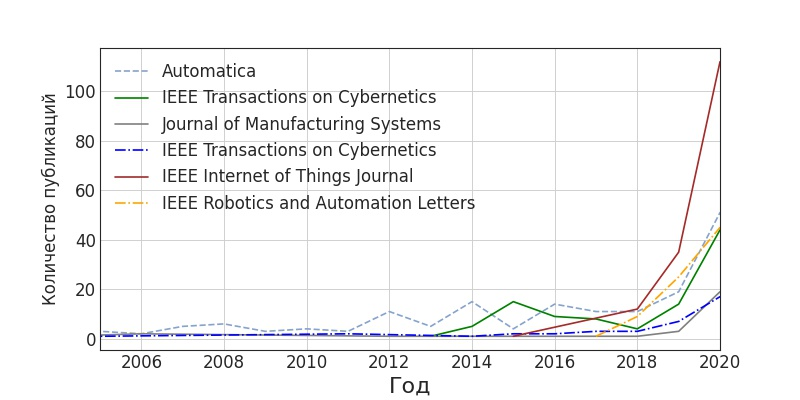
\includegraphics [scale=0.5] {my_folder/figure/schema/1.jpg}
	\caption{Тенденции количества публикаций на тему RL в специализированных журналах по управлению в технических системах} 
	\label{fig:pop-ch1}  
\end{figure}

Учитывая существующий запрос  на разработку интеллектуальных систем управление, что связано с возрастающей сложностью объектов управления, можно предполагать, что регуляторы с применением обучения с подкреплением станут неотъемлемой частью любого автоматизированного технологического процесса.
%


\section{Терминология обучения с подкреплением} \label{ch1:sec2} % ~ нужен, чтобы избавиться от висячего предлога (союза) в конце строки

Обучение с подкреплением -- это класс методов машинного обучения, которые основанны на взаимодействии алгоритма со средой и изменения стратегии действия или политики управления на основе стимулов, полученных в ответ на действия алгоритма, с целью получения желаемого результата. Цель применения методов RL — определить последовательность входных сигналов, которая обеспечивает желаемую работу динамической системы, начиная с минимальных знания о работе системы.

Агент -- интеллектуальная сущность (система/робота/алгоритм) принимающая решения, взаимодействует с объектом, который называется окружением или средой (англ., environment).  На каждом шаге последовательности $t = 0, 1, 2, ..$ агент и среда взаимодействуют. Среда или окружение задается, состоянием $S_t \in S$, где $S$ -- множество всех возможных состояний. Агенту в каждый момент времени в общем случае доступно только некоторое наблюдение (англ., observation) текущего состояния среды. На основании наблюдений состояния агент выбирает действия $A_t \in A(S_t)$, $A(S_t)$ -- множество действий, которые доступны агенту в состоянии $S_t$. Процедура выбора действий агентом называются стратегией или политикой (англ., policy) и обозначается как $\pi_t$, описывая вероятность выбора действия $A_t = a$ в состоянии $S_t = S$. По результатам применения действия $A(S_t)$ в среде, на вход агента поступает численная награда $R_{t+1} \in R$ (англ. reward) и новое состояние среды $A(S_{t+1})$. Методы RL определяют способ выбора стратегии агентом в результате полученного опыта.

Необходимо уточнить, что понимается под термином окружающая среда -- это все то, что не является агентом. На вход среды поступает действие агента, на выходе -- вознаграждение агента и состояние среды. 

\textit{Марковские процессы}. Одна из структур для RL основана на марковских процессах принятия решений (МППР). Задача RL удовлетворяет условию Марковости -- процесс зависит только от текущего состояния и не зависит от всей предыдущей истории. МППР позволяет формализовать основные элементы RL, такие как функции ценности, награды, а далее основные алгоритмы RL. Многие задачи принятия решений могут быть сформулированы как МППР, включая системы управления с обратной связью.
МППР представляет собой четверку $(S, A, P, r)$, где:

$S$ – конечное пространство состояний;

$A$ – конечное пространство действий;

$P$ – функция переходов, определяющая вероятность перейти в состояние $s'$ из состояния $s$ посредством действия $a$;

$r$  – функция награды.
При условии любого состояния $s$ и действия $a$, вероятность каждого возможного следующего состояния равна:
\begin{equation*}
p_{ij}(a, t) = P\{s_{t+1}=j|s_t=i, a_t=a\}
\end{equation*}
На рис. \ref{fig:intro} представлена общая структурная схема RL в терминах МППР.
\begin{figure}[ht!] 
	\center
	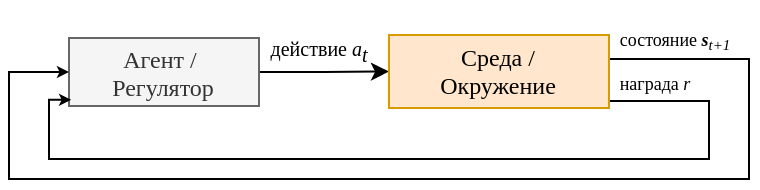
\includegraphics [scale=0.5] {my_folder/figure/schema/intro.png}
	\caption{Общая структура обучения с подкреплением} 
	\label{fig:intro}  
\end{figure}

В задаче обучения с подкреплением, цель агента формализуется в сигнале награды, которую получает агент от среды на каждом временном шаге. Использование сигнала награды для формализации цели -- одна из отличительных характеристик задачи обучения с подкреплением. Алгоритмы RL оптимизируют ту награду, которая была предоставлена ему на входе, при этом принимая истинной  <<гипотезы награды>>, которая утверждает, что любую интеллектуальную задачу можно определить (задать) при помощи функции награды. Но, как несложно догадаться, на практике дизайн функции награды оказывается сложной задачей и качество работы алгоритмы, напрямую зависит от способности формализовать цель управления.

Введено обозначение последовательности наград после временного шага $t$ -- $r_t, r_{t+1} ...$. Тогда в рамках задачи обучения с подкреплением, необходимо максимизировать ожидаемую награду $R_t$, которая равна сумме всех последующих наград. Тогда цель обучения с подкреплением, может быть сформулирована как максимизация ожидаемой награды $R_t$, которая задана как сумма всех последующих наград:
%
\begin{equation*}
R_t = r_t + r_{t+1} +  r_{t+2} + ... 
\end{equation*}
%
Такое выражение удовлетворительно для задач с конечным временным шагом,
В системах с конечным количеством шагов взаимодействия, вводится понятие разбиения взаимодействие агента и окружения на последовательности -- эпизоды. Каждый эпизод заканчивается особым терминальным состоянием, после которого осуществляется переход к заданному начальному состоянию или к выбору начального состояния из распределения начальных состояний. Среда называется эпизодичной, если для любой стратегии процесс взаимодействия гарантированно завершается не более чем за некоторое конечное число шагов.

Для ряда задач управления характерно продолжительное действие -- взаимодействие агента и окружения не разбивается на эпизоды. В этом случае ожидаемая награда, которую необходимо максимизировать, может достигать бесконечности. Для решения таких задач вводится коэффициент обесценивания (дисконтирования), тогда награда формируется следующим образом:
\begin{equation*}
R_t = r_t + \gamma r_{t+1} + \gamma^2 r_{t+2} + ... + \gamma ^{k-1} r_{t+k-1}
\end{equation*}
где $\gamma \in (0, 1]$ -- коэффициент дисконтирования.

Предполагается, что на каждом шаге с вероятностью $1-\gamma$ взаимодействие обрывается, и итоговым результатом агента станет та награда, которую он успел собрать до прерывания.Это обеспечивает приоритет получению награды в ближайшее время перед получением той же награды через некоторое время. Математически смысл дисконтирования, во-первых, в том, что данный коэффициент позволяет гарантировать ограниченность оптимизируемого функционала, а во-вторых, выполнение условий некоторых теоретических результатов, которые явно требуют $\gamma < 1$.

Учитывая терминологию приведенную выше, задача RL для заданного МППР может быть сформулирована как поиск стратегии $\pi^*$, максимизирующей среднюю дискредитированную суммарную награду. 
\begin{equation}
\label{eq:fun-ch1}
J(\pi) = E_{\pi}\sum_{t=0}^{\infty}\gamma^{t}r(s_t, \pi(s_t)) \rightarrow \max_{\pi}
\end{equation}


В основе многих алгоритмов RL лежит понятие функции ценности и функции ценности действия. Это в некотором роде <<обобщение>> функционала \ref{eq:fun-ch1}, варьируя начальное состояние. \textit{Функция ценности} (англ. Value Function) или оценочная функция состояния $V^{\pi}(s)$ показывает сколько набирает в среднем агент из состояния $s_t$ при стратегии $\pi$. Функция ценности определяется для отдельных стратеги $\pi$ и равна сумме наград:
\begin{equation}
\label{eq:val-ch1}
V^{\pi}(s) = E_{\pi}\{R_t | s_t = s\} = E_{\pi} \left[\sum_{t=0}^{\infty}\gamma^{t}r(s_t, \pi(s_t))\Bigg|s_t = s \right]
\end{equation}
где $E_{\pi}$ -- ожидаемое значение награды $R_t$ при действии агента в соответствии со стратегией $\pi$ на каждом $t$.

\textit{Функция ценности действия} $Q^{\pi}(s, a)$ (англ. Value Action) для стратегии $\pi$ характеризует сколько набирает в среднем агент из состояния $s_t$ после выполнения действия $a$. 
\begin{equation*}
Q^{\pi}(s, a) = E_{\pi}\{R_t | s_t = s, a_t = a\} = E_{\pi}\left[\sum_{t=0}^{\infty}\gamma^{t}r(s_t, \pi(s_t))\Bigg|s_t = s, a_t = a\right]
\end{equation*}

Функцию ценности и функцию ценности действий также называют V-функцией и Q-функцией, соответственно.

Исходя из задания V-фунции \eqref{eq:val-ch1} задача RL формулируется как определение политики $\pi(s,a)$, которая максимизирует награду: 
\begin{equation*}
\pi^{*}(s,a) = \underset{\pi}{\arg \max}  V_t^{\pi}(s) = \underset{\pi}{\arg \max }  E_{\pi} \left[\sum_{t=0}^{\infty}\gamma^{t}r(s_t, \pi(s_t))\Bigg|s_t = s \right]
\end{equation*}

Политика $\pi^{*}(s,a)$ называется оптимальной политикой, и соответствующее оптимальное значение V-функции задается как:
\begin{equation*}
V_t^{*}(s) = \underset{\pi}{\max }  V_t^{\pi}(s) = \underset{\pi}{\max }  E_{\pi} \left[\sum_{t=0}^{\infty}\gamma^{t}r(s_t, \pi(s_t))\Bigg|s_t = s \right]
\end{equation*}

Легко заметить, что для максимизации $V_t^{\pi}(s_0)$, где $s_0$ -- стартовое состояние, необходимо максимизировать $V_t^{\pi}(s)$. То есть задача имеет подзадачи эквивалентной структуры. Ряд методов RL основывается на рекурсивном свойстве V-функции. Тоже верно и для Q-функции. Это означает то, что для этих функций может быть записано уравнение Беллмана, которое выражает отношение между значениями функций в текущем состояний и значением в последующих состояний.
%
\section{Историческая справка}

Термин <<подкрепление>> (англ. reinforcement) унаследован из поведенческой психологии, а именно из работ физиолога И.П. Павлова. Здесь подкрепление обозначает награду или наказание за  результат, который зависит как от принятых решений так и от внешних, в общем случае, не контролируемых воздействий. Под обучением здесь понимается поиск способов достичь желаемого результата методом проб и ошибок, то есть попытки решить задачу и использовать накопленный опыта для усовершенствования своей стратегии выбора действий в будущем.

Специалисты в области обучения с подкреплением на раннем этапе истории выделяют два основных  направления развития. Одно направление связано с обучением методом проб и ошибок. И направление оптимального управления и решения задачи с применением динамического программирования.

Главной психологической идеей, которая используется в обучении с подкреплением, является метод проб и ошибок, предложенный ученым и философом Александром Бэном в 1855 году. Ученый объясняет возникновение произвольных движений -- вводит представление о спонтанной активности нервной системы. Если движение более одного раза совпадает с состоянием удовольствия, то некоторая <<сила>> устанавливает между ними связи. На базе идеи метода проб и ошибок начиная с 1930 годов было сделано ряд автоматов, демонстрирующий этот подход. Самая ранняя демонстрация — машина Томаса Росса 1933-ого года, которая могла пройти простейший лабиринт и запомнить последовательность переключателей. В 1952 году Клод Шеннон продемонстрировал лабиринт с роботом-мышью, который передвигался по лабиринту с помощью трех колес и магнита с обратной стороны лабиринта, он мог запомнить путь по лабиринту, исследуя его тем самым методом проб и ошибок. Появление таких электро-механических машин открыло путь к написанию компьютерных программ, способных к разным типам обучения, некоторые из которых были способны к обучению методом проб и ошибок.

Независимо развивался подход оптимального управления. Термин «оптимальное управление» появился в конце 1950-х годов и применялся для описания задачи проектирования устройств управления,при условии максимизации заданной характеристики поведения динамической системы во времени. Один из ключевых подходов к решению задачи оптимального управления был разработан в середине 1950-х годов Ричардом Беллманом и другими учеными путем обобщения теории Гамильтона–Якоби, созданной в XIX веке. Данный подход основан на решении функционального уравнения Беллмана, и носит название -- динамическое программирование (ДП) \cite{bellman1957dp}.  Другое ключевое понятие, как уже было сказано ранее, -- это МППР. В работе \cite{bellman1957markovian} описана дискретная стохастическая версия задачи оптимального управления, известная под названием «марковский процесс принятия решений» (МППР, англ.  MDP).  В работе Ховарда Роналда \cite{howard:dp}  предложен  метод  итерации  по стратегиям  для  МППР.  
Все это –  ключевые элементы, которые лежат в основе обучения с подкреплением. Известно, что ДП –  единственный применимый на практике способ решения общих стохастических задач оптимального управления. Большим ограничением ДП является «проклятье размерности» -- требования к вычислительной мощности растут экспоненциально с ростом числа переменных состояния.  Несмотря на ряд ограничений и недостатков, связанных с сложностями хранения больших объемов и большими вычислительными затратами на расчеты, ДП гораздо более эффективно и распространено, чем любой другой общий метод. 

Развитие оптимального управления и обучения с подкреплением происходило независимо, так как данные области ставят перед собой разные цели. 
Так же влияет тот факт, что динамическое программировании  представляется как  пакетный  метод  вычислений,  который  сильно  зависит от  наличия  точной  модели  системы  и  аналитических  решений  уравнения  Беллмана. К  тому же  простейшая  форма  динамического  программирования – вычисление,  происходящее  в  обратном  направлении  по  времени,  поэтому  трудно  понять, как  его  можно  применить в  процессе  обучения, который  по  необходимости протекает  в  прямом  направлении. 

Некоторые  из  первых  работ  по  динамическому  программированию, содержат в себе и идеи обучения например  \cite{bellman1959functional}.  В  работе  \cite{werbos1987} приводятся  явные  аргументы  в  пользу  более  тесной  связи  между  динамическим программированием  и  методами  обучения  и  доказывается,  что  динамическое программирование  имеет  прямое  отношение  к  пониманию работы  нейронов и  когнитивных  механизмов.  


Явная связь методов  динамического программирования  с  обучением для дискретных стохастических систем отражена в работе  Криса  Уоткинса  1989  года \cite{watkins1989learning},  в  которой  обучение с  подкреплением изложено  с  позиций  формализма  МППР. Методы оптимального управления и обучения с подкреплением активно  разрабатываются  многими  исследователями, в  особенности  Димитрием Бертсеркасом  и  Джоном  Цициклисом, которые  предложили  термин  «нейродинамическое  программирование»,  описывающий  комбинацию динамического  программирования  с  нейронными  сетями \cite{bertsekas1996neuro}. Еще  один  термин,  широко  употребляемый  в  настоящее  время, -–  «приближенное (адаптивное) динамическое  программирование».  



\section{Примеры применения обучения с подкреплением}
Первоначально методы RL применялись только к простым задачам, но применение глубоких нейронных сетей позволило применять RL для систем другого уровня сложности. Сейчас RL применяется в самых разных областях: робототехника, финансы, автономные транспортные средства, медицина и здравоохранения, оптимизация процессов и обнаружение неисправностей. Ниже рассмотрены основные области применения RL:
\begin{itemize}[]
	\item Промышленная робототехника -- активно развивающаяся область применения RL, поскольку является естественным внедрением этой парадигмы в практику \cite{kober2013reinforcement}.
	Например, использование глубокого обучения и обучения с подкреплением позволяет обучать роботов, способных захватывать различные объекты - даже те, которые не видны во время обучения. Или другой пример -- обучение работа повторять команды за человеком, выполняя перемещение объектов \cite{ml3}. Данные приложения могут быть использованы при сборке продуктов на сборочной линии. 
	
	
	\item Здравоохранение. RL в здравоохранении относится к методам динамического лечения (англ. Dynamic Treatment Regimes), так как алгоритмы RL позволяют находить решения для оптимального лечения пациентам в каждый момент времени. Например, вход алгоритма  -- набор клинических наблюдений и оценок пациента, выход - варианты лечения для каждого этапа.\cite{yu2019reinforcement}
	
	\item Обработка естественного языка. RL активно применяется при решении таких задач, как построение диалоговых систем \cite{li2016deep}, резюмированние и сокращение текстов \cite{paulus2017deep} машинный перевод и др.
	
	\item Проектирование архитектуры глубоких нейронных сетей. С одной стороны, применение RL для подбора архитектуры -- вычислительно затратное решение, но такой подход позволяет создавать лучшие архитектуры глубоких нейронных сетей.
	
	\item Автономные транспортные средства. Алгоритмы RL используются как для организации дорожного движения - автономные светофоры, так и для решения задач автономного вождения, например, оптимизация траектории движения, динамическое определение пути, смена полосы движения, парковка \cite{talpaert2019exploring}.
	
	\item Оптимизация производственных процессов.  RL применяется для прогнозирования технического обслуживания, диагностики оборудования режиме реального времени и управлять производственной деятельностью, а так же для оптимизации энергопотребления.\cite{waschneck2018optimization}
	Например, компания Royal Dutch Shell применяет RL в задачах по разведке и бурению. Алгоритмы RL, обученные на исторических данных бурения, а также дообученные на физических моделях, используются для управления газовыми буровыми установками при их движении по геологической среде.
\end{itemize}
%
%
\section{Классификация алгоритмов обучения с подкреплением}
В данном разделе приведена основополагающая классификация алгоритмов RL. На \firef{fig:classification-ch1} представлена лишь одна из возможных таксономий алгоритмов RL. Одна из наиболее важных классификаций основана на наличии доступа или возможность исследования агентом модели среды.\\
\begin{figure}[!h]
	\centering
	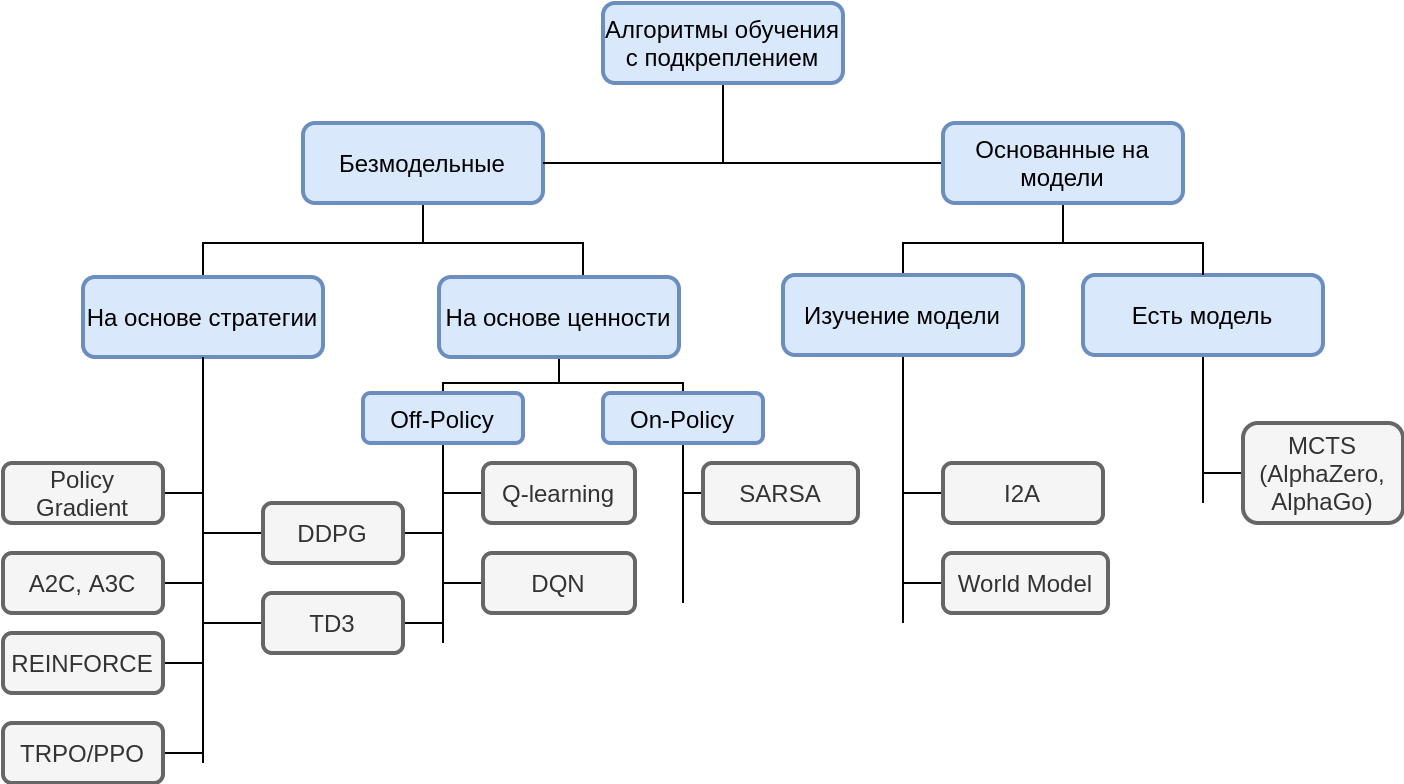
\includegraphics[width=0.7\linewidth]{my_folder/figure/schema/classification_RL.png}
	\caption{Классификация алгоритмов Rl}
	\label{fig:classification-ch1}
\end{figure}

Алгоритмы модельно-ориентированного обучения (англ. model-based RL) на первом этапе решают задачу идентификации системы либо используют уже составленную модель для решения задач управления. Безмодельное обучение (англ. model-free RL) направленно на прямой поиск управления на основе наблюдений и действий. Другими словами, безмодельные методы направлены на решение задач управления путем исследования системы и улучшения стратегий на основе прошлых вознаграждений и состояний. Модельные алгоритмы RL имеют такой же недостаток, как и классические подходы в управлении -- сложность получения достоверной модели среды (объекта).

Безмодельные методы в свою очередь делятся на два подхода: оптимизация политики  и на основе функции ценности. Алгоритмы градиента стратегии (англ. Policy-based) , использую оценки градиента функционала по параметрам политики, что означает, что каждое обновление использует данные, полученные на последней политики. Алгоритмы на основе ценности (англ. value-based) позволяют получать стратегию неявно через теорию оценочных функций. В наиболее часто встречающейся постановке для аппроксимации функции применяются глубокие нейронные сети и другие современные подходы, которые позволяют справиться с высокой дисперсией и общей неустойчивостью. 
Стоит отметить, что алгоритмы градиента стратегии применимы для сред с непрерывной областью действий, тогда как алгоритмы функций ценности применяются для дискретных систем. Поскольку такие алгоритмы используют целевую функцию основанную на уравнении Беллмана. Модельные и безмодельные алгоритмы не лишены недостатков, поэтому ведется активное развитие гибридных безмодельных алгоритмов RL.

Наколенные данные от эксперта, то есть записи взаимодействия со средой некоторой стратегии, не обязательно оптимальной, могут упростить задачу поиска условного оптимального решения ряда алгоритмов RL. Исходя из способности алгоритма использовать опыт взаимодействия со средой произвольной стратегии, выделяют on-policy и off-policy алгоритмы. Алгоритм off-policy способен использовать для обучения опыт взаимодействия произвольной стратегии. То есть появляется возможность проводить очередной шаг обучения на произвольных траекториях, сгенерированных произвольными стратегиями. Для алгоритма on-policy на очередной итерации требуется опыт взаимодействия конкретной, предоставляемой самим алгоритмом, стратегии. В то же время, накопленные данные от эксперта могут быть использованы для инициализации on-policy алгоритмов. Важно, что off-policy алгоритмы способны на данных произвольного эксперта условно сойтись к оптимуму при достаточном объёме и разнообразии экспертной информации, не требуя дополнительного взаимодействия со средой.



\section{Методы и алгоритмы обучения с подкреплением}
\label{ch1:sec6}
\textit{Динамическое программирование}. Динамическое программирование (ДП) -- один из фундаментальных модельных методов в RL, который основан на уравнении Беллмана. Базовыми алгоритмами ДП являются итерирование стратегий (англ., Policy iteration, PI)  и итерирование ценности (англ., Value iteration, VI). Алгоритм PI во время одной итерации вычисляет функцию награды для текущей стратегии, потом улучшает эту стратегию, то есть оценивание и улучшение стратегии выполняется циклически, тогда как в алгоритме VI -- оценивание и улучшение стратегии выполняется за одно обновление.
В литературе по RL процесс вычисления функции ценности состояния $V^{\pi}$ для произвольной стратегии $\pi$ называют оценкой стратегии (англ. Policy Evaluation) или задачей прогнозирования. Вычисление функции ценности необходимы для того, чтобы далее найти улучшенную стратегию управления. Процесс формирования новой, улучшающей исходную, стратегии называется улучшением стратегии (англ., Policy Improvement). Так, вычисленное значение функции ценности позволяет улучшить стратегию, в частности, жадной стратегией:
\begin{equation*}
\pi' = argmax_a Q_{\pi}(s, a) = argmax_a \sum_{s',r}p(s'|s,a)[r + \gamma V_pi(s')]
\end{equation*}

Алгоритм итерация по стратегиям представлен на \firef{fig:PI-ch1}. Алгоритм итерация по ценности представлен на  \firef{alg:VI}.
\begin{figure}[ht!]
	\begin{tcolorbox}
		\textbf{1. Инициализация} $V(s) \in \mathcal{R}$ и $\pi(s) \in \mathcal{A}(s)$ для всех $s \in \mathcal{S}$ \\
		\textbf{2. Оценка стратегии}
		Пока {$\Delta < \theta$}
		
		{$v:=V_k(s)$}
		
		{$V_{k+1}(s):=\sum_{s',r}p(s'|s,\pi(a))[r + \gamma V_k(s')]$}
		
		$\Delta := \max(\Delta, |v - V_{k+1}(s)|)$\\
		Конец цикла\\
		{\textbf{3. Улучшение стратегии}}\\
		{Стратегия устойчива:=истинно}\\
		Цикл {по $s\in\mathcal{S}$}
		
		{$b:=\pi(s)$}
		
		{$\pi(s) = argmax_a Q_{\pi}(s, a) = argmax_a \sum_{s'r}p(s'|s,a)[r + \gamma V_{k+1}(s)$]}
		
		Если {$b\neq \pi(s)$} тогда
		
		Стратегия устойчива:=ложно\\
		Конец цикла\\
		Если Стратегия устойчива тогда
		
		выход\\
		иначе переход к шагу 2
		
	\end{tcolorbox}
	\caption{Алгоритм итерирование стратегии}
	\label{fig:PI-ch1}
\end{figure}



\begin{figure}[ht!]
\begin{tcolorbox}
 \textbf{1. Инициализация} $V_0(s)$  произвольно для всех $s \in \mathcal{S}$\\ 
{\textbf{2. Оценка стратегии}}\\
Пока {$\Delta < \theta$}

{$v:=V_k(s)$}

{$V_{k+1}(s):=\sum_{s',r}p(s'|s,\pi(a))[r + \gamma V_k(s')]$}

$\Delta := \max(\Delta, |v - V_{k+1}(s)|)$\\
Конец цикла\\
{\textbf{3. Улучшение стратегии}}\\
{$\pi(s) = argmax_a \sum_{s'r}p(s'|s,a)[r + \gamma V_{k+1}(s)]$}\\

\end{tcolorbox}
	\caption{Алгоритм итерирование ценности}
	\label{alg:VI}
\end{figure}
%

%Асинхронное динамическое программирование
Недостатком методов ДП является то, что они требуют вычислений в каждом состоянии. В случае, если множество состояний велико, это может потребовать больших вычислительных ресурсов.
Асинхронные алгоритмы ДП обновляют оценки значений только подмножества состояний, а не всего набора на каждой итерации оценки политики. Такие алгоритмы обновляют значения состояний в любом порядке, используя значения других доступных состояний.
Как было сказано ранее, схема алгоритма PI состоит из двух чередующихся взаимодействующих шагов: оценка и улучшение стратегии. Шаг оценки стратегии устанавливает связь функции ценности с текущей стратегией. Шаг улучшения стратегии делает стратегию жадной к текущей функции ценности. В алгоритме VI между двумя улучшениями стратегии только одна итерация оценивания стратегии. В асинхронных методах ДП процесс оценивания и улучшение стратегии разбивается на более крупные чередующиеся итерации.

Одни из главных недостатков ДП -- экспоненциальное возрастание сложности вычислений с увеличением числа состояний (<<Проклятье размерности>>) и необходимость модели объекта. Несмотря на это, идеи оценки стратегии и итерирования по стратегии лежат в основе почти всех алгоритмов ОП.

В отличии от ДП методы Монте-Карло (МК) не предполагают полного знания о модели. Такие методы предполагают наличие данных -- набор состояний, действий и наград, полученных при взаимодействии с средой. Для применения методов МК требуется, чтобы задача была эпизодическая, так как методы МК инкрементны на уровне эпизодов, а не на уровне шагов. В отличии от ДП оценка для каждого состояния в методах МК -- независимы.
Подробно не будет останавливаться на методах МК и ДП.
%
%

\textit{Обучение на основе временных различий}.
Обучение на основе временных различий (англ., Temporal Difference, TD) или TD-обучение -- это метод обучения с подкреплением без использования моделей, где агент обучается на каждом отдельном действии, которое он предпринимает и при этом обновляет знания агента на каждом временном шаге (действии), а не в каждом эпизоде.TD-методы совмещают в себе идеи методов МК и ДП. Коррекция в простейшем TD-методе производится путем улучшения ценности на небольшую величину в направлении оптимального значения:
\begin{equation*}
\label{td_function}
V(s_t) = V(s_t) + \alpha[r + \gamma V(s_{t+1}) - V(s_t)]
\end{equation*}
где $\alpha$ -- параметр, который определяет степень изменения ценности состояния при каждом обновлении. Если $a = 0$, то ценность состояния не изменяется. Если же $a = 1,$ то ценность состояния будет равна $r + \gamma V(s_{t+1})$ -- старая ценность затирается. К алгоритмам TD-методов относятся: Q-learning, SARSA, R-learning, методы исполнитель-критик

На рис.\ref{fig:q_learn-ch1} -- \ref{fig:sarsa-ch1} представлены алгоритмы Q-learning, SARSA. Алгоритм Q-learning -- это табличный безмодельный off-policy алгоритм RL. Это метод основан на временных разностей для вычисления оптимальной Q-функции с $\varepsilon-$жадной стратегией исследования, то есть агент выбирает случайное действие с вероятностью $\epsilon$, но использует известное лучшее действие. Алгоритм наследует от TD-обучения характеристики одношагового обучения, такие как возможность обучаться на каждом шаге и способность обучаться на опыте, не имея модели окружающей среды.
Q-learning отличается от SARSA прежде всего тем, что это алгоритм с разделенной стратегией. Разделенная стратегия означает, что обновление производится независимо от того, какая стратегия использовалась для накопления опыта, то есть алгоритмы с разделенной стратегией
могут использовать прежний опыт для улучшения стратегии. Стратегия, которая применяется для улучшение стратегии -- целевая, а стратегия для взаимодействия с окружающей средой -- поведенческая.
Алгоритм состоит из следующих шагов: 1. Инициализация Q-таблицы с нулевыми значениями, то есть в начальный момент времени все стратегии равновероятны и равноценны. 2. Выбор действия с наибольшей ценностью. 3. Отправка на вход среды выбранного действие, на выходе получаем вознаграждение. 4. Обновление Q-таблицы с учетом полученного вознаграждения.
Гиперпараметрами алгоритма являются $\alpha \in (0,1] $ -- параметр экспоненциального сглаживания, $\varepsilon > 0 $ -- параметр исследования.

	\begin{figure}[ht!]
		\centering
		\begin{tcolorbox}
\textbf{Инициализация} $Q(s, a)$ произвольно для всех $s \in \mathcal{S}$, $\alpha \in \mathcal{A}$\\
\textbf{Цикл} {по эпизодам}

\textbf{Инициализация} $s$

Цикл {по шагам эпизодов $k$}

\textbf{Выбор} $a_k$: с вероятностью $\epsilon$ принимаем $a_k \sim Uniform(\mathcal{A})$

 иначе $a_k = argmax Q(s_k, a_k)$
			
\textbf{Выполнение} действие $a_k$

\textbf{Нахождение} $r_k, s_{k+1}$

\textbf{Обновление} 

$Q(s,a ) \leftarrow Q(s, a) + \alpha [r_k + \gamma \max_{a_{k+1}}Q(s_{k+1}, a_{k+1})-Q(s_k,a_k)]$

\textbf{Конец цикла}\\
\textbf{Конец цикла}
		\end{tcolorbox}
		\caption{Алгоритм Q-learning}
		\label{fig:q_learn-ch1}
\end{figure}
%
\begin{figure}[!ht]
		\centering
		\begin{tcolorbox}%ht
\textbf{Инициализация} $Q(s, a)$ произвольно для всех $s \in \mathcal{S}$, $\alpha \in \mathcal{A}$\\
\textbf{Цикл} {по эпизодам}

\textbf{Считывание} $s_0$, находим $a_k \sim Uniform(\mathcal{A})$

\textbf{Цикл} {по шагам эпизодов $k$}

\textbf{Нахождение} $r_k, s_{k+1}$

\textbf{Выбор} $a_{k+1}$: с вероятностью $\epsilon$ принимаем $a_{k+1} \sim Uniform(\mathcal{A})$

иначе $a_{k+1} = argmax Q(s_{k+1}, a_{k+1})$
			
\textbf{Выполненине} действия $a_k$
			
\textbf{Обновление} 
$Q(s,a ) \leftarrow Q(s, a) + \alpha [r_k + \gamma Q(s_{k+1}, a_{k+1})-Q(s_k,a_k)]$

\textbf{Конец цикла}\\
\textbf{Конец цикла}
		\end{tcolorbox}
		\caption{Алгоритм SARSA}
		\label{fig:sarsa-ch1}
	\end{figure}

Разница между этими двумя алгоритмами в том, что SARSA выбирает действие, соответствующее той же текущей политике, и обновляет его Q-значения, тогда как Q-обучение выбирает жадное действие, то есть действие, которое дает максимальное значение Q для состояния, то есть оно следует оптимальной политике.

\textit{Аппроксимация V-функции}.

Главным недостатком перечисленных выше методов является необходимость хранить в памяти большие объемы данных при увеличении сложности объекта, а так же сложность работы с непрерывным пространством действий. Необходимо ввести аппроксимацию V-функции (Q-функции), что позволит представить функцию в  ограниченной области определения, располагая памятью фиксированного объема.Применение аппроксимации функций позволяет заменить
пространство состояний набором признаков, порождаемых по исходным со-
стояниям

Основная идея аппроксимации функций – воспользоваться набором при-
знаков для оценки значений V-функции (Q-функции). Есть несколько способов отобразить признаки на значения функции, например линейная аппроксимация, решающие деревья, алгоритм ближайших соседей, искусственные нейронные сети. В  случайно линейной аппроксимации функция ценности состояний записывается в виде взвешенной суммы признаков. Как можно ожидать, нейронные сети используются чаще других подходов. В частности, используются глубокие	нейронные сети (ГНС). 




%\begin{table} [htbp]% Пример оформления таблицы
%	\centering\small
%	\caption{Представление данных для сквозного примера по ВКР \cite{Peskov2004}}%
%	\label{tab:ToyCompare}		
%		\begin{tabular}{|l|l|l|l|l|l|}
%			\hline
%			$G$&$m_1$&$m_2$&$m_3$&$m_4$&$K$\\
%			\hline
%			$g_1$&0&1&1&0&1\\ \hline
%			$g_2$&1&2&0&1&1\\ \hline
%			$g_3$&0&1&0&1&1\\ \hline
%			$g_4$&1&2&1&0&2\\ \hline
%			$g_5$&1&1&0&1&2\\ \hline
%			$g_6$&1&1&1&2&2\\ \hline		
%		\end{tabular}	
%	\normalsize% возвращаем шрифт к нормальному
%\end{table}


% \firef{} от figure reference
% \taref{} от table reference
% \eqref{} от equation reference


%\FloatBarrier % заставить рисунки и другие подвижные (float) элементы остановиться

%\section{Выводы} \label{ch1:conclusion}



Вывод по главе \thechapter. В ходе анализа и изучения области обучения с подкреплением, сделаны следующие выводы:
\begin{itemize}

	\item МППР -- нотация для представления задачи обучения с подкреплением;
	\item Функция ценности и функция ценности действия -- основополагающие термины для дальнейших исследований; 
	\item Динамическое программирование рассматривается как один из главных способов обучения агента;
	\item Область управления и область обучения с подкреплением связаны математической базой, а именно уравнение Беллмана;
	\item Применение методов обучения с подкреплением распространено в области рекомендательных систем и игр;
\end{itemize}


%% Вспомогательные команды - Additional commands
%
%\newpage % принудительное начало с новой страницы, использовать только в конце раздела
%\clearpage % осуществляется пакетом <<placeins>> в пределах секций
%\newpage\leavevmode\thispagestyle{empty}\newpage % 100 % начало новой страницы	         	 % Глава 1
\ContinueChapterBegin % размещать главы <<подряд>> 
\newpage
\chapter{Методы обучения с подкреплением в задаче управления} \label{ch2}
	
% не рекомендуется использовать отдельную section <<введение>> после лета 2020 года
%\section{Введение} \label{ch2:intro}

 
Обучение с подкреплением предлагает мощные алгоритмы разработки оптимального управления для систем с нелинейностями, со сложной неизвестной стохастической динамикой. Данная глава охватывает подходы RL с точки зрения инженера по управлению. В этой главе приводятся объяснения, как аппроксимация позволяет использовать RL с непрерывными состояниями и управляющими воздействиями.
Цель данной главы -- преодоление рассогласованности терминологии управления и RL.


\section{Переход между нотациями} \label{ch2:title-abbr} %название по-русски

Анализ динамических систем с использованием механики Лагранжа, Гамильтона, позволяет получить описание системы в форме нелинейных ОДУ или разностных уравнений. В первом случае объект управления описывается уравнением вида: 
\begin{equation*}
	\dot x = f(x, u),
\end{equation*}
где  $x(t) \in X \subseteq R^n$, $u(t) \in U \subseteq R^m$ -- управление.

Показатель качества (критерий оптимальности), по которому проектируется система управления, задается в виде:
\begin{equation*}
	J=\int_{0}^{t_f} L(t, x(t), u(t))dt + h(x(t_f), t_f),
\end{equation*}
где $t_f$ -- конечное время.

Такое представление системы, в отличии от МППР, имеет непрерывное пространство состояний, непрерывный вход, а так же непрерывность во времени. 

Во втором случае система либо дискретна по своей природе, либо приводится к дискретной форме: 
\begin{equation*}
x_{k+1} = f(x_k, u_k), \space  k=0, 1,.., N,
\end{equation*}

При этом выполняется свойство марковости, так как состояние в момент времени $k+1$ зависит только от состояния и входов в момент времени $k$. При этом $x_k$ и $u_k$ могут принадлежать конечному или счетному множеству, а так же континууму.
Показатель качества для дискретных систем имеет вид:
\begin{equation}
\label{eq:J_cost}
J = g_N(x_N) + \sum_{k=0}^{N-1} g_k(x_k, u_k),
\end{equation}
где \(g_N(x_N)\) -- терминальные (конечные) значения, N  -- число временных шагов (этапов, стадий)

В некоторых задачах важно получить представление об оптимальном процессе при длительном, практически неограниченном процессе. Отдельно выделяют задачи оптимального управления с бесконечным временем, когда $t_f\xrightarrow{}\infty$ или $N \xrightarrow{} \infty$. Особенность таких задач связана с тем, что показатель качества представляет собой бесконечную сумму или несобственный интеграл. 
Одни из наиболее распространенных подходов для задач с бесконечным временем является введение дисконтирования:
\begin{equation*}
	J = \int_{0}^{\infty} L(x(t), u(t))dt
\end{equation*}
или в дискретном случае:
\begin{equation*}
	J = \sum_{k=0}^{\infty} \gamma^{k}r(x_k,u_k)
\end{equation*}
где $0 < \gamma \leq 1$ - коэффициент дисконтирования.
Введение коэффициента дисконтирования гарантирует сходимость ряда или интеграла в большинстве случаев. Физический смысл — штраф или награда в будущем имеют меньшую значимость, чем текущая. Кроме того, введение дисконтирования уменьшает влияние неточности модели на показатель качества.

Рассмотрим переход от разностных уравнений к МППР и обратно. Пусть задан МППР:
\begin{equation*}
	p_{ij}(u,k)= P\{x_{k+1} = j |x_k = i, u_k = u\}
\end{equation*}
Соответствующая дискретная система будет $s_{k+1} = w_k$, где 
\begin{equation*}
{P\{w_k = j |x_k = i, u_k = u\} = p_{ij}(u_k)}
\end{equation*}
В обратную сторону, пусть задана дискретная система:
\begin{equation}
x_{k+1} = f(x_k, u_k, w_k)
\end{equation}
где $w_k \sim P_k(w_k|x_k,u_k)$ -- известно. Тогда
\begin{equation}
p_{ij}(u,k)= P_k\{W_k(i, u, j) |x_k = i, u_k = u\}
\end{equation}
где $W_k(i, u, j) = {w|j = f_k(i, u, w)}$

Как видно, в обучении с подкреплением обычно в общем случае рассматриваются стохастические системы, однако, для простоты, в данной работе ограничимся рассмотрением только детерминированных систем.

\section{Обучение с подкреплением для дискретных систем}

\textit{Классическое динамическое программирование}. Все задачи ДП направлены на работу динамических систем с дискретным временем. В детерминированных системах \(x_{k+1}\) определено. 
Задача ДП рассматривает динамические системы с дискретным временем вида:
\begin{equation}
x_{k+1} = f_k(x_k, u_k),
\end{equation}
где $k=0, 1,.., N-1$.

Цель -- найти управление, минимизирующее показатель качества:
\begin{equation}
\label{eq:J_cost}
J(x_0;u_0,...,u_{N-1}) = g_N(x_N) + \sum_{k=0}^{N-1} g_k(x_k, u_k),
\end{equation}
Тогда оптимальное значение функционала записывается как:
%
\begin{equation}
\label{eq:J_cost_min}
J^*(x_0) = \min_{\substack{u_k \in U_k(x_k) \\ k=0,...,N-1}} J(x_0;u_0,...,u_{N-1}),
\end{equation}

При решении задачи \eqref{eq:J_cost_min} методом ДП, поиск последовательности $J^*_N(x_N), J^*_{N-1}(x_{N-1}),..., J^*_0(x_0)$ осуществляется следующим образом:
\begin{equation*}
	J^*_N(x_N) = g_N(x_N) \text{ для всех }x_N
\end{equation*}
\begin{equation*}
	J^*_k(x_k) = \min_{u_k \in A_k(x_k)} [g_k(x_k, u_k) + J^*_{k+1}(f_k(x_k, u_k))] \text{ для всех } x_k
\end{equation*}

После этого, зная $J^*_{N}(x_{N}), J^*_{N-1}(x_{N-1})..., J^*(x)$, можно последовательно найти $u_0, ..., u_{N-1}$:


\begin{equation*}
	u^{*}_k \in \underset{u_k \in U_k(x^*_k)}{\arg \min}[g_0(a^*_k, x_k) + J^*_{k+1}(f_k(x^*_k, u_k))],
\end{equation*}
\begin{equation*}
	x^*_{k+1} = f_k(x^*_k, u^*_k),
\end{equation*}

Таким образом, для нахождения $u_0, ..., u_{N-1}$ необходимо вычисление всех $J^*_k(x_k)$. На практике вычисление \(J^*_k\) с помощью ДП занимает большое количество времени, поскольку количество \(x_k\) и \(k\) может быть очень большим. Главным недостатком метода является «проклятие размерности» –- сложность вычислений возрастает с увеличением размерности задачи. Помимо этого формирование управляющего воздействия методом ДП протекает не в режиме реального времени (режим off-line). С ростом сложности системы возникает необходимость хранения огромного количества данных, увеличение доли шумов. Решение задачи оптимального управления методом ДП, предполагает знание модели объекта, в следствии чего качество регулятора зависит напрямую от качества построения математической модели объекта. Отсутствие универсального алгоритма, который был бы пригоден для решения всех задач рассматриваемого класса. Алгоритмы ДП объединены общей идеей, но в каждом конкретном случае должны формироваться применительно к специфике прикладной задачи, поэтому отсутствие универсального алгоритма -- еще один недостаток методов оптимального управления, таких как ДП.


\section{Бесконечное время и методы}
Рассмотрим стационарную систему $x_{k+1} = f(x_k, u_k)$ на бесконечном интервале времени:
\begin{equation}
\label{f: fun_inf}
J = \sum_{k=0}^\infty g(x_k, u_k)
\end{equation}

Необходимо найти закон управления $\mu (x)$, который является также стационарным, что значительно упрощает синтез и реализацию. С другой стороны, в случае рассмотрения систем на бесконечном интервале времени мы не можем итеративно двигаться назад, начиная с терминального состояния, как мы это делали в случае конечного времени.
Обозначим как $J_{\mu} (x_0)$ значение функционала при законе управления $\mu$ и начальном условии $x_0$ . Тогда:
\begin{equation*}
	J_{\mu}(x_k) = \sum_{t=k}^{\infty} g(x_t, \mu(x_t)) = g(x_k,\mu(x_k)) + J_\mu(x_{k+1}), \space J_{\mu}(0) = 0
\end{equation*}
произведена замена бесконечного суммирования в \ref{f: fun_inf} на решение разностного уравнения. Отсюда можно получить следующий алгоритм решения рассматриваемой задачи, называемый итерации по ценности (VI):
\begin{equation*}
	\begin{matrix}
		J_0(x) = 0 \\
		J^*_{k+1}(x) = \underset{u_k \in U(x)}{\min}{[g_k(x_k, u_k) + J^*_{k}(f_k(x_k, u_k))]}, \space k = 0, 1, ...
	\end{matrix}
\end{equation*}

Рассмотренный выше алгоритм для конечного случая — тоже VI. Тот же самый алгоритм, переписанный в более привычном для RL виде:

Итерация по ценности:
\begin{enumerate}[1.]
	\item Инициализация. Выбор произвольного закона управления $\mu_0(x)$, $k=0$ и $J_0(s)$
	\item Шаг policy evaluation (оценка политики).
	\begin{equation*}
		J_{k+1}(x):=g(x, \mu_k(x)) + J_k(f(x,u))
	\end{equation*}
	
	\item Шаг policy improvement (обновление политики). Обновление закона управления
	\begin{equation*}
		\mu_{k+1}(x) =  \underset{\mu(\cdot)}{\arg\min}(g(x, \mu_k(x)) + J_{k+1}(f(x,u)))
	\end{equation*}
\end{enumerate}

Другой алгоритм -- итерация стратегии (PI):

\begin{enumerate}[1.]
	\item Инициализация. Выбор произвольного закона управления $\mu_0(x)$, $k=0$ и $J_0(s)$
	\item Шаг policy evaluation (оценка политики).
	\begin{equation*}
		J_{\mu_{k+1}}(x)=g(x, \mu_k(x)) + J(f(x,\mu_k(x)))
	\end{equation*}
	
	\item Шаг policy improvement (обновление политики). Обновление закона управления
	\begin{equation*}
		\mu_{k+1}(x) =  \underset{\mu(\cdot)}{\arg\min}(g(x, \mu_k(x)) + J(f(x,\mu_k(x))))
	\end{equation*}
\end{enumerate}
%\textbf{Про разницу между ними, про GPI, про всякие сходимости}




Рассмотрим вариант PI алгоритма, в котором шаг оценки стратегии производится неточно, в частности, алгоритм начинается с некоторого $J_0$ и генерирует последовательность пар функций стоимости и закона управления ${J_k, \mu_k}$ следующим образом: учитывая $J_k$, мы генерируем $\mu_k$ в соответствии с:
\begin{equation*}
	\mu_{k}(x) =  \underset{\mu(\cdot)}{\arg\min}(g(x, u) + J_{k}(f(x,u)))
\end{equation*}
и тогда получаем $J_{k+1}$ при $m_k \geq 1$
\begin{equation*}
		J_{\mu_{k+1}}(x_0)=J_k(x_{m_k}) + \sum^{m_k-1}_{t=0}g(x_t,\mu_k(x_t)))
\end{equation*}
где ${x_t}$ -- последовательность, сгенерированная с использованием $\mu_k$ и начиная с $x_0$, $m_k$ - произвольные положительные целые числа. При $m_k = 1$ алгоритм эквивалентен  алгоритму VI, а частный случай $m_k = \infty$ -- алгоритму PI. Такой алгоритм в RL называется Обобщенная итерация стратегий (Generalized Policy Iteration, GPI) -- одна итерация решения m-шагового уравнения Беллмана чередуется с шагом обновления политики). Алгоритм GPI при любом $m$ сходится к оптимальной стратегии и оптимальной оценочной функции.

\section{Приближенное динамическое программирование}
Эти методы широко распространены под названием приближенное или адаптивное динамическое программирование \cite{werbos1992approximate} или нейродинамическое программирование \cite{bertsekas1996neuro}.

Для преодоления  проклятия размерности применяют различные аппроксимации. Аппроксимировать можно $J_k^*$ (аппроксимация in value space) и или непосредственно управление (аппроксимация in policy space). Здесь важно привести еще одну важную классификацию в зависимости от то, когда вычисляется управление: оффлайн — вычисление управления производится до начала процесса управления, онлайн — вычисляем управление непосредственно в процессе эксплуатации. Так, аппроксимация in policy space — оффлайн метод, аппроксимация in value space — в основном онлайн метод.

В случае аппроксимации <<in policy space>> мы ищем управление из заданного параметрически семейства $\mu_k(x_k, r_k)$, где $r_k$ – параметры. Если осуществили аппроксимацию, то управление легко посчитать: $u_k = \widetilde{\mu}_k (x_k , r_k )$, то есть такой подход можно использовать для аппроксимации известного закона с целью удобного онлайн использования. В общем случае собираются пары $(x^s_k , u^s_k )$, $s = 1,..., q$, такие что u $s_k$ — хорошее управление для данного $x^s_k$ . Далее определяются параметры, например, методом наименьших квадратов.


В случае аппроксимации <<in value space>> аппроксимируем $J_k^*$  функцией
$\widetilde{J}_k$ . Тогда управление находится алгоритмом ДП, минимизируя функционал на конечном горизонте плюс аппроксимация оптимальной будущей стоимости $\widetilde{J}$. Значение $\widetilde{J}$  может быть получено разными способами: симуляция методами Монте-Карло, эвристики и др.

Методы нахождения $\widetilde{J}_k$ можно условно классифицировать на 4 группы:

\begin{enumerate}[1.]
	\item \textit{Аппроксимация задачи}. Нахождение функции $\widetilde{J}_k$ в более простой задаче. Вводится ряд допущений -- уменьшение размера пространста состояния, не учитываются нелинейности и т.д. Частный случай -- агрегация;
	\item \textit{Приближенная онлайн оптимизация}. Здесь применяются окононные алгоритмы: (Алгоритм Rollout algorithms, Model Predictive Control и т.д);
	\item \textit{Параметрическая аппроксимация}. Параметризуем $\widetilde{J}_k(x_k, r_k)$ некоторой параметрической функцией, где параметры определены используя данные и, например, нейронные сети;
	\item \textit{Агрегация}. Эта группа методов обычно предполагает разбиение пространства состояний. Более того, агрегация может применяться вместе с методами (1-3) и служить начальным приближением для решения задачи другим методом.
\end{enumerate}

В данной работе остановимся на 2 и 3 подходе.


\textit{Приближенная онлайн оптимизация, метод MPC}

Идея метод состоит в том, чтобы не параметризовать политику управления параметрами $W$ (как это будет далее показано в RL), а вместо этого оптимизировать входные данные управления $u_k$ непосредственно на конечном горизонте $T$. Чтобы учесть усеченный горизонт, мы можем использовать функцию ценности при некотором законе управлении, чтобы чтобы приблизить стоимость за пределами T шагов. Таким образом, политика управления определяется выражением
\begin{equation*}
	\mu_(x_k) = \underset{\mu(\cdot)}{\arg\min}(g(x_k, u)  + J(f(x,\mu_k(x))))
\end{equation*}

Модельное прогнозирующее управление (англ. model predictive control, MPC) -- метод управления который позволяет расчитывать управляющее воздействия на основе  математической модели объекта, прогнозируя значения переменных состояния и выхода, решая задачи оптимизации в реальном времени, при этом учитывая ограничения (\firef{fig:mpc-ch2}). Регулятор минимизирует ошибку между предсказанным и фактическим значением по горизонту управления. В отличии от классических подходов управления MPC позволяет управлять близко к ограничениям, что ведет к более устойчивой работе.

\begin{figure}[ht!] 
	\centering
	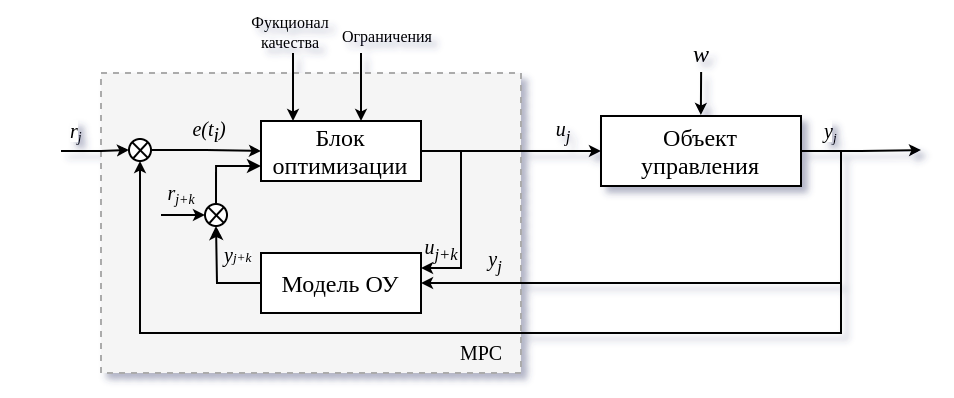
\includegraphics[width=0.9\linewidth]{my_folder/figure/schema/MPC.png}
	\caption{Структурная схема системы управления с прогнозирующими моделями}
	\label{fig:mpc-ch2}
\end{figure}


Регулятора на основе MPC получили широкое распространение в силу развития вычислительных мощностей. Отметим ключевые моменты, которые отличают подход MPC и RL: а) Так как на каждом шаге решается задача оптимизации, качества управления во многом будет зависеть от точности модель процесса. В то время как регуляторы RL не требуют какого-либо предварительного доступа к модели процесса: б) Промышленные системы управления подвержены эксплуатационным ограничениям, которые должны всегда соблюдаться. MPC устраняет эти ограничения, явно включая их в задачу оптимизации, решаемую на каждом этапе. В контроллере RL ограничения могут быть встроены непосредственно в функцию перенастройки или реализованы посредством отсечения градиента. Второй подход более мягкий -- нарушение ограничения может произойти во время обучения, но оно не приветствуется из-за огромного штрафа в сигнале вознаграждения. Надежные механизмы для безопасной работы полностью обученной системы и, действительно, для безопасной работы во время онлайн-обучения, являются открытой задачей для RL регулирования.
в) Адаптация: со временем меняются параметры систем. Поддержание производительности требует реагирования как на изменения, так и на неизвестные нарушения. Традиционные системы на основе MPC включают механизмы для
выявление несоответствия модели и объекта, но изменение параметров будет сопровождаться повторной идентификацией модели процесса. Этот процесс, который требует одновременной оценки состояния и параметров, может быть сложным и дорогостоящим. Некоторые недавние варианты MPC, такие как робастный MPC и стохастический MPC, учитывают неопределенности модели, встраивая их непосредственно в задача оптимизации. Регуляторы на основе RL автоматически корректируют параметры в сетях актеров и исполнителях. Это обеспечивает регулятор RL свойством самонастройки, так что процесс остается субоптимальным по отношению к выбранному критерию вознаграждения.



Рассмотрим \textit{параметрическую аппроксимацию}. Для этого представим оценку функции стоимости в следующем виде:
\begin{equation*}
	\label{f:approx_val_funt}
	\widetilde{J}_\mu(x) = W^T\varphi(x)
\end{equation*}
где базисный вектор $\varphi(x) = [\varphi_1(x), \varphi_2(x), ... \varphi_L(x)]$, $W \in \mathrm{R}^L$ --вектор настраиваемых параметров. Для наивной настройки весов W
требуется для каждого $x_k$ вычислять $\widetilde{J}_\mu(k)$, то есть вычисления производятся оффлайн. Для устранения этого недостатка вводится понятие временного различия (англ, Temporal Differences, TD):
\begin{equation*}
	e_k = g(x_k,\mu(x_k)) + J_{\mu}(x_{k+1}) - J_{\mu}(x_k)
\end{equation*}

Если $e_k = 0$ для всех $x_k$ , то это просто уравнение Беллмана. TD ошибка представляет собой ошибку между предсказанной и действительной наградой за действие. Это равенство должно выполняться для всех $x_k$ в любой
момент времени $k$, поэтому можно записать онлайн версии рассмотренных ранее алгоритмов.

\textit{Онлайн алгоритм итерации по стратегии (онлайн PI)}

\begin{enumerate} [1.]
	\item \textit{Инициализация}. Выбор любого допустимого закона управления $\mu_0(x_k)$
	\item \textit{Шаг оценки стратегии}. Оценка параметров $W_{j+1}$:
	\begin{equation*}
		\label{f:policy_iteration_online}
		W^T_{j+1}(\varphi(x_k) - \gamma \varphi(x_{k+1})) = r(x_k, h_j(x_k))
	\end{equation*}
	\item  \textit{Шаг улучшения стратегии}. Обновление закона управления:
	\begin{equation*}
		\mu_{j+1}(x_k) = \underset{\mu(\cdot)}{\arg\min}(g(x_k, \mu(x_k)) + W^T_{j+1}\varphi(x_{k+1}))
	\end{equation*}
\end{enumerate}


\textit{Онлайн алгоритм итерации по ценности. (онлайн VI)}
\begin{enumerate} [1.]
	\item \textit{Инициализация}. Выбор любого закона управления $\mu_0(x_k)$, не обязательно допустимой.
	\item  \textit{Шаг оценки стратегии}. Оценка параметров $W_{j+1}$:
	\begin{equation}
	\label{f:value_iteration_online}
	W^T_{j+1}\varphi(x_k) =g(x_k, \mu_j(x_k)) + W^T_{j}\gamma \varphi(x_{k+1})
	\end{equation}
	\item  \textit{Шаг улучшения стратегии}. Обновление закона управления:
	\begin{equation*}
		\mu_{j+1}(x_k) = \underset{\mu(\cdot)}{\arg\min}(g(x_k, \mu(x_k)) + W^T_{j+1}\varphi(x_{k+1}))
	\end{equation*}
\end{enumerate}

В обоих алгоритмах на шаге policy evaluation, параметры $W_{j + 1}$ можно искать методом наименьших квадратов. Однако для этого требуется обновление закона управления производить не раньше, чем через $L$ шагов с этим законом. Так как $W_{j + 1} \in R^L$ , нужно не менее $L$ уравнений для оценки этого вектора. В момент времени $x_{k+1}$ имеем набор $(x_k , \mu_(x_k), x_{k+1} , g(x_k , \mu(x_K)))$, то есть одно уравнение. Однако обычно вектор параметров $W_{j + 1}$ ищут рекурсивным методом наименьших квадратов или градиентным спуском до сходимости, а затем обновляют закон управления.

На шаге обновления закона управления необходимо осуществлять поиск функции, что плохо, поэтому необходимо параметризовать. Параметризовав шаг 3,получаем схему исполнитель-критик.

Часто реализация обучения с подкреплением осуществляется с использованием двух НС: одна в качестве критика, а другая в качестве исполнителя (рисунок 1). В этой системе управления критик и исполнитель настраиваются в режиме онлайн с использованием наблюдаемых данных. Критик и исполнитель настраиваются последовательно -- веса одной НС остаются постоянными, а веса другой настраиваются до сходимости. Эта процедура повторяется до тех пор, пока обе НС не сойдутся. Затем регулятор определяет оптимальное значение управления в режиме онлайн. Таким образом,
это онлайн оптимально-адаптивная система управления, в которой параметры аппроксимированного функционала настраиваются онлайн, обеспечивая сходимость к оптимальному управлению.
%
\begin{figure}[ht!] 
	\centering
	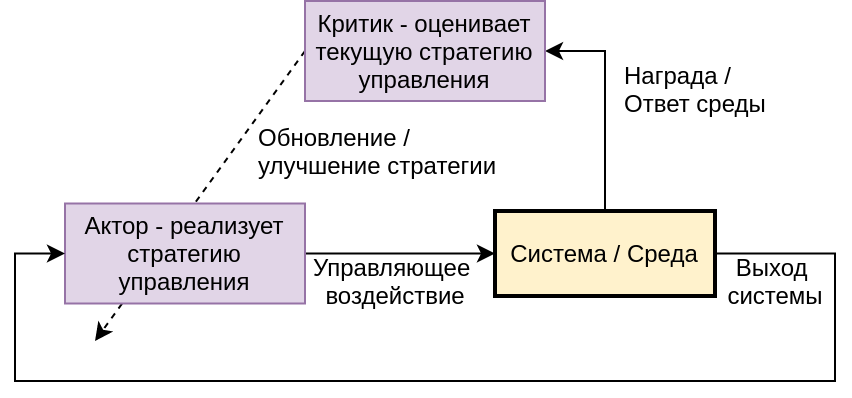
\includegraphics[width=0.8\linewidth]{my_folder/figure/schema/actor_critic.png}
	\caption{Структурная схема системы управления с прогнозирующими моделями}
	\label{fig:my_label}
\end{figure}
%
%
\section{Q-фактор}
На данном этапе получили онлайн версии с параметризацией, но в описанных выше алгоритмах, даже если мы знаем $J$, требуется знать функцию $x_{k+1} = (x_k, u_k)$. То есть все еще требуется построение модели. Поэтому вводим понятие Q-фактора.

Можно ввести следующее обозначение:
\begin{equation*}
	Q^*_k(x_k, u_k)= g_k(x_k, u_k) + J^*_{k+1}(f_k(x_k, u_k))
\end{equation*}
Тогда
\begin{equation*}
	u_k^* \in \underset{u_k \in U_k(x_k^*)}{\arg \min}Q^*_k(x_k^*, u_k)
\end{equation*}

Оптимальная стоимость записфвается как:
\begin{equation*}
	J_k^*(x_k) = \underset{u_k \in U_k(x_k^*}{\min}Q^*_k(x_k, u_k)
\end{equation*}

Тогда алгоритм ДП можно переписать через Q-фактор:
\begin{equation*}
	Q_k^*(x_k, u_k) = g_k(x_k, u_k) + \underset{u_{k+1} \in U_{k+1}(f_k(x_k, u_k))}{\min}Q^*_{k+1}(f_k(x_k, u_k), u_{k+1})
\end{equation*}

$J$ имеет преимущество, что если система меняется, то работает (online replanning).





Оптимальные методы управления обычно направлены на поиск закона управления в автономном режиме при условии наличия базовых динамических моделей. Когда лежащие в основе модели недоступны или известны только частично, используются подходы адаптивного управления в онлайн режиме \cite{landau2011adaptive}. Таким образом, можно сказать, что онлайн-методы RL -- это методы адаптивного оптимального управления. Так как RL направлено на поиск оптимального (субоптимального) закона управления в режиме онлайн с использованием измерений в реальном времени без знания модели системы.

Анализ устойчивости оптимальных и адаптивных методов управления имеет решающее значение в потенциально опасных приложениях, например, при взаимодействии человека и робота, автономная робототехника или управление электростанциями. При разработке оптимальных и адаптивных законов управления на первом этапе выбираются детерминированные настройки.
Впоследствии, потенциальные неопределенности (шумы и возмущения) которые не учтены в детерминированной настройке, исследуются с использованием различных инструментов устойчивости, чтобы сделать вывод об устойчивости, например, о локальной, асимптотической, экспоненциальной устойчивости.

В отличие от стандартных подходов в управлении, которые с самого начала ставят требования полной устойчивости, подходы RL требуют дополнительных гарантий стабильности и надежности. Стоит отметить, что здесь нас интересует устойчивость с точки зрения управления, то есть устойчивость замкнутой системы в результате управления. Тогда как в ИИ, термин устойчивость относится к сходимости алгоритмов обучения (к асимптотическому поведению с точки зрения управления). 
Это подчеркивает философское различие между искусственным интеллектом и областью автоматического управления. Исследователи ИИ сосредотачиваются на производительности с точки зрения совокупного вознаграждения, где вознаграждение может иметь любое значение и рассматривается как часть задачи. Алгоритмически это означает, что учитывается только сходимость (качественная / асимптотическая или количественная через скорости сходимости) процесса обучения к почти оптимальному решению, в то время как допустимые границы в процессе обучения, которые необходимы для обеспечения устойчивости замкнутого контура, не учитываются. Иногда это допустимо в силу характера некоторых приложений ИИ (например, для обработки видео или настольных игр). Цели инженеров по управлению направлены на соблюдение устойчивости, так что даже при использовании оптимального управление главная - и часто единственная - роль фунции стоимости заключается в уточнениях требований устойчивости, например, в стандартных подходах к MPC.

%С этой точки зрения шаг улучшения политики в Разделе 2.3.1.2
%можно рассматривать как явную схему прогнозирующего управления моделью, %которая приближает модель прогнозирующей политики управления $\mu(x)$ в %(2.11) с параметрической политикой πθ


\section{Обучение с подкреплением для непрерывных систем}

Для систем с непрерывным временем применение методов обучения с подкреплением  сложнее, чем для систем с дискретным временем. 

Рассмотрим нелинейную динамическую систему с непрерывным временем:
\begin{equation*}
	\dot x = f(x) + g(x)u
\end{equation*}
с состоянием $x(t) \in R^n$, управляющим входом $u(t) \in R^m$,  Предполагается, что система стабилизируема на $\Omega$ -- существует непрерывное управляющее воздействие $u(t)$ такое, что замкнутая система асимптотически устойчива на $\Omega$.


Задана мера производительности или функции стоимости, связанной с политикой управления обратной связью $u = \mu(x)$ как:
\begin{equation*}
	J^{\mu}(x(t)) = \int_t^\infty{r(x(\tau),u(\tau))d\tau}
\end{equation*}
где награда $r(x,u) = Q(x) + u^TRu$ и $Q(x)$ -- положительно определенная.
Уравнение Беллмана определяется на основе Гамильтонина:
\begin{equation*}
\label{f:hamiltonianC}
H(x, \mu(x), \nabla J^{\mu}) = r(x, \mu(x)) + (\nabla J^{\mu})^T (f(x)+g(x) \mu(x)))
\end{equation*}
где $\nabla J^{\mu}$ -  градиент функции стоимости $J_m$ по отношению к $x$
Отметим проблемы с непрерывными системами: сравним Гамильтониан для непрерывных систем Беллмана с Гамильтонианом для дискретных систем. Первый содержит полную динамику системы $f(x) + g(x)u$, а Гамильтониан для дискретных систем - нет. Это означает, что нет возможности использовать уравнение Беллмана в качестве основы для обучения с подкреплением, если не известна полная динамика.

Было проведено несколько исследований обучения с подкреплением, где применялся метод Эйлера для дискретизации уравнения Беллмана
\begin{equation*}
0 = r(x,\mu(x)) + (\nabla V^{\mu})^T(f(x) + g(x)\mu(x)) = r(x, \mu(x))+V^{\mu}
\end{equation*}
%
\begin{gather*}
	0 = r(x_k, u_k) + \frac{V^\mu(x_{k+1} - V^{\mu}(x_k)}{T} =\\
	= \frac{r_S(x_k, u_k}{T} + \frac{V^{\mu}(x_{k+1} - V^{\mu}(x_k)}{T}
\end{gather*}
с периодом $T$ так, чтобы $t = kT$. Награда для дискретной формы $r_S(x_k, u_k) = r(x_k, u_k)T$ задается  через умножение на период $T$.


Дискретизированное уравнение  Беллмана имеет тот же вид, что и дискретное уравнение Беллмана . Следовательно, могут применяться все вышеописанные методы обучения с подкреплением.
\textit{Алгоритм итерации по стратегии для непрерывных систем}
\begin{itemize}
	\item \textit{Инициализация}. Выбор любой допустимой политики $\mu ^(0)(x)$.
	\item \textit{Шаг оценки стратегии}. Решение $V^{\mu^(i)}(x(t))$:
	\begin{equation}
	V^{\mu^(i)}(x(t)) = \int_t^{t+T} r(x(s), \mu^(i)(x(s))ds + V^{\mu^(i)}(x(t+T))
	\end{equation}
	где $V^{\mu^(i)}(0) = 0$
	\item \textit{Шаг улучшение стратегии}. Определение улучшенной стратегии:
	\begin{equation*}
		\mu^{i+1} = \underset{u}{\arg\min}[H(x, u, \nabla V^{\mu^{(i)}}_x)]
	\end{equation*}
\end{itemize}

\textit{Алгоритм итерации по ценности для непрерывных систем}
\begin{itemize}
	\item \textit{Инициализация}.Выбор любой политики управления $\mu ^(0)(x)$, необязательно допустимой.
	\item \textit{Шаг оценки стратегии}.
	\begin{equation}
	V^{\mu^(i)}(x(t)) = \int_t^{t+T} r(x(s), \mu^(i)(x(s))ds + V^{\mu^(i+1)}(x(t+T))
	\end{equation}
	\item \textit{Шаг улучшение стратегии}.
	\begin{equation*}
		\mu^{i+1} = \underset{u}{\arg\min}[H(x, u, \nabla V^{\mu^{(i)}}_x)]
	\end{equation*}
\end{itemize}

Стоит обратить внимание, что ни один алгоритм не требует знания динамики системы. То есть они работают для частично неизвестных систем.

\section{Обучение с подкреплением и адаптивное управление}

В настоящее время наблюдаются существенные отличия в терминологии области теории автоматического управления и обучения с подкреплением. Так в одном случае используется терминология, связанная с искусственным интеллектом - максимизация функции, ценность, награда, тогда как в случае ДП стандартным является терминология из области ТАУ - минимизация функции, стоимость, затраты (\taref{tab:RL_TAC}).
\begin{table}[h!]
	\centering
	\small
	\caption{Термины RL и ТАУ}
	\begin{tabular}{|l|p{250pt}|}
		\hline
		Обучение с подкреплением & Теория управления \\
		\hline
		Агент &  Алгоритм принятия решения, регулятор \\
		\hline
		Действие & Управляющее воздействие \\
		\hline 
		Среда & Объект управления (система) \\
		\hline
		Награда & Противоположна стоимости \\
		\hline
		Функция ценности & Противоположна функции стоимости (функционал качества) \\
		\hline
		Максимизация функции ценности & Минимизация функции стоимости \\
		\hline
		
	\end{tabular}
	\label{tab:RL_TAC}
\end{table}

На \firef{fig:NA-ch2} показано две структурные схемы, первая из которых свойствена в рамках теории управления, а вторая -- науке ИИ. Стоит отметить, что в терминологии ИИ в физический мир (окружение) относят все элементы и сигналы, не относящиеся к алгоритму регулятора -- объект управления, исполнительный механизм, датчики, задающие устройства, шум и т.д.
%
\begin{figure}[ht!] 
	\centering
	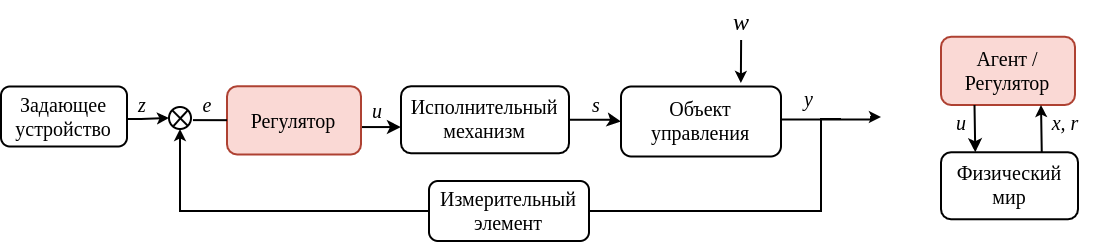
\includegraphics[width=0.8\linewidth]{my_folder/figure/schema/TAY_RL.png}
	\caption{Структурная схема системы управления}
	\label{fig:NA-ch2}
\end{figure}

\textit{Связь адаптивного управления и RL}

Косвенное адаптивное управление, включает блок идентификации, который принимает на вход управляющее воздействие и действительный выход с объекта управления, расчитывает новые параметры, чтобы обновить параметры управления.Данный подход похож на методы RL на основе модели. (\firef{fig:r_adap1-ch2})
%
\begin{figure}[ht!] 
	\centering
	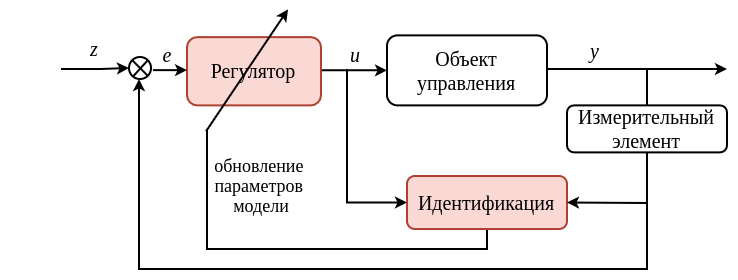
\includegraphics[width=0.8\linewidth]{my_folder/figure/schema/adapt1.png}
	\caption{Косвенное адаптивное управление или модельный RL}
	\label{fig:r_adap1-ch2}
\end{figure}
%

В этом случае идентификация представлена предсказывающим блоком и блоком оценки (\firef{fig:r_adap2-ch2}). На вход блока оценки поступает предсказанный сигнал и действительный сигнал, в случае, если различие между сигналами превосходит некоторого заданного порога, критик инициирует обновление параметров блока предсказателя. Данный подход аналогичен имитационному обучению, где цель RL формируется не на основе функции награды, а на основе экспертных около-оптимальных данных.
\begin{figure}[ht!] 
	\centering
	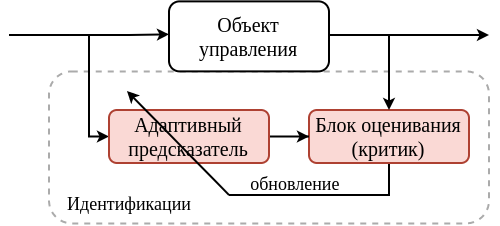
\includegraphics[width=0.4\linewidth]{my_folder/figure/schema/adapt2.png}
	\caption{Идентификация или имитационное обучение}
	\label{fig:r_adap2-ch2}
\end{figure}
%
В прямом адаптивном управлении явно не задается модель системы (\firef{fig:r_adap-ch2}), а используется специальный механизм для сравнения желаемого значения сигнала на выходе и действительно, при этом
Прямое адаптивное управление соответсвует безмодельному RL.
%
\begin{figure}[ht!] 
	\centering
	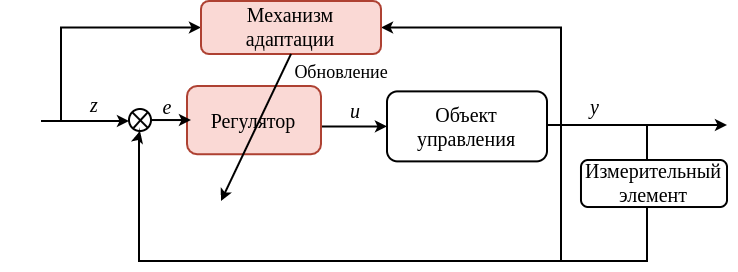
\includegraphics[width=0.4\linewidth]{my_folder/figure/schema/adapt3.png}
	\caption{Прямое адаптивное управление}
	\label{fig:r_adap-ch2}
\end{figure}
Рассмотрим один из основополагающих алгоритмов в RL -- итеративное обучение (\firef{fig:r_adap4-ch2}). Представим этот метод, используя две одинаковые замкнутые системы. Моделирование выполняется на разных итерациях. Первая система запускается на перой итерации, накапливая последовательность рассогласования, генерирует сигнал ошибки, подает его на вход регулятора, который генерирует поправку, на основе минимизации наблюдаемой ошибки. Поправка суммируется с управляющим сигналом регулятора второй система на другом шаге итерации. Такой процесс может выполнятся на каждой итерации с целью подавления помех в замкнутом контуре и минимизации ошибки управления.

\begin{figure}[ht!] 
	\centering
	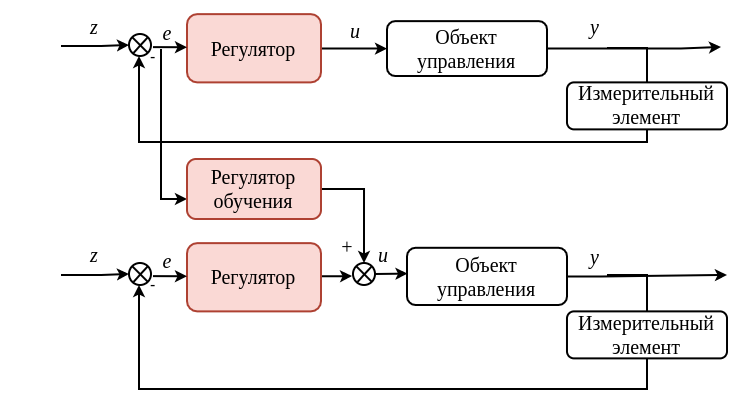
\includegraphics[width=0.6\linewidth]{my_folder/figure/schema/adapt4.png}
	\caption{Итеративное обучение}
	\label{fig:r_adap4-ch2}
\end{figure}


\section{Открытые задачи обучения с подкреплением}

Обучение с подкреплением доказало свою ценность в ряде ограниченных задач, но большую часть исследований в области RL часто трудно использовать в реальных системах из-за ряда допущений, которые редко выполняются на практике \cite{dulac2019challenges}. Ниже перечислены основные нерешенные задачи в области RL, которые необходимо решить, чтобы активно использовать методы RL для управления технических систем:
\begin{itemize}
\item Настройка регулятора на реальной системе на ограниченных образцах.
\item Многомерные непрерывные пространства состояний и действий.
\item Ограничения безопасности, которые никогда или, для определенных объектов, редко должны нарушаться.
\item Частично наблюдаемые системы, альтернативно рассматриваются как нестационарные или стохастические.
\item Сложность формализации функционала качества (функции награды), в частности, для многоагентных систем.
\item Интерпретируемость результатов синтеза регуляторов на базе RL.
\item Расчет управляющее воздействие на частоте работы системы.
\item Большие или неизвестные задержки в исполнительных или измерительных механизмах системы.
\end{itemize}
В отличие от большинства исследований в области RL, в реальных системах нет отдельной среды настройки и оценки. Все данные для обучения поступают из реальной системы, регулятор должен работать достаточно хорошо и действовать безопасно на протяжении всей настройки (обучения). Для многих систем это означает, что исследование должно быть ограничено, в результате поступающие данные будут иметь низкую дисперсию -- небольшая часть пространства состояний может быть исследована. Кроме того, поскольку часто существует только один экземпляр системы, подходы, которые создают экземпляры сотен или тысяч сред для сбора большего количества данных для распределенного обучения, не могут быть применены. В случае, если существуют собранные автономные данные по системе, в большинстве случаев они не содержат необходимое количество и охват, которые необходимы существующим алгоритмам RL. Итерации обучения в реальной системе могут занять много времени, так как есть некоторые системы с большим периодом управления -- от одного часа до нескольких месяцев, а ответный сигнал может составлять порядка месяцев (например, управление гидро- и литосферными процессами, онлайн-реклама, эффективность применения лекарственных препаратов). Даже в случае высокочастотных задач управления алгоритм обучения должен быстро настраиваться на потенциальных ошибках без необходимости повторять их несколько раз, прежде чем исправлять их. Таким образом, для обучения в реальной системе требуется, чтобы алгоритм был эффективным и производительным.

В области обучении с подкреплением выделают отдельное направление связанное с разработкой безопасных алгоритмов RL. Безопасное обучение с подкреплением можно определить как процесс разработки закона управления при максимизации функционала, при обеспечении соблюдение ограничений безопасности во время процессов настройки и эксплуатации. Как правило, выделяют два подхода к безопасному обучению с подкреплением.
Первый основан на модификации критерия оптимальности. Второй основан на модификации процесса обучения путем включения внешних знаний, дополнительных ограничений. Может применяется резервный регулятор, который в случае, если закон управления нарушает ограничения безопасности, взять на себя управление. Это своего рода алгоритмическое резервирование управления (\firef{fig:r_safe_rl-ch2})
\begin{figure}[ht!] 
	\centering
	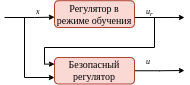
\includegraphics[width=0.4\linewidth]{my_folder/figure/schema/safe_RL.png}
	\caption{один из вариантов}
	\label{fig:r_safe_rl-ch2}
\end{figure}

Есть ряд успешных работ, которые изучают варианты использования функции Ляпунова для доказательства безопасности управления \cite{chow2018lyapunovbased}.

Еще одним важным аспектом реальных систем является то, что они принадлежат и управляются людьми, которые требуют понимания алгоритмов управления. По этой причине интерпретируемость закона управления важна для реальных задач. Особенно в случаях, когда функция имеет альтернативный и неожиданный подход к управлению. В случае ошибок алгоритма управления важно иметь возможность апостериорно понять причину ошибки. Есть ряд работ направленных на исследование данной проблемы, например, с применением предметно-ориентированного языка программирования.

Вывод по главе \thechapter. В ходе анализа и изучения связи между обучением с подкреплением и управлением, сделаны следующие выводы:
\begin{itemize}
	
	\item Обучение с подкреплением -- это параметрический метод аппроксимации функции ценности для решения задачи приближенного динамического программирования;
	\item Обучение с подкреплением, как и приближенное динамическое программирование способно справиться с проблемой проклятья размерности;
	\item Динамическое программирование рассматривается как один из главных способов обучения агента;
	\item Модельное обучение с подкреплением соответствует косвенному адаптивному управлению, безмодельное обучение с подкреплением соответствует прямому адаптивному управлению;
	\item Главные нерешенные задачи обучения с подкреплением -- это описание функции награды и обеспечение безопасности как во время настройки регулятора, так и во время эксплуатации;
\end{itemize}	         	 % Глава 2
\newpage
\chapter{Применение методов обучения с подкреплением в задаче разработки регуляторов для сложных систем управления} \label{ch3}

% не рекомендуется использовать отдельную section <<введение>> после лета 2020 года
%\section{Введение} \label{ch3:intro}

В данной главе будут рассмотрены практические примеры применения алгоритмов RL для задачи управления обратного маятника и сложных систем, которые описываются моделями типа <<хищник-жертва>>: развитие опухоли, производство пенициллина. 
	
\section{Задача управления обратным маятником} \label{ch3:sec1}
Рассмотрим следующую математическую модель перевернутого маятника:
%
\begin{equation*}
%\label{pendulum}
\ddot \vartheta_t = -0.01 \dot \vartheta_t + 9.8 \sin \vartheta_t - U_t \cos \vartheta_t
\end{equation*}
%
где $\vartheta_t \in \mathbb{R}$ -- угол наклона маятника; $U_t \in \mathcal{U}$ -- крутящий момент приложенный к маятнику в момент времени $t$. Параметры модели маятника: \(m\) = 1 кг; \(l\) = 1 м; \(g\) = 9.8 м/с²; \(\mu\) = 0.01;
Пространство действий может быть задано как $\mathcal{U}=[-u_{max},u_{max}] \subset \mathbb{R}$, при ограничении $u_{max} = 5$ Н $\cdot$ м. Динамика системы может быть представлена как:
%
\begin{equation*}
	f_d(x) = 
	\begin{bmatrix}
		x_2 \\
		9.8 \sin x_1 - 0.01x_2
	\end{bmatrix}
	, F_c(x)=
	\begin{bmatrix}
		0\\
		-\cos x_1
	\end{bmatrix}
\end{equation*}
%
где $x = [x_1, x_2]^T \in \mathbb{R}^2$. При моделировании устанавливаем коэффициент дисконтирования равный $\gamma = 0.1$ и шаг по времени \(\Delta t = 10\) мс.

Цель управления -- качнуть вверх и, в конечном итоге, установить маятник в вертикальное положение $2\pi k$ для некоторого $k \in \mathbb{Z}$ при ограничении крутящего момента $|U_t| \leq u_{max}$. 

Нахождение оценки политики $V_i$ на каждой итерации $i$ производится аппроксимируя линейную функцию:
%
\begin{equation*}
V_i(x) \approx V(x; \theta_i) = \theta^T_i \phi(x),
\end{equation*}
где $\theta_i \in \mathbb{R}^L$ - веса и $\phi(x)$ признаки с $L=121$ 

Поскольку для шага улучшения политики требуется дифференцируемая функция, выбрана радиально-базисные функция в качестве признаков $\phi(x)$, следовательно, $j$-я компонента вектора признаков $\phi(x)$ задается как:
%
\begin{equation*}
	\phi_j(x) = \exp(-(x - c_j)^T \Sigma^{-1}(x-c_j))
\end{equation*}
%
где $\Sigma^{-1}$ -- весовая матрица, а $c_j$ - центральные точки радиально базисных функций.

Рассматривается функция вознаграждения $r$, заданная формулами:
\begin{equation*}
r(x,u) = \mathfrak r(x) - \mathfrak c(u)
\end{equation*}
где $\mathfrak r(x)$ и $\mathfrak c(u)$ для непрерывного управления, применяя алгоритм DPI, имеют следующий вид:
	\begin{equation*}
	\begin{split}
	\mathfrak r(x) &= \cos x_1\\
	\mathfrak c(u) &= \lim_{v->u} \int_0^v {(s^T)^{-1}}(\mathfrak u) \cdot \text{Г} du\\
	s(\mathfrak u) &= u_{\max} \tanh(\mathfrak u/u_{\max})\\
	\end{split}
	\end{equation*}

При этом функция $s$ задает ограничения модели. Г - положительно определенная матрица.
%
Для решения задачи управления, был использован следующий метод обучения с подкреплением: \textit{Дифференциальная оценка по стратегиям} (англ. Differential Policy Iteration, DPI) ~---
алгоритм оценивает и улучшает стратегию, начиная от начальной допустимой стратегии \( \pi_0 \) и до тех пор, пока оценка и стратегия не сойдутся. На этапе оценки стратегии производится расчет дифференциального уравнения Беллмана, чтобы получить функцию стоимости \(v_i = v_{\pi_{i-1}}\) для последней стратегии \( \pi_{i - 1} \):
\begin{equation}
\alpha \cdot v_i(x) = h(x, \pi_{i-1}(x), \nabla v_i(x))   \forall x \in X
\end{equation}
Далее рассчитанное значение \(v_i\) используется в улучшении стратегии, то есть для получения следующей стратегии \( \pi_i \)  путем минимизации гамильтониана:
\begin{equation}
\pi_i(x) \in \arg \underset{u \in U}{\min}  h(x,u, \nabla v_i(x))   \forall x \in X
\end{equation}

Стоит отметить, что при использовании алгоритма дифференциальной оценки по стратегиям необходимо иметь формализованную модель ОУ (на первом шаге алгоритма рассчитывается гамильтониан). В работе \cite{DBLP:journals/corr/LeeS17a} представлен схожий алгоритм, который позволяет отказаться от использования модели объекта, который в рамках данной работы рассмотрен не был. Но в дальнейшем представляет особый интерес, так как данные методы направлены на работу в непрерывном времени и пространстве.
Результат работы регулятора для перевернутого маятника при ограничениях представлен на \firef{fig:pend-ch3}.
%
\begin{figure}[ht!]  
	\centering 
	\begin{minipage}[h]{0.49\linewidth}
		\center{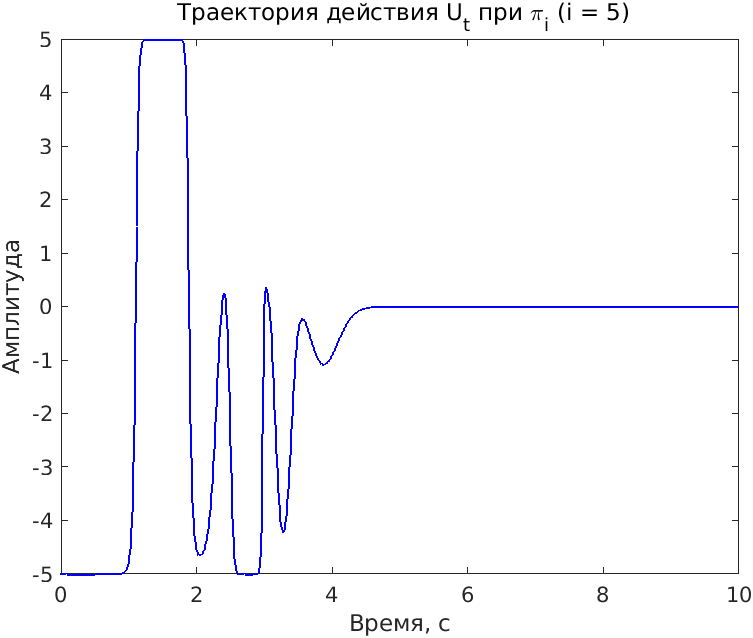
\includegraphics[width=0.9\linewidth]{my_folder/figure/pendul/action.png}\\ \textit{a}}
	\end{minipage}
	\hfill
	\begin{minipage}[h]{0.49\linewidth}
		\center{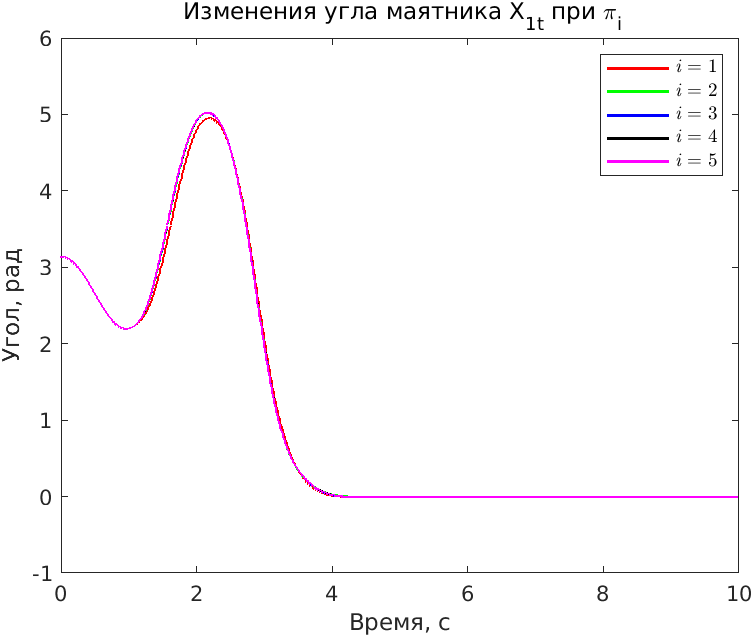
\includegraphics[width=0.9\linewidth]{my_folder/figure/pendul/traj_.png}\\ \textit{б}}
	\end{minipage}
	\hfill
	\begin{minipage}[h]{0.49\linewidth}
		\center{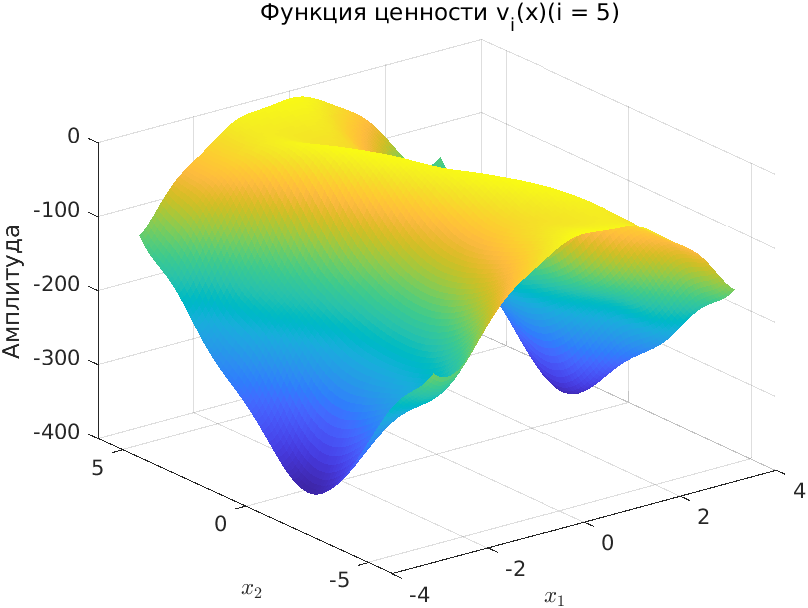
\includegraphics[width=0.9\linewidth]{my_folder/figure/pendul/val_fun.png}\\ \textit{в}}
	\end{minipage}
	\hfill
	\begin{minipage}[h]{0.49\linewidth}
		\center{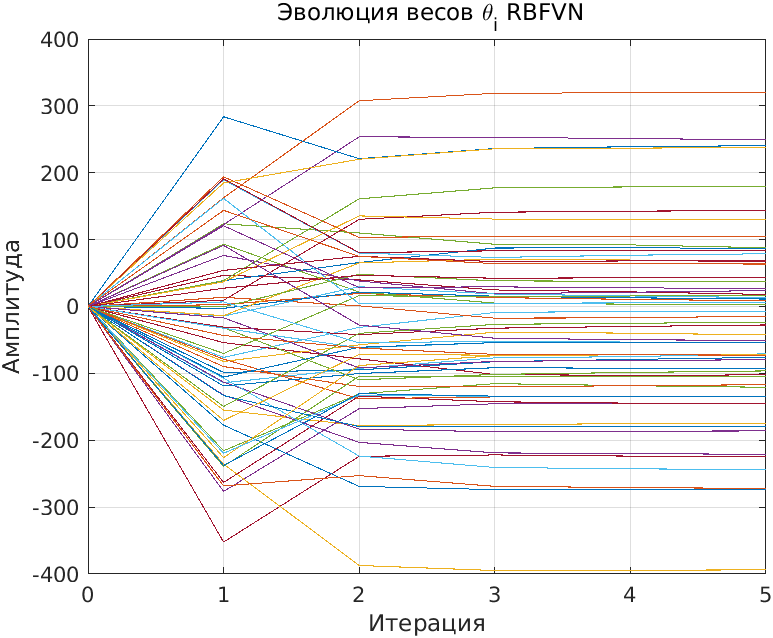
\includegraphics[width=0.85\linewidth]{my_folder/figure/pendul/w.png}\\ \textit{г}}
	\end{minipage}
	\caption{Применение алгоритма DPI для задачи управления обратным маятником; \textit{a} -- управляющее воздействие; \textit{б} -- изменение угла наклона маятника; \textit{в} -- изменение функционала качества; \textit{г} -- график изменения весов}
	\label{fig:pend-ch3}
\end{figure}

%
\section{Управление производством пенициллина}\label{ch3:sec2}
%
Модель биореактора описывает поведение двух видов, которые соревнуются за один субстрат. Реализация систем автоматизации для биореакторов ограничена сложностью синтеза регулятора для систем с большим количеством переменных. Так же автоматизация таких систем ограничена сложностью описания внешних воздействий (например учет воздействия кислорода и углекислого газа на систему), поэтому возникает интерес реализации оптимально-адаптивных регуляторов для таких систем.

В качестве примера рассмотрена модель производства пенициллина  периодического действия \cite{bajpai1980mechanistic}.
Модель была основана на следующих предположениях: 1) рост клеток ограничен субстратом (глюкозой) и кислородом, 2) вся биомасса способна расти и синтезировать пенициллин, 3) образование продукта подавляется субстратом, и 4) требования к техническому обслуживанию постоянны \cite{patnaik2001penicillin}. Модель системы описывается системой однородных дифференциальных уравнений:
%
\begin{equation}\label{eq:penicilin}
\begin{split}
\dot{X} &=\mu(S)X-\frac{u_{\text{inp}}}{V}X,\\
\dot{S} &=-\frac{\mu(S)X}{Y_{\text{x}}}-\frac{vX}{Y_{\text{p}}}+\frac{u_{\text{inp}}}{V}(S_{\text{in}}-S),\\
\dot{P} &=vX-\frac{u_{\text{inp}}}{V}P,\\
\dot{V} &=u_{\text{inp}},\\
\end{split}
\end{equation}
где удельная скорость роста продукта:
\begin{align*}
	\mu(S)&=\frac{\mu_m S}{K_{\text{m}}+S+(S^2/K_{\text{i}})},
\end{align*}
где $X$ -- концентрация биомассы (г/л), $S$ -- концентрация субстрата (г/л), $P$ -- концентрация продукта (г/л), $V$ -- объем биомассы в биореакторе. Управляющим входом является $u$ -- скорость подачи субстрата (г/(л ч)). Параметры модели представлены в \taref{table:penicilin-ch3}
%
\begin{table}[h!]
	\centering
	\small
	\caption{Параметры модели производства пенициллина}
	\begin{tabular}{|p{50pt}|p{190pt}|p{50pt}|p{110pt}|}
		\hline
		
		Параметр  & Описание параметра  & Величина  & Единица измерения  \\
		\hline
		$S_{in}$ & концентрация субстрата в корме & 0.2 & л / (г/л)\\
		\hline
		$Y_x$ & доходность биомассы на единицу массы субстрата & 0.2 & л / (г / ммоль O2)\\
		\hline
		$Y_p$ & доходность продукта на единицу массы субстрата & 1.2 & л /((г / ммоль O2)\\
		\hline
		$\mu_m$& максимальная удельная скорость продукта d &0.02& 1/ч\\
		\hline
		$v$& удельная скорость роста биомассы & 0.004 & 1/ч\\
		\hline
		$K_m$ & константа Моно  & 0.05 & г/л \\
		\hline
		$K_i$ & константа ингибирования  & 5.0 & г/л \\
		\hline
	\end{tabular}
	\label{table:penicilin-ch3}
\end{table}

Цель управления -- получение максимальной концентрации продукта $P$. Задача оптимального управления может быть сформулирована следующим образом:
%
\begin{equation}
\label{f:optimal_task}
\begin{split}
J &= \min_{u, t_f}(\int^{t_f}_0 P(\tau) d\tau) \\
\mathbf{x} &= [X\ S\ P \ V], \space \mathbf{x}(0) = [1.0 \ 0.5 \ 0.01 \ 120.0]^T\\
\dot{\mathbf{x}} &= f(\mathbf{x},u) \\
0 &\le u \le 0.2,\ \  0 \le X\le 3.7, \ \ 0 \le P\le 3.0 \\
0 &\le V \le 125,\ \ S \ge 0 \\
\end{split}
\end{equation}

Для данного объекта управления было реализовано три типа регулятора: оптимальный регулятор, полученный численными методами, регулятор онлайн-оптимизации MPC и регулятор на основе обучения с подкреплением -- Глубокие детерминированные градиенты политики (англ. Deep Deterministic Policy Gradient, DDPG). Используя пакетный модуль OpenOCL, реализованный на языке MATLAB найдено численное решение оптимального управления для модели производства пенициллина. При разработке системы управления методом RL функция награды имела следующий вид: $r = lg(P_k/P_{k-1}) - 50*[X>3.7]-50*[P>3.0]-50*[V>125]$. Результаты моделирования представлены на \firef{fig:bio-ch3}
%
\begin{figure}[ht!]  
	\centering 
	\begin{minipage}[h]{0.49\linewidth}
		\center{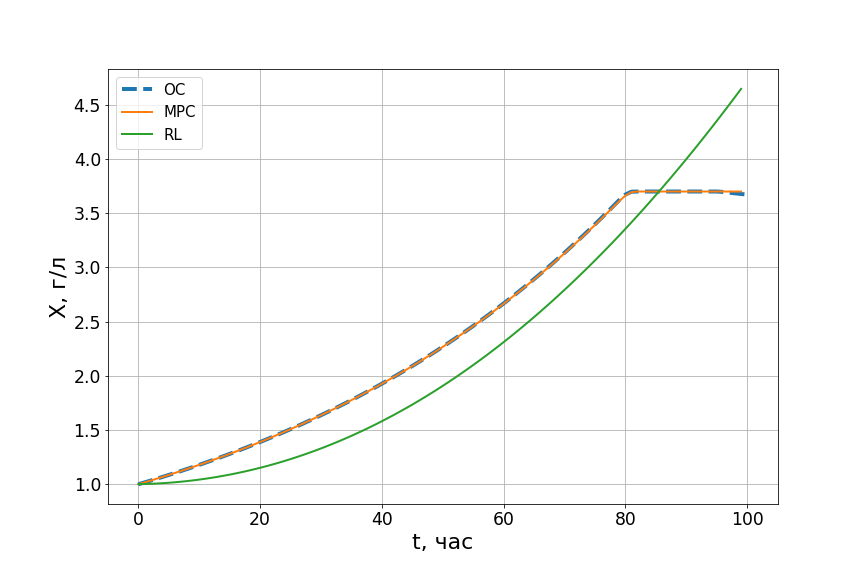
\includegraphics[width=1\linewidth]{my_folder/figure/figure_penicillin/x_MPC_RL.png}\\ \textit{a}}
	\end{minipage}
	\hfill
	\begin{minipage}[h]{0.49\linewidth}
		\center{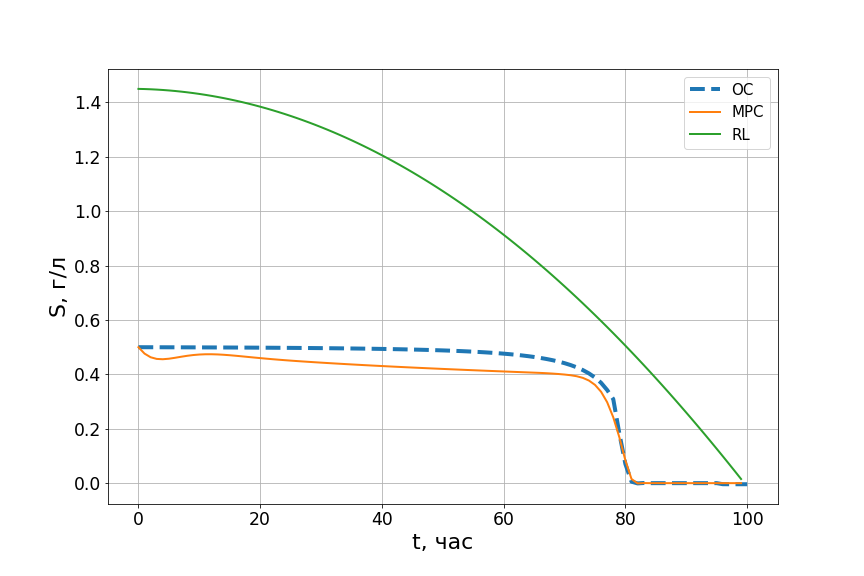
\includegraphics[width=1\linewidth]{my_folder/figure/figure_penicillin/s_MPC_RL.png}\\ \textit{б}}
	\end{minipage}
	\hfill
	\begin{minipage}[h]{0.49\linewidth}
		\center{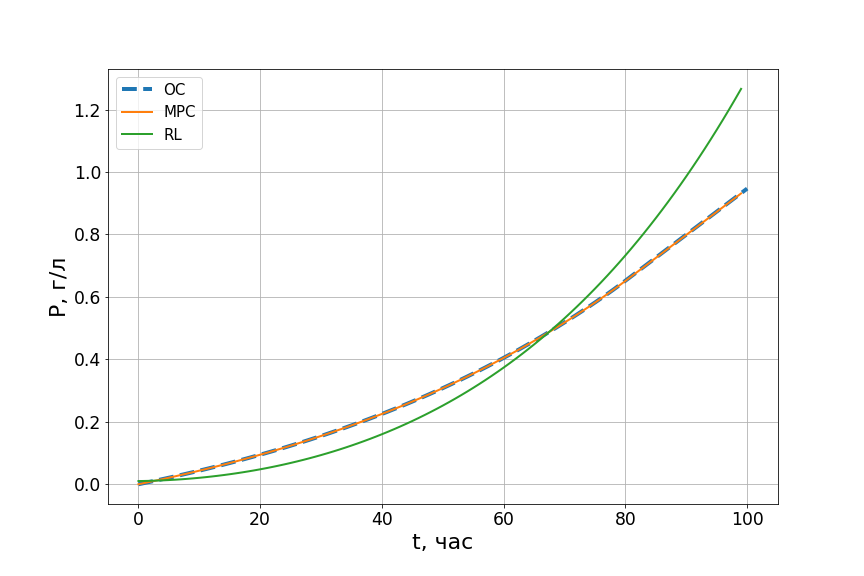
\includegraphics[width=1\linewidth]{my_folder/figure/figure_penicillin/p_MPC_RL.png}\\ \textit{в}}
	\end{minipage}
	\hfill
	\begin{minipage}[h]{0.49\linewidth}
		\center{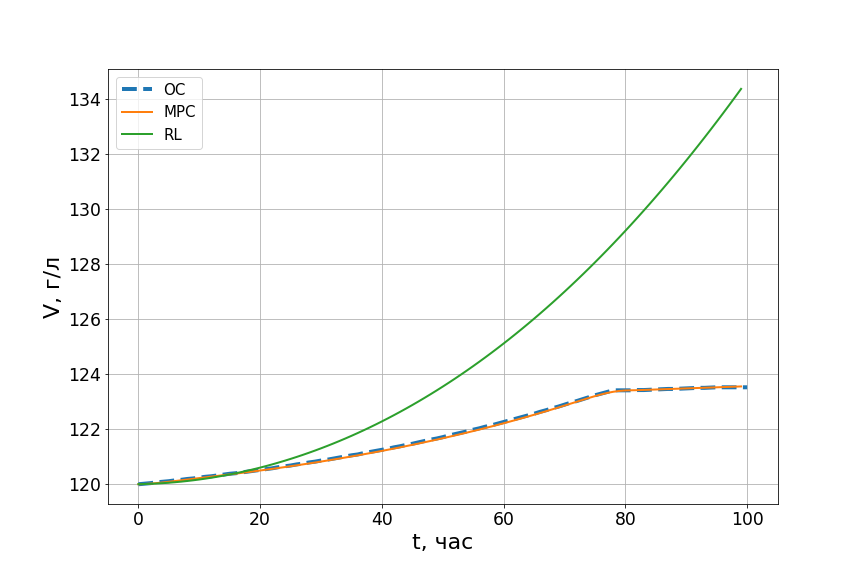
\includegraphics[width=1\linewidth]{my_folder/figure/figure_penicillin/v_MPC_RL.png}\\ \textit{г}}
	\end{minipage}
	\caption{Моделирование управления производства пеницилина: \textit{а} -- изменения концентрации биомассы, \textit{б} -- изменения концентрации субстрата, \textit{в} -- изменения концентрации продукта, \textit{г} -- изменения заполненного объема в биореакторе}
		\label{fig:bio-ch3}
	\end{figure}
%

Для данного процесса важным критерием качества является конечное значение концентрации пенициллина в реакторе $P$. Различие траекторий управляющих воздействий \firef{fig:u_penicillin-ch3} обосновывается не удовлетворительным выбором функции награды, которое предполагается составлять вместе с экспертом. 
\begin{figure}[ht!]
	\center{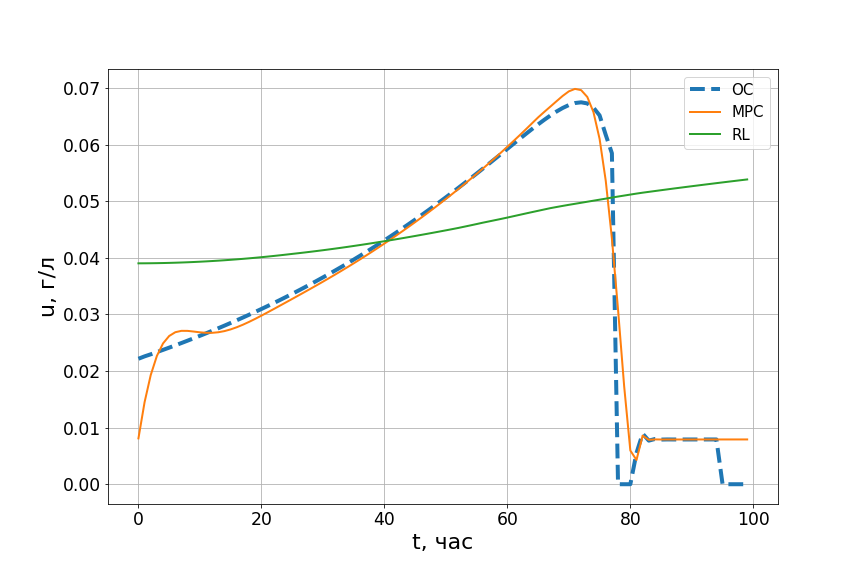
\includegraphics[width=0.5\linewidth]{my_folder/figure/figure_penicillin/u_MPC_RL.png}}
	\caption{Управляющее воздействие, а именно скорость подачи субстрата в реактор}
	\label{fig:u_penicillin-ch3}
\end{figure}


\section{Управление ростом опухоли}\label{ch3:sec2}
%
Рак -- это общее название группы заболеваний, которые включают повторяющееся и неконтролируемое деление и распространение аномальных клеток. Эти аномальные ткани называются опухолями. Ранняя диагностика и эффективное лечение повышают выживаемость больных. Оптимальный график лечения и доза лекарства варьируются в зависимости от стадии опухоли, веса пациента, уровней лейкоцитов (иммунных клеток), сопутствующего заболевания и возраста пациента. Таким образом, правильное планирование и персонализация химиотерапевтического лечения жизненно важны для снижения уровня смертности. 
Чтобы вычислить оптимальную политику управления и вознаграждение, требуется математическая модель, которая показывает воздействие химиотерапевтического препарата в динамике. Реалистичная модель должна учитывать рост опухоли, реакцию иммунной системы человека на рост опухоли и влияние химиотерапевтического лечения на иммунные клетки, нормальные клетки и рост опухоли.

Одна из основных проблем, связанных с изучением рака как динамической системы, состоит в том, что как и любое другое заболевание, известен своей сложной, нелинейной и неопределенной механикой действия. Следовательно, математические модели в дифференциальных уравнениях не в состоянии учесть все вариации в динамике пациента, поэтому поставлена задача разработки регулятора на основе обучения с подкреплением.

В работе \cite{kuznetsov1994nonlinear} представлена фармакологическая модель химиотерапии рака, заданная нелинейной системой из 4-х детерминированных однородных дифференциальных уравнений:
\begin{equation}
\begin{split}
\dot T &= r_1T(1-b_1T) - c_2IT-c_3TN-a_2(1-e^{-M})T,\\
\dot N &= r_2N(1-b_2N) - c_4TN-a_3(1-e^{-M})N, \\
\dot I &= s + \frac{\rho IT}{\alpha + T} - c_1IT - d_1I - a_1(1-e^{-M})I, \\
\dot M &= u(t) - d_2M
\end{split}
\end{equation}
где $T(t)$ -- концентрация раковых клеток,  $N(t)$ -- концентрация нормальных клеток $I(t)$ -- концентрация иммунных клеток в крови (лейкоцитов), и $M(t)$ -- концентрация химиотерапевтического препарата в крови. Управляющее воздействие $u(t)$ соответствует скорости ввода препарата (мг/(л день)). Параметры модели представлены в \taref{table:plana-ch3}.
%
\begin{table}[h!]
	\centering
	\small
	\caption{Параметры модели опухоли}
	\begin{tabular}{|p{45pt}|p{210pt}|p{50pt}|p{100pt}|}
		\hline
		Параметр  & Описание параметра  & Величина  & Единица измерения  \\
		\hline
		$a_1$ & скорость фракционного уничтожения иммунных клеток & 0.2 & л / (мг день)\\
		\hline
		$a_2$ & скорость фракционного уничтожения опухолевых клеток & 0.3 & л / (мг день)\\
		\hline
		$a_3$ & скорость фракционного уничтожения нормальных клеток & 0.1 & л / (мг день)\\
		\hline
		$b_1$ & взаимная несущая способность опухолевых клеток & 1 & 1 / клетка\\
		\hline
		$b_2$ & взаимная несущая способность нормальных клеток & 1 & 1 / клетка\\
		\hline
		$c_1$ & срок конкуренции иммунных клеток (конкуренция между опухолевыми и иммунными клетками) & 1 & 1 / (клетка день)\\
		\hline
		$c_2$ & срок конкуренции опухолевых клеток (конкуренция между опухолевыми и иммунными)& 0.5 & 1 / (клетка день)\\
		\hline
		$c_3$ & срок конкуренции опухолевых клеток (конкуренция между нормальными и опухолевыми) & 1 & 1 / (клетка день)\\
		\hline
		$c_4$ & срок конкуренции нормальных клеток конкуренция между нормальными и опухолевыми) & 1 & 1 / (клетка день)\\
		\hline
		$d_1$ & Темп гибели иммунных клеток & 0.2 & 1 / день\\
		\hline
		$d_2$ & Скорость распада вводимого медицинского препарата & 1 & 1 / день\\
		\hline
		$r_1$ & Скорости роста опухолевых клеток (на единицу) & 1.5 & 1 / день\\
		\hline
		$r_2$ & Скорости роста нормальных клеток (на единицу) & 1 & 1 / день\\
		\hline
		$s$ & Скорость притока иммунных клеток & 0.33 & клетка / день\\
		\hline
		$\alpha$ & Скорость иммунного порога (порогового входа) & 0.3 & клетка \\
		\hline
		$\rho$ & Скорость иммунного ответа & 0.01 & 1 / день\\
		\hline
		
	\end{tabular}
	\label{table:plana-ch3}
\end{table}
%

При разработке схемы лечения важно оптимизировать количество используемого лекарства, чтобы регулировать побочные эффекты химиотерапии, поскольку часто иммунная система пациента ослабевает и становится склонной к опасным для жизни инфекциям, что снижает ее способность искоренить рак. В литературе рассматривается два случая: основной и подготовительный -- несколько нереалистичный случай, в котором цель состоит в том, чтобы искоренить рак независимо от состояния популяции остальных клеток. В обоих случаях начальное условие было одинаковым: [0,7 1 1 0] T.

Задача оптимального управления для упрощенного случая, может быть сформулирована следующим образом:
%
\begin{equation*}
\label{f:optimal_task}
\begin{split}
J &= \min_{u, t_f}(\int^{t_f}_0 T(\tau) d\tau) \\
\mathbf{x} &= [T\ N\ I \ M], \ \ \mathbf{x}(0) = [0.7 \ 1 \ 1 \ 0]^T\\
\dot{\mathbf{x}} &= f(\mathbf{x},u) \\
0 &\le u \le 10 
\end{split}
\end{equation*}

Тогда как такую задачу в терминах RL, опираясь на гипотезу о награде сформировать в виде функции вознаграждения: $R = -dt \cdot T$. В этом случае dt включено в вознаграждение только для того, чтобы упростить сравнение с функционалом качества, приведенного в постановке задачи оптимального управления.
Решением такого случае станет подача максимального значения управляющего воздействия на вход системы. 

Рассмотрим реальный случай. Чтобы гарантировать безопасность пациента во время лечения, к постановке (\ref{f:optimal_task}) добавлены дополнительные ограничения состояния. В частности $N (t) \ge 0,4$ и $I (t) \ge 0,4$
Для задачи RL награда будет равна:
\begin{equation*}
	R = dt \cdot (-T - 0.5 \cdot [N < 0.4] - 0.5 \cdot [I < 0.4])
\end{equation*}


На рисунке приведены графики моделирования при оптимальном управления, регулирования на основе MPC и регулятора на основе алгоритма обучения с подкреплением расширения глубоких детерминированных градиентов политики (англ. Twin Delayed Deep Deterministic Policy Gradients, TD3). Результаты моделирования при регулировании представленны на \firef{fig:tumor-ch3} и \firef{fig:u-ch3}.

\begin{figure}[ht!]  
	\centering 
	\begin{minipage}[h]{0.49\linewidth}
		\center{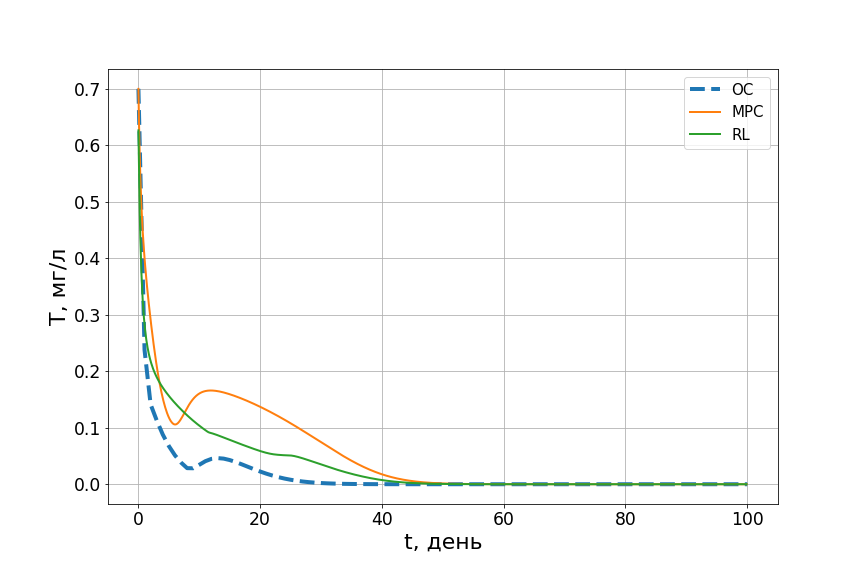
\includegraphics[width=1\linewidth]{my_folder/figure/tumor/T_MPC_RL.png}\\ \textit{a}}
	\end{minipage}
	\hfill
	\begin{minipage}[h]{0.49\linewidth}
		\center{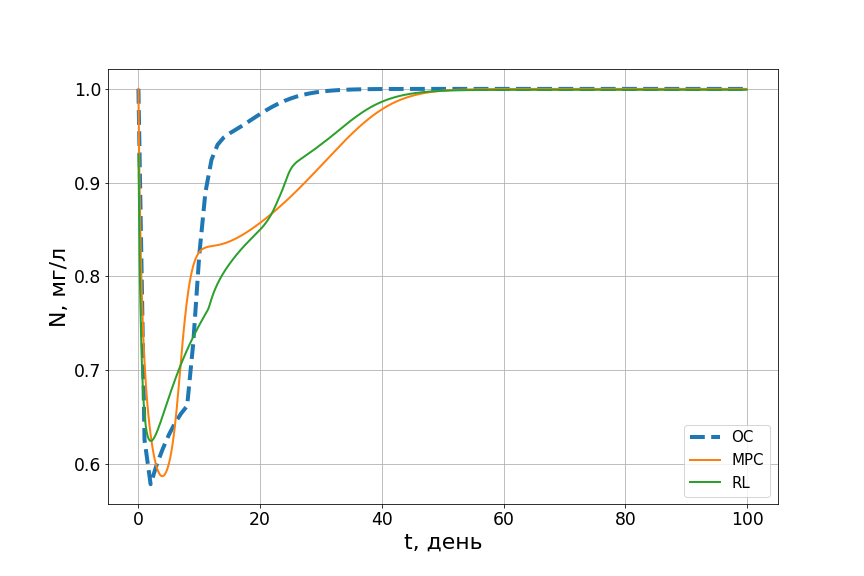
\includegraphics[width=1\linewidth]{my_folder/figure/tumor/N_MPC_RL.png}\\ \textit{б}}
	\end{minipage}
	\hfill
	\begin{minipage}[h]{0.49\linewidth}
		\center{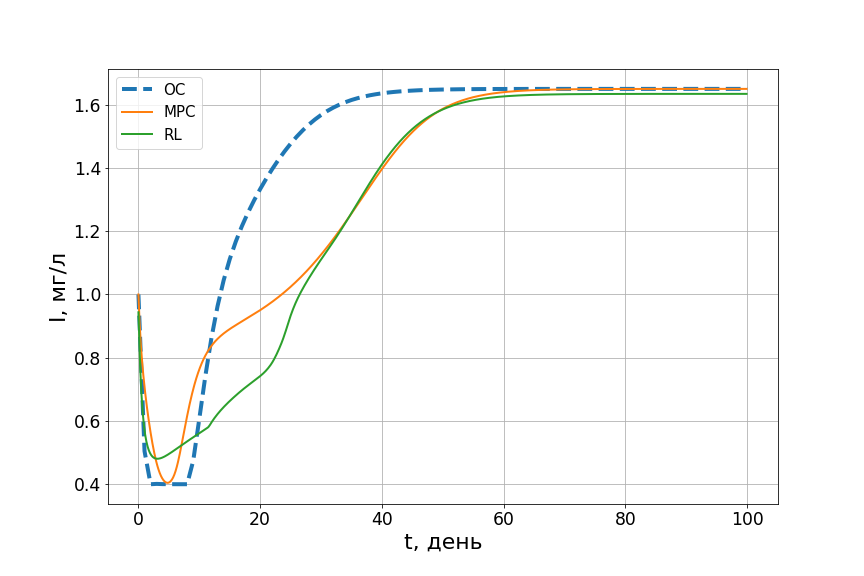
\includegraphics[width=1\linewidth]{my_folder/figure/tumor/I_MPC_RL.png}\\ \textit{в}}
	\end{minipage}
	\hfill
	\begin{minipage}[h]{0.49\linewidth}
		\center{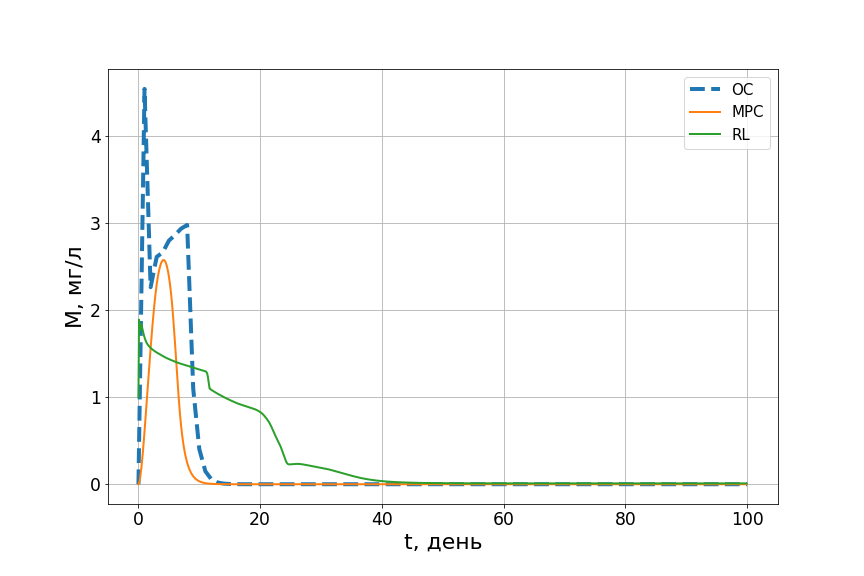
\includegraphics[width=1\linewidth]{my_folder/figure/tumor/M_MPC_RL.png}\\ \textit{г}}
	\end{minipage}
	\caption{Моделирование управления ростом опухоли: \textit{а} -- изменение концентрации раковых клеток, \textit{б} -- изменение концентрации нормальных клеток, \textit{в} -- изменение концентрации иммунных клеток в крови (лейкоцитов), \textit{в} изменение концентрации химиотерапевтического препарата в крови}
	\label{fig:tumor-ch3}
\end{figure}
\begin{figure}[ht!]
	\center{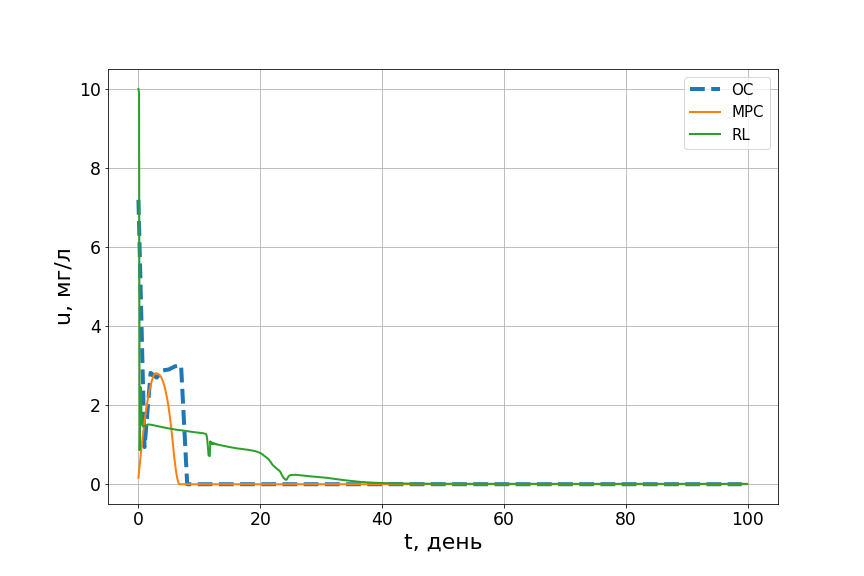
\includegraphics[width=0.65\linewidth]{my_folder/figure/tumor/u_MPC_RL.png}}
	\caption{Управляющее воздействие, представленное скоростью ввода препарата }
	\label{fig:u-ch3}
\end{figure}


Вывод по главе \thechapter. В ходе проведения модельных экспериментов и разработки регуляторов для сложных объектов было установлено:
\begin{itemize}
	
	\item Эксперимент по разработке регулятора для управления производством пенициллина показал, что качество работы безмодельных алгоритмов обучения с подкреплением сильно зависит от дизайна  функционала качества, что только подтверждает указанную проблему в главе 2;
	\item Для задачи управления перевернутым маятников регулятор на основе модельного алгоритма обучения с подкреплением учел ограничения, которые были указаны при разработке функционала качества; 
	\item Регулятор на основе обучения с подкрепления для задачи управления роста опухоли показал такие же высокие качества управления как оптимальный регулятор и регулятор на основе онлайн оптимизации MPC;
	\item Проведенные эксперименты подтверждают применимость методов обучения с подкреплением для задач управления сложными объектами;
\end{itemize}

\newpage
%% Вспомогательные команды - Additional commands
%
%\newpage % принудительное начало с новой страницы, использовать только в конце раздела
%\clearpage % осуществляется пакетом <<placeins>> в пределах секций
%\newpage\leavevmode\thispagestyle{empty}\newpage % 100 % начало новой страницы           	 % Глава 3
% !TeX spellcheck = russian_english
\chapter{Разработка бизнес-плана по коммерциализации проекта} \label{ch4}
\section{Описание проекта}

\textit{Резюме.} Бизнес-план посвящен оценки рентабельности оказания услуги по разработке алгоритмов управления сложных технических систем с применением методов обучения с подкреплением.
Потенциальные заказчики услуги -- промышленные предприятия и компании в области разработки и проектирования автоматизированных систем управления технологическим процессом (АСУ ТП). Для существующих подходов в управлении отдельными техническими системами на рынке АСУ ТП характерна высокая стоимость и длительный цикл разработки. Поэтому предлагается использовать методы обучения с подкреплением, с целью уменьшить время разработки, без потери качеств управления.

В первый квартал планируется реализация и внедрение двух алгоритмов автоматизации, стоимость каждого -- 700 000 рублей. В последующие кварталы планируется объем -- 3 единиц услуг, по 500 000 рублей каждая.
В связи со спецификой технологии оказываемых услуг, необходимо проводить активную кампанию по продвижению услуги на рынке, что подразумевает затраты на рекламу в размере 90 600 рублей без НДС в первый год оказания услуг.
Бизнес-план составлен на прогнозный период 1 год. Срок организации бизнеса составляет 1 месяц, предполагается, что со 2-го месяца проект начнет приносить доход. В качестве расчетов принят календарный год с мая по апрель. Для расчета инвестиционной привлекательности проекта использовались следующие допущения:
\begin{itemize}
\item организация использует общую систему налогообложения;
\item налог на добавленную стоимость (НДС) – 20\%;
\item отчисления работодателя с доходов сотрудника – 30\%;
\item налог на прибыль – 20\%.
\end{itemize}

Полученные показатели инвестиционной привлекательности проекта с учетом ставки дисконтирования (20 \%): 
\begin{itemize}
\item сумма инвестиций (I) составляет 500 000 рублей;
\item чистая текущая стоимость проекта (NPV) составляет 1 830 000 рублей;
\itemсрок окупаемости проекта составит 1 квартал.
\end{itemize}
Полученные показатели указывает на экономическую целесообразность осуществления проекта с учетом ограничений и допущений в бизнес-плане.


\textit{Описание продукции}.Описание услуги: Разработка алгоритмов интеллектуальных систем управления сложных технологических объектов с применением методов обучения с подкреплением.

Цифровизация промышленности и, как следствие, автоматизация производственных процессов - современный тренд, движение в сторону которого, обеспечивает предприятиям высокую гибкость в формировании бизнес-моделей и широкий охват потенциальной клиентской базы посредством интеграции киберфизических систем и интернета вещей в производственный процесс. В основе внедрения новых технологий лежит стремление к комплексному повышению эффективности и созданию условий для успешной работы предприятия. Промышленные компании сталкиваются с задачами снижения издержек, сокращения сроков вывода новой продукции на рынок, улучшения эффективности всех процессов, поскольку требования со стороны потребителей данной услуги каждый год растут.
Поэтому, со стороны производства возникает запрос на автоматизацию производственных процессов, с применением современных технологий, которые смогут обеспечить адаптивность, отказоустойчивость и оптимальность процессов. 
Компания Forrester указывает в своем отчете, что 20\% компаний создадут инновационные цифровые подразделения в ближайшие годы. То есть ряд промышленных предприятий будет пробовать реализовывать и внедрять новые технологии автоматизации самостоятельно. Существует ряд компаний, которые уже давно на рынке и готовы внедрять надежные системы автоматизации, с помощью традиционных подходов. 
Компании, которые в настоящее время поставляют системы автоматического управления, при синтезе регуляторов, по большей части, используют классические подходы теории автоматического управления. Тогда как наука шагнула вперед и теперь существуют лучшие подходы в разработке алгоритмов управления технических систем.

Обращаясь к традиционным подходам в управлении сложных технических систем при создании систем автоматического управления необходимо иметь точную математическую модель объекта управления (ОУ). Во многих реальных задачах построение такой модели либо невозможно, либо требует проведения трудоёмких исследований. При этом параметры ОУ могут изменяться в широких пределах в процессе функционирования системы, либо иметь большой разброс значений от образца к образцу. В таких случаях регуляторы с постоянными настройками не всегда могут обеспечить требуемое качество работы системы. 

Если обратиться к области машинного обучения, то существует ряд методов, которые могут помочь в задаче управления технических систем. Обучение с подкреплением -- группа методов, при которых алгоритм учится выполнять задачу, многократно взаимодействуя с симулятором динамической системой. Это происходит без прямого вмешательства человека и без необходимости программировать алгоритм для выполнения конкретной задачи.

В рамках данного проекта предлагается услуга по разработке алгоритмов управления на основе методов обучения с подкреплением и внедрение их в микроконтроллеры. 

Технические характеристики предоставляемой услуги будет:
\begin{enumerate}[1.]
	\item Алгоритм регулирования на высокоуровневом языке программирования;
	\item Подключения к оборудованию по промышленным протоколам передачи данных;
	\item Визуализация работы алгоритма, создание автоматизированных отчетов;
	\item Алгоритм конвертации кода на промышленный язык программирования.
\end{enumerate}

Самая большая проблема рынка автоматизации производства -- это первоначальная стоимость инвестиций, необходимых для проектирования, выполнения и установки автоматизированной системы, а так же малое колличество подготовленных специалистов на стыке разных дисциплин. Предполагается, что предоставляя услугу по разработке алгоритмов управления с использованием обучения с подкреплением, можно в разы ускорить и удешевить процесс разработки регуляторов, увечив качество управления за счет адаптации к системе.
Так же сложности возникают, если на предприятии уже имеется оборудование автоматизации отдельного производителя, предлагаемая услуга не привязана к модели контроллеров, датчиков или исполнительных механизмов. То есть является универсальным решением для АСУ ТП.


\textit{Анализ рынка сбыта.} По данным аналитиков компании Fortune Business Insights, к 2026 году рынок промышленной автоматизации вырастет до суммы в \$310 миллиардов, при совокупном среднегодовом темп роста около 8,5\%.
Оценивая основные экономические характеристики отрасли, отметим, что объем российского рынка АСУ ТП в 2020 году составил 58,7 млрд рублей, подсчитали аналитики компании J’son \& Partners Consulting \cite{eco_1}. Рынок находится на растущем этапе развития, следовательно и сегменту по разработке программного обеспечения присущ рост. На рынке заметна нехватка мощностей, что вызвано стимуляцией цифровизации промышленности со стороны государства. 
Ожидается, что усиленное внимание к повышению производительности и стремление к устранению опасных ручных процессов с привлечением человека -- станет основными движущими силами в ближайшие несколько лет. Отдельно стоит отметить, что пандемия коронавируса уже стала одним из факторов роста рынка автоматизации.

На рынке АСУ ТП можно выделить минимум 2 сегмента по цене. Так как сложно найти информацию по средней цене, затрачиваемой предприятиями на автоматизацию, стоит отметить, что рассматриваемая услуга будет направлена на предприятия среднего и ниже среднего ценового сегмента. Например, такие компании как ПАО «СИБУР Холдинг», ПАО «Газпром» могут позволить себе полноценный комплекс автоматизации от ключевых игроков рынка (Siemens, Schneider Electric и т.д.), которые помимо классических решений регулирования, так же предлагают современные адаптивно-оптимальные подходы. Но в данном случае существует привязка к оборудованию. Данных проект направлен на заказчиков, которые имеют оборудования автоматизации от разных производителей и при этом доход таких компаний относится к средним показателям по рынку автоматизации.

Потенциальные заказчики услуги:
\begin{itemize}
\item Промышленные предприятия среднего ценового сегмента;
\item Компании в области разработки и проектирования АСУ ТП среднего ценового сегмента.
\end{itemize}

Высокие затраты на установку и техническое обслуживание, а также отсутствие квалифицированных специалистов являются одними из ограничений в этой отрасли.
Услуга охватывает все сегменты предприятий по отраслям: нефтегазовая, металлургическая и горнодобывающая, фармацевтическая, целлюлозно-бумажная, автомобильная, химическая и т.д. Для любых производственных компаний, занимающихся данной деятельностью, важнейшим фактором выживаемости в конкурентной борьбе является постоянное обновление проектов в соответствии с современными стандартами и технологиями.

Лидеры рынка АСУ ТП неизменны на протяжении многих лет, их решения проверены временем и используются на многих предприятиях. Стабильность позиций во многом связана с тем, что производители предлагают законченную инфраструктуру, и с точки зрения эксплуатации клиентам выгодно иметь оборудование одного вендора, так как это облегчает поиск и замену оборудования и комплектующих, а также подготовку обслуживающего персонала.
Ключевыми игроками на рынке автоматизации являются ABB, General Electric, Honeywell Solutions, Emerson Electric, Siemens AG, Schneider Electric, Mitsubishi Electric Corporation,  Rockwell Automation и Yokogawa Electric.

Предложений о разработки алгоритмов с помощью методов обучения с подкреплением в свободных источниках лидирующих компаний в автоматизации нет. Но, предполагается, что лидеры области предлагают такие услуги для предприятий высокого ценового сегмента, и стоимость данной услуги -- велика. Помимо этого ключевые игроки готовы работать с оборудованием автоматизации только собственной поставки, что не всегда удобно для компаний низкого и среднего ценового сегмента.


По охватываемым областям промышленности рынок систем автоматизации подразделяется на следующие сегменты: аэрокосмический и оборонный, автомобильный, химический, энергетический, продуктовый, здравоохранение, металлургия, нефтегазовый.

В промышленном производстве обучение с подкреплением предлагается использовать в процессах, где требуются сложные навыки принятия решений и регулирования, особенно, когда необходимо справляться с изменениями в динамической среде. Например, в процессе эксплуатации параметры оборудования могут изменятся. Другой пример применения алгоритмов обучения с подкреплением -- это разработка алгоритмов управления, используя цифровые двойники. Исследователями из лаборатории промышленного искусственного интеллекта Hitachi America разработали виртуальный цех как двумерную матрицу и использовали алгоритмы обучения с подкреплением для многократного взаимодействия с этой виртуальной средой. По результатам моделирования, исследователи смогли определить лучшую настройку для повышения производительности работы цеха и сокращения задержек поставок.


%Потребность в операционной эффективности, быстрорастущий интерес к Интернету вещей (IoT) и облачной автоматизации, растущий спрос на умные фабрики, групповая настройка агрегатов, синхронизация цепочки поставок, рост НИОКР, инновации в области искусственного интеллекта и развитие коммуникационных технологий M2M являются одними из ключевых факторов интереса к нетрадиционных алгоритмам управления систем. 


\textit{Анализ конкурентов.} Прямых аналогов в выделенном сегменте рынка нет. Потенциальными конкурентами выступают научные лабораторий автоматизации при университетах. Например, лаборатория систем автоматизированного проектирования (САПР) в Санкт-Петербургском Политехническом Университете Петра Великого. Основным преимуществом которой, является наличие учебных стендов, которые могут понадобиться на этапе тестирования алгоритмов. Но данная лаборатория не специализируется в современных методах машинного обучения, поэтому предполагается, что угроза появления конкурента низкая. Проведен конкурентный анализ по модели Партера. Результаты представлены в таблице \ref{tab:part}.
\begin{table}[h!]
	\centering
	\caption{Конкурентный анализ по модели Партера}
	\begin{tabular}{|p{8cm}|p{8cm}|}
		\hline
		Критерий & Вывод \\
		\hline
		Оценка конкурентоспособность товара компании и уровня конкуренции на рынке &  средний уровень угрозы со стороны товаров-заменителей \\
		\hline
		Оценка уровня внутриотраслевой конкуренции & Низкий уровень внутриотраслевой конкуренции \\
		\hline 
		Оценка угрозы входа новых игроков & Высокий уровень угрозы входа новых игроков \\
		\hline
		Оценка  угрозы ухода потребителей  (рыночная власть покупателя) & Низкий уровень угрозы ухода клиентов \\
		\hline
		Оценка угрозы для Вашего бизнеса со стороны поставщиков & Низкий уровень влияния поставщиков \\
		\hline
		
	\end{tabular}
	\label{tab:part}
\end{table}

Будут применены следующие стратегии повышении конкурентноспособности:
дифференциация продукта -- уникальность продукта и его высокое качество и особый подход, своевременное реагирование на потребности рынка -- опережение конкурентов во времени за счет универсальности системы реализации алгоритмов управления. 

\section{План маркетинга}
План маркетинга включает в себя план продаж, товарную политику, ценовую политику и сбытовую политику и рекламные мероприятия.

\textit{План продаж.} С учетом роста рынка, на основе метода экспертных оценок сформирован прогнозный план продаж табл.~\ref{table:plan_proda}. Ожидаемый объем продаж и цена услуги установлена исходя из высокого спроса и оценки эксперта в области автоматизации.
\begin{table}[h!]
	\centering
	\caption{План продаж}
	\begin{tabular}{|c|c|c|c|c|c|}
		\hline
		\multirow{2}*{Показатели}&\multicolumn{4}{|c|}{Квартал}   & \multirow{2}*{Всего}\\
		\cline{2-5}
		& I & II & III & IV & \\ 
		\hline
		\multicolumn{6}{|c|}{\textit{Разработка алгоритма управления}} \\
		\hline
		Ожидаемы объем продаж, ед.  & 2  & 3  & 3  & 3  & 10  \\
		\hline
		Цена с НДС, т.р.  & 700  & 500  & 500 & 500  & - \\
		\hline
		Выручка с НДС, т.р.   & 1 400  & 1 500  & 1 500  & 1 500  & 5 900 \\
		\hline
		Нетто-выручка (без НДС), т.р.  & 1 120  & 1 200  & 1 200  & 1 200  & 4 720 \\
		\hline
		Сумма НДС, т.р   & 280 & 300 & 300  & 300  & 1 180 \\
		\hline
	\end{tabular}
	\label{table:plan_proda}
\end{table}


\textit{Товарная политика.} Предлагаемый комплекс продуктов: программный код на высокоуровневом языке, техническая документация, алгоритм конвертации модели на язык программирования промышленных контроллеров (стандарта МЭК (IEC 61131-3)), а так же система визуализации качества регулирования. Так же удовлетворены условия качества продукта -- продукт полностью соответствует современным стандартам программного обеспечения, имеет сертифицированный уровень защиты информации.
Дизайн и товарный знак продукта будут уточнены в процессе разработки.
Предполагаемое техническое обслуживание включено в стоимость -- обращение в техническую поддержку за консультациями по работе системы, помощь с первоначальной установкой на программируемый логический контроллер (ПЛК), демонстрация режимов.
Гарантийное обслуживание: компания не несет ответственности за проблемы в работе системы, вызванные аппаратными сбоями, но помощь по восстановлению работы системы после аппаратных сбоев включена в стоимость.

\textit{Ценовая политика.} Метод ценообразования: постоянная базовая составляющая. Цена продукции получена с учетом экспертной оценки: 500 000 р + 100 000 р, в случае дополнительных ограничений. В первый квартал добавленная надбавка по рекомендации специалиста, с целью обеспечить окупаемость продукта. Скидки не предусмотрены. Условия платежа: единоразовый платеж либо рассрочка на 2 месяца. Формы оплаты: банковский перевод, онлайн-платеж. Сроки и условия предоставления кредита: оплата в кредит не предусмотрена.

\textit{Сбытовая политика и рекламные мероприятия.} С учетом специфики компании возможен только один канал сбыта -- прямые продажи. Исходя из данной сбытовой политики, спланированы расходы на рекламную кампанию.
Одна из главных целей рекламных мероприятий - это завоевание доли рынка и повышение значимости оказываемых услуг.

С целью привлечения новых заказчиков и повышения имиджа компании рекламная деятельность будет проводиться в специализированных печатных изданиях (не реже 2 раз в год), в сети Интернет (путем разработки и продвижения собственного сайта), налаживание коммуникативных связей на специализированных конференциях и выставках. В будущем предполагается добавить рекламную деятельность в форме участия в разнообразных массовых мероприятиях в качестве спонсора. Данные по расходам на рекламные мероприятия приведены в табл. \ref{table:plan_adv}.
\begin{table}[h!]
	\centering
	\caption{Расходы на маркетинговые и рекламные мероприятия}
	\begin{tabular}{|l|c|}
		\hline
		Статья & Сумма, рубл. \\
		\hline
		Реклама в журнале <<Control Engineering Россия>>  & 45 000 \\
		\hline
		Реклама в журнале <<Автоматизация в промышленности>> & 20 000 \\
		\hline
		Создание и продвижение сайта компании  & 20 000 \\
		\hline
		Печать буклетов и брошюр & 5 600 \\
		\hline
		Всего & 90 600\\
		\hline
	\end{tabular}
	\label{table:plan_adv}
\end{table}

Предполагаемая величина суммарных расходов на рекламу в первый год составит 90 600 рублей, в последующие годы прогнозируется увеличение расходов на рекламную компанию на 8\% в год с целью стимулирования спроса на услуги.
Так же в последующие годы планируется проведение исследования на предмет целесообразности открытия филиалов в других населенных пунктах, проведение маркетинговых исследований с целью получения анализа о востребованности услуги, мониторинг клиентской базы и усиленный комплекс коммуникативных мероприятий.


\section{План производства}

Ввиду того, что компания занимается оказанием услуг по разработке и внедрению программного обеспечения, то принципиальной необходимости в удобном местоположении офисов и лабораторий отсутствует.  Проект предусматривает аренду одного офисного помещения с мебелью. Средняя цена аренды офисного помещения с мебелью в 40~ м.$^{2}$ в Санкт-Петербурге стоит около 30~ 000 рублей в месяц. 360~ 000~ рублей в год (288~ 000 + 72~ 000~ руб. НДС).

В таблице \ref{tab:plan_mat} представлены расходы на материалы для осуществления проекта по предоставлению данной услуги за первый год.

\begin{table}[h!]
	\small
	\caption{Потребность в расходных материалах за первый год}
	\label{tab:plan_mat}
	\centering
	\begin{tabular}{|c|p{3.8cm}|c|p{2.5cm}|p{2.5cm}|p{2.5cm}|}
		\hline
		№ & Наименование & Кол-во & Сумма с НДС, руб. & Сумма без НДС, руб & Сумма НДС, руб. \\
		\hline
		1 & Бумага офисная, 500 л., А4  & 4 & 1 000 & 800 & 200\\
		\hline
		2 & Ручка шариковая, синяя, упаковка 8 шт. & 3 & 560 & 448 & 112\\
		\hline
		3 & Папка - регистратор, А4 & 4 & 760 & 608 &152\\
		\hline
		\multicolumn{3}{|c|}{Итого в год} & 2 320 & 1 856 & 464 \\
		\hline
		\multicolumn{3}{|c|}{Итого в месяц} & 193 & 155 & 39 \\
		\hline
	\end{tabular}
\end{table}


На коммунальные услуги (электроэнергия, отопление, водопровод, мобильная связь и пр.) планируется потратить 250 000~ руб. за первый год реализации услуг (200~ 000 + 50~ 000~ руб. НДС). В дни, когда необходимо осуществлять выезд на объект к заказчику возникает необходимость посуточной аренды легкового транспортного средства. На аренду автомобиля планируется потратить 100~ 000~ руб. за первый год реализации услуг (80~ 000 + 20~ 000~ руб. НДС).

В таблице \ref{tab:acc} приведены планируемые затраты на приобретения оборудования. При этом доставка оборудования предоставляется магазинам бесплатно.
\begin{table}[h!]
	\caption{Затраты на приобретение оборудования}
	\small
	\centering
	\begin{tabular}{|p{0.4cm}|p{7cm}|c|c|c|}
		\hline
		№ & Наименование & Кол-во & Цена руб./шт. & Итого, руб.  \\
		\hline
		1 & Монитор Asus VS247NR, 1920x1080, LED, черный & 2 & 9 490 & 18 980 \\
		\hline
		2 & MicroXperts [C300-05] W7PRO персональный компьютер, Intel Core i5-4460, RAM 8Gb, HDD 1Tb, DVD±RW & 2 & 44 560 & 89 120 \\
		\hline
		3 & SVEN Standard 310 Combo, клавиатура USB + оптическая мышь USB, черный & 2 & 990 & 1 980 \\
		\hline
		4 & ИБП CyberPower UT650E & 1 & 3 000 & 3 000 \\
		\hline
		5 & Лазерное МФУ Xerox WorkCentre, A4, Сетевое, USB 2.0, принтер/копир/сканер & 1 & 12 000 & 12 000 \\
		\hline
		6 & Коммутатор Cisco SB SG100D-08-EU & 1 & 3 900 & 3 900 \\
		\hline
		\multicolumn{4}{|c|}{Всего} & 128 980 \\
		\hline
	\end{tabular}
	\label{tab:acc}
\end{table}

Согласно учетной политики организации, амортизация рассчитывается линейным способом, по основному оборудованию, по формуле:
\begin{equation*}
	A = S \cdot K,
\end{equation*}
где $А$ – размер месячных амортизационных отчислений;
$S$ – первичная стоимость имущества;
$K$ – норма амортизации.
Норма амортизации рассчитывается по формуле:
\begin{equation*}
	K = \frac{1}{T} \cdot 100\%,
\end{equation*}
где $T$ -- срок полезного использования, указанный производителем оборудования.
В таблице ~\ref{tab:amort} приведены значения годовых амортизационных отчислений.

\begin{table}[h!]
	\caption{Амортизационные отчисления (годовые)}
	\small
	\centering
	\begin{tabular}{|p{0.4cm}|p{6cm}|p{2cm}|p{3cm}|p{3cm}|}
		\hline
		№ & Наименование & Срок полезного использования & Норма амортизации & Сумма амортизационных отчислений, руб.  \\
		\hline
		1 & Монитор Asus VS247NR & 10 & 10 & 1 898 \\
		\hline
		2 &  Персональный компьютер MicroXperts W7PRO Intel Core i5-4460 & 10 & 10 & 8 912 \\
		\hline
		3 & Клавиатура USB + оптическая мышь USB & 5 & 20 & 396 \\
		\hline
		4 & ИБП CyberPower UT650E & 10 & 10 & 300 \\
		\hline
		5 & Лазерное МФУ Xerox WorkCentre & 10 & 10 & 1 200 \\
		\hline
		6 & Коммутатор Cisco SB SG100D-08-EU & 10 & 10 & 390 \\
		\hline
		\multicolumn{4}{|c|}{Всего} & 13 096 \\
		\hline
	\end{tabular}
	\label{tab:amort}
\end{table}

Годовая амортизация с основных средств составит 13~ 100~ рублей, тогда ежемесячная амортизация составит 1090 рублей.

\textit{Инвестиционные затраты}. Произведена оценка общих инвестиционных затрат, равная суммарной потребности в инвестициях на создание предприятия (инвестиционные затраты на основные средства и предпроизводственные расходы) и потребности в инвестициях для текущей деятельности (оборотные активы, необходимые для формирования начальных товарно-материальных запасов и др.). Результаты представлены в \taref{tab:my_sv}.

\begin{table}[h!]
	\caption{Перечень необходимого оборудования}
	\small
	\label{tab:my_sv}
	\centering
	\begin{tabular}{|c|p{2.6cm}|p{2.1cm}|p{2.5cm}|p{2.5cm}|p{1.8cm}|p{2cm}|}
		\hline
		№ & \small{Наименование} & \small{Способ получения} & \small{Стоимость без НДС, руб.} & \small{Стоимость вкл. НДС, руб.}& \small{Сумма НДС, руб.} & \small{Период получения}\\
		\hline
		1 & \small{Основное оборудование} & Покупка & 103 184 & 128 980 & 25 796 & май 2021 \\
		\hline
		2 & \small{Транспортное средство} & Аренда & 80 000 & 100 000 & 20 000 & май 2021\\
		\hline
		\multicolumn{3}{|c|}{Итого в год} & 183 184 & 228 980 & 36 637 & \\
		\hline
		\multicolumn{3}{|c|}{Итого в месяц} & 15 265 & 19 082 & 3 053 & \\
		\hline
	\end{tabular}
	
\end{table}

Процесс предоставления услуги может быть описан в 5 шагов, представленных в таблице \ref{tab:step1}.

\begin{table}[h!]
	\caption{Характеристика производственных операций}
	\label{tab:step1}
	\small
	\centering
	\begin{tabular}{|p{0.4cm}|p{4.2cm}|p{4.2cm}|p{2.5cm}|p{2.5cm}|}
		\hline
		№ & Наименование выполняемых операций & Наименование используемого оборудования & Объем продукции на выходе & Кол-во занятых чел.\\
		\hline
		1 & Анализ процессов оборудования. Анализ целесообразности применения методов обучения с подкреплением & Персональный компьютер, аренда автомобиля & 1 & 2\\
		\hline
		2 & Реализация алгоритма управления в режиме <<обучение>> & Персональные компьютер & 1 & 1\\
		\hline
		3 & Запуск алгоритма управления в режиме <<обучение>> на оборудовании заказчика & Персональные компьютер, аренда автомобиля & 1 & 1\\
		\hline
		4 & Тестовая конвертация алгоритма к языку МЭК & Персональные компьютер & 1 & 1\\
		\hline
		5 & Подготовка документации & Персональные компьютер, принтер & 1 & 1\\
		\hline
	\end{tabular}
\end{table}


Для реализации проекта необходима линейная организационная структура, которая идеально отвечает вызовам рынка, так как оперативно реагирует на изменения. Для выполнения всех трудовых функций на перспективу ближайших пяти лет достаточно трех человек: главный инженер, ведущий Data Science-специалист, младший инженер, при условии, что в обязанности главного инженера включены управленческие функции. В таблице \ref{tab:salary} представлены затраты на оплату труда рабочих, считая управленческие затраты включенными в основную заработную плату главного инженера. 

\begin{table}[h!]
	\caption{Затраты на оплату труда персонала}
	\small
	\label{tab:salary}
	\centering
	\begin{tabular}{|p{3cm}|p{2cm}|p{3cm}|p{3cm}|p{3cm}|}
		\hline
		Должность & Кол-во человек & Заработная плата & Отчисления на социальные нужды & Итог (з/п + отчисления), руб \\
		\hline
		Главный инженер & 1 & 80 000 & 24 000 & 104 000 \\
		\hline
		Ведущий Data Science-специалист & 1 & 70 000 & 21 000 & 91 000 \\
		\hline
		Младший инженер & 1 & 10 000 & 3 000 & 13 000 \\
		\hline
		\multicolumn{2}{|c|}{Итого в месяц} & 160 000 & 48 000 & 208 000 \\
		\hline
		\multicolumn{2}{|c|}{Итого в год} & 1 920 000 & 576 000 & 2 496 000\\
		\hline
	\end{tabular}
\end{table}

В результате расчетов, общий фонд оплаты труда (ФОТ) за год составит 1~ 920~ 000~ рублей, социальные отчисления 576~ 000~ рублей. 

\section{Финансовый план}

Определим себестоимость усредненной услуги как отношение суммы материальных затрат, без учета НДС, к объему производства за год:

\begin{multline*}
	\text{Себестоимость услуги} = \frac{\Sigma_{\text{расходы}}}{V_{\text{производства}}}= \\
	= \frac{1 856+1 920 000 + 200 000 + 350 000}{10} = 247 186 \text{ рублей}
\end{multline*}

Развитие проекта предполагается за счет заемных средств путем оформления кредита.
Наиболее оптимальным вариантом для работы компании станет оформление кредита, например, в ПАО Банк «ФК Открытие». Сумма кредита составляет 500 000 руб. исходя из первоначальных затрат в проект (единовременные затраты на оборудование и необходимый запас денежных средств на первый период для осуществления текущей деятельности).
Ставка по кредиту составит 5.5\%, срок кредита – 24~ месяцев, ежемесячный платеж равен 22~ 048~ рублей. При данных условиях привлечения денежных средств переплата по кредиту составит 29~ 152~ рубля, выплаты за весь срок кредита составит 529~ 152~ руб.

С учетом приведенных расходов в разделе план производства и динамики роста объема продаж, при условии сохранения стоимости и себестоимости услуг, построен прогноз доходов и расходов на 4 квартала с целью определения финансового результата проекта, таблица \ref{table:plan_prib_}.
В данной таблице приведены доходы и расходы организации без НДС во избежание искажения показателей управленческого учета.



\begin{table}[h!]
	\centering
	\small
	\caption{План прибылей и убытков на 4 квартала}
	\begin{tabular}{|l|c|c|c|c|c|}
		\hline
		\multirow{2}*{Показатели, тыс. руб }&\multicolumn{4}{|c|}{Квартал}   & \multirow{2}*{Всего}\\
		\cline{2-5}
		& I & II & III & IV & \\ 
		
		\hline
		1. Выручка от реализации & 1 120  & 1 200  & 1 200  & 1 200  & 4 720 \\
		\hline
		2. Себестоимость & 494.37 & 741.56 & 741.56 & 741.56 & 2472 \\
		\hline
		3. Затраты & 891.74 & 891.74 & 891.74 & 891.74 & 3 567 \\
		\hline
		3.1. Затраты на материалы & 0.46 & 0.46 & 0.46 & 0.46 & 1.86\\
		\hline
		3.2. Амортизация & 3.27 & 3.27 & 3.27 & 3.27 & 13.1\\
		\hline
		3.3. Затраты на оплату труда с отч. & 624 & 624 & 624 & 624 & 2 496\\
		\hline
		3.4. Общепроизводственные затраты & 122 & 122 & 122 & 122 & 488\\
		\hline
		3.4.1. Аренда помещения & 72 & 72 & 72 & 72 & 288 \\
		\hline
		3.4.2. Коммунальные услуги & 50 & 50 & 50 & 50 & 200\\
		\hline
		3.5. Транспортные расходы & 20 & 20 & 20 & 20 & 80\\
		\hline
		4. Валовая прибыль (1-3) & 228.26 & 308.26 & 308.26 & 308.26 & 1 153\\
		\hline
		5. Коммерческие затраты & 22.65 & 22.65 & 22.65 & 22.65 & 91\\
		\hline
		6. Прибыль от продаж (4-5) & 205.61 & 285.61 & 285.61 & 285.61 &1 062 \\
		\hline
		7. Выплаты по кредиту & 66.14 & 66.14 & 66.14 & 66.14 & 264 \\
		\hline
		8. Прибыль до налогообл. (6-7) & 139.47 & 219.47 & 219.47 & 219.47 & 798 \\
		\hline
		9. Налог на прибыль, 20\% & 27.89 & 43.89 & 43.89 & 43.89 & 159 \\
		\hline
		9. Чистая (нераспр.) прибыль & 111.58 & 175.58 & 175.58 & 175.58 & 638\\
		\hline
	\end{tabular}
	\label{table:plan_prib_}
\end{table}

В работе рассчитана чистая текущая стоимость проекта (NPV – Net Present Value), как разность дисконтированных денежных потоков поступлений и платежей, производимых в процессе реализации проекта за весь инвестиционный период. Значения приведены в таблице \ref{table:plan_mov}.


\begin{table}[h!]
	\centering
	\small
	\caption{План прибылей и убытков на 4 квартала}
	\label{table:plan_mov}
	\begin{tabular}{|p {9cm}|c|c|c|c|}
		\hline
		\multirow{2}*{Показатели, тыс. руб }&\multicolumn{4}{|c|}{Квартал} \\  
		\cline{2-5}
		& I & II & III & IV \\ 
		
		\hline
		1. Поступление денежных средств & 1 900  & 1 500  & 1 500  & 1 500   \\
		\hline
		1.1. Поступление денежных средств от продажи продукции & 1 400 & 1 500 & 1 500 & 1 500 \\
		\hline
		1.2. Поступление денежных средств от кредита & 500 & 0 & 0 & 0\\
		\hline
		2. Производственные и общехозяйственные расходы & 624.65 & 624.65 & 624.65 & 624.65\\
		\hline
		2.1. Оплата труда & 480 & 480 & 480 & 480\\
		\hline
		2.2. Оплата общепроизводственных расходов & 122 & 122 & 122 & 122\\
		\hline
		2.3. Оплата коммерческих рассходов & 22.65  & 22.65 & 22.65 & 22.65 \\
		\hline
		2.4. Транспортные расходы & 20  & 20 & 20 & 20 \\
		\hline
		3. Покупка оборудования & 103.184 &0 &0 &0 \\
		\hline
		4. Уплата налогов & 171.89 &187.89 &187.89 &187.89 \\
		\hline
		4.1. Отчисления на соц.нужды & 144 &144 & 144 & 144\\
		\hline
		4.2. Налог на прибыль & 27.89 & 43.89 & 43.89 & 43.89 \\
		\hline
		5. Всего отток денежных средств (2+3+4) & 905.72 & 812.54 & 812.54 & 812.54 \\
		\hline
		6. Погашение кредита & 66.14 & 66.14 & 66.14 & 66.14 \\
		\hline
		7. Чистый денежный поток (1-5-6) & 924.14 & 621.32 & 621.32 & 621.32 \\
		\hline
		8. Дисконтированный денежный поток (20\%) & 739.31 & 431.47 & 359.56 & 300.15 \\
		\hline
		9. Дисконтированный денежный поток нарастающим итогом (NVP) & 739.31 & 1 170.78 & 1 530,34 & 1 830.49 \\
		\hline
	\end{tabular}
\end{table}

Вычислен дисконтированный период окупаемости инвестиций (срок возврата):
\begin{equation*}
	T_{\text{ок}} = x + \frac{NVP_x} {\text{ЧДД}_{x-1}} = 2 + \frac{339.31}{593.23} = 2.57 (\text{месяца})
\end{equation*} 
где $x$ -- последний месяц/год, когда NVP < 0; $NVP_x$ -- значение NVP в этом месяце/году;  ЧДД$_{x-1}$ -- значение ЧДД в следующем периоде; $T_{ok}$ -- срок окупаемости. 
Очевидно, что чем меньше период возврата инвестиций, тем более экономически привлекательным является проект. В нашем случае NVP в первом же квартале имеет положительное значение, поэтому потребовалось дополнительно рассчитать значение NVP для первых трех месяцев предоставления услуги. Первые 2 месяца NVP имеет отрицательное значения. 

Чистый дисконтированный поток за четыре квартала с учетом дисконтирования под 20\% составит 1 830 тыс. руб. Положительное значение NPV свидетельствует о целесообразности принятия решения о финансировании и реализации проекта. При сравнении нескольких инвестиционных вариантов показателя внутренней рентабельности проекта (IRR) служит критерием отбора более эффективного варианта. На данном этапе нет необходимости рассчитывать данный параметр. Так же стоит отметить, что по полученным расчетам окупаемость проекта наступает в 1 квартале, что в действительности очень тяжело осуществимо, но так как расчет производился в учебных целях, работа подтверждает экономическую целесообразность оказания услуги по разработке алгоритмов управления с использованием методом обучения с подкреплением. 

\newpage
Вывод по главе \thechapter. В ходе составления бизнес-плана по коммерциализации проекта был сделан вывод о целесобразности оказания услуги разработки регуляторов на базе методов обучения с подкреплением для малого и среднего бизнеса.

\newpage
%% Вспомогательные команды - Additional commands
%
%\newpage % принудительное начало с новой страницы, использовать только в конце раздела
%\clearpage % осуществляется пакетом <<placeins>> в пределах секций
%\newpage\leavevmode\thispagestyle{empty}\newpage % 100 % начало новой страницы           	 % Глава 3
\ContinueChapterEnd % завершить размещение глав <<подряд>>
%% Завершение основной части

\chapter*{Заключение} \label{ch-conclusion}
\addcontentsline{toc}{chapter}{\hspace{33pt}Заключение}	% в оглавление 

В работе произведен анализ современного подхода из области искусственного интеллекта -- обучения с подкреплением, с точки зрения теории автоматического управления. 
В ходе работы установлено, что специалистами по автоматизации методы обучения с подкреплением могут быть применены для решения задач оптимального и адаптивного управления. Главным преимуществом методов обучения с подкреплением является то, что с их помощью возможно осуществить синтез регулятора не имея предварительной информации о модели объекта управления, а ограничившись симулятором типа <<черный ящик>> или предоставленной возможностью взаимодействия с объектом.

В работе реализована серия экспериментов по разработке регуляторов с использованием методов обучения с подкреплением. Разработаны регуляторы для управления обратным маятником, производством пенициллина и управлением ростом опухоли. В последнем случае качество регулирование не уступает оптимальному регулятору и регулятору с прогнозирующей моделью. Проведенные эксперименты только подтверждают важность и применимость методов обучения с подкреплением для сложных систем, в частности для задач управления биологическими процессами. 

В дальнейшей работе необходимо рассмотреть вопросы устойчивости регуляторов на базе обучения с подкреплением.        	 % Заключение

%% Наличие следующих перечней не исключает расшифровку сокращения и условного обозначения при первом упоминании в тексте!
\chapter*{Список сокращений и условных обозначений}             % Заголовок
\addcontentsline{toc}{chapter}{Список сокращений и условных обозначений}  % Добавляем его в оглавление
\noindent
\addtocounter{table}{-1}% Нужно откатить на единицу счетчик номеров таблиц, так как следующая таблица сделана для удобства представления информации по ГОСТ
%\begin{longtabu} to \dimexpr \textwidth-5\tabcolsep {r X}
\begin{longtabu} to \textwidth {r X}
% Жирное начертание для математических символов может иметь
% дополнительный смысл, поэтому они приводятся как в тексте
% диссертации
$\begin{rcases}
a_n\\
b_n
\end{rcases}$  & 
\begin{minipage}{\linewidth}
коэффициенты разложения Ми в дальнем поле соответствующие
электрическим и магнитным мультиполям
\end{minipage}
\\
${\boldsymbol{\hat{\mathrm e}}}$ & единичный вектор \\
$E_0$ & амплитуда падающего поля\\
$\begin{rcases}
a_n\\
b_n
\end{rcases}$  & 
коэффициенты разложения Ми в дальнем поле соответствующие
электрическим и магнитным мультиполям ещё раз, но без окружения
minipage нет вертикального выравнивания по центру.
\\
$j$ & тип функции Бесселя\\
$k$ & волновой вектор падающей волны\\

$\begin{rcases}
a_n\\
b_n
\end{rcases}$  & 
\begin{minipage}{\linewidth}
\vspace{0.7em}
и снова коэффициенты разложения Ми в дальнем поле соответствующие
электрическим и магнитным мультиполям, теперь окружение minipage есть
и добавленно много текста, так что описание группы условных
обозначений значительно превысило высоту этой группы... Для отбивки
пришлось добавить дополнительные отступы.
\vspace{0.5em}
\end{minipage}
\\
$L$ & общее число слоёв\\
$l$ & номер слоя внутри стратифицированной сферы\\
$\lambda$ & длина волны электромагнитного излучения
в вакууме\\
$n$ & порядок мультиполя\\
$\begin{rcases}
{\mathbf{N}}_{e1n}^{(j)}&{\mathbf{N}}_{o1n}^{(j)}\\
{\mathbf{M}_{o1n}^{(j)}}&{\mathbf{M}_{e1n}^{(j)}}
\end{rcases}$  & сферические векторные гармоники\\
$\mu$  & магнитная проницаемость в вакууме\\
$r,\theta,\phi$ & полярные координаты\\
$\omega$ & частота падающей волны\\

  \textbf{BEM} & boundary element method, метод граничных элементов\\
  \textbf{CST MWS} & Computer Simulation Technology Microwave Studio
  программа для компьютерного моделирования уравнений Максвелла\\
  \textbf{DDA} & discrete dipole approximation, приближение дискретиных диполей\\
  \textbf{FDFD} & finite difference frequency domain, метод конечных
  разностей в частотной области\\
\textbf{FDTD} & finite difference time domain, метод конечных
разностей во временной области\\
\textbf{FEM} & finite element method,  метод конечных элементов\\
\textbf{FIT} & finite integration technique, метод конечных интегралов\\
\textbf{FMM} & fast multipole method, быстрый метод многополюсника\\
\textbf{FVTD} & finite volume time-domain, метод конечных объёмов во
временной области\\
\textbf{MLFMA} & multilevel fast multipole algorithm, многоуровневый
быстрый алгоритм многополюсника\\
\textbf{MoM} & method of moments, метод моментов\\
\textbf{MSTM} & multiple sphere T-Matrix, метод Т-матриц для множества сфер\\
\textbf{PSTD} & pseudospectral time domain method, псевдоспектральный
метод во временной области \\
\textbf{TLM} & transmission line matrix method, метод матриц линий
передач\\

\end{longtabu}
		         % Необязательная рубрика! Список сокращений и условных обозначений

\chapter*{Словарь терминов}             % Заголовок
\addcontentsline{toc}{chapter}{Словарь терминов}  % Добавляем его в оглавление

\textbf{TeX} --- язык вёрстки текста и издательская система, разработанные Дональдом Кнутом.

\textbf{LaTeX} --- язык вёрстки текста и издательская система, разработанные Лэсли Лампортом как надстройка над TeX.

    		 % Необязательная рубрика! Словарь терминов
% По порядку после Списка сокращений и условных обозначений, если есть.	


%%%% Не мянять - Do not modify
%%
%%
\clearpage                                  % В том числе гарантирует, что список литературы в оглавлении будет с правильным номером страницы
\hypersetup{ urlcolor=black }               % Ссылки делаем чёрными
%\providecommand*{\BibDash}{}                % В стилях ugost2008 отключаем использование тире как разделителя 
\urlstyle{rm}                               % ссылки URL обычным шрифтом
\ifdefmacro{\microtypesetup}{\microtypesetup{protrusion=false}}{} % не рекомендуется применять пакет микротипографики к автоматически генерируемому списку литературы
%\newcommand{\fullbibtitle}{Список литературы} % (ГОСТ Р 7.0.11-2011, 4)
\insertbibliofull  
%\noindent
%\begin{group}
\chapter*{Список использованных источников}	
\label{references}
\addcontentsline{toc}{chapter}{\hspace{33pt}Список использованных источников}	% в оглавление 
\printbibliography[env=SSTfirst]                         % Подключаем Bib-базы
%\ifdefmacro{\microtypesetup}{\microtypesetup{protrusion=true}}{}
%\urlstyle{tt}                               % возвращаем установки шрифта ссылок URL
%\hypersetup{ urlcolor={urlcolor} }          % Восстанавливаем цвет ссылок

%\bibliography{my_biblio}

%\urlstyle{rm}                               % ссылки URL обычным шрифтом
%\ifdefmacro{\microtypesetup}{\microtypesetup{protrusion=false}}{} % не рекомендуется применять пакет микротипографики к автоматически генерируемому списку литературы
%\insertbibliofull                           % Подключаем Bib-базы
%\ifdefmacro{\microtypesetup}{\microtypesetup{protrusion=true}}{}
%\urlstyle{tt}                               % возвращаем установки шрифта ссылок URL
		     % Список литературы

% Здесь можно поместить список иллюстративного материала

\appendix % не редактировать / keep unmodified


\chapter*{Приложение A Краткие инструкции по настройке издательской системы \LaTeX}\label{appendix-MikTeX-TexStudio}							% Заголовок
\addcontentsline{toc}{chapter}{\hspace{42pt} Second call for chapters to participate in the book Machine learning in analysis of biomedical and socio-economic data}	% Добавляем его в оглавление

В SPbPU-BCI-template {\itshape автоматически выставляются необходимые настройки и в исходном тексте шаблона приведены примеры оформления текстово-графических объектов}, поэтому авторам достаточно заполнить имеющийся шаблон текстом главы (статьи), не вдаваясь в детали оформления, описанные далее. Возможный <<быстрый старт>> оформления главы (статьи) под Windows следующий\footnote{Внимание! Пример оформления подстрочной ссылки (сноски).}:

\begin{enumerate}
	\item Установка полной версии MikTeX  \cite{latex-miktex}.  В процессе установки лучше выставить параметр доустановки пакетов <<на лету>>.
	
	\item Установка TexStudio \cite{latex-texstudio}.
	
%		\item установка шрифтов PSCyr для работы с TimesNew\-Roman\-PSMT  	\href{https://github.com/AndreyAkinshin/Russian-Phd-LaTeX-Dissertation-Template/blob/master/PSCyr/Windows.md}{по данной инструкции}. В итоговом документе будет, скорее всего, использован Newton.
	
%	\item Переименование следующих файлов, где вместо \texttt{AuthorsSur\-names} необходимо подставить фамилии авторов (можно сокращать до первых четырех букв): 
%	
%	\begin{enumerate}
%		\item Основной файл \texttt{Book\_title\_ch\_Authors\-Sur\-names.tex}.
%		\item Библиография \texttt{biblio\textbackslash{}Book\_title\_bib\_Authors\-Sur\-na\-mes\-.bib}.
%		\item Пользовательские настройки (при необходимости), \texttt{common\textbackslash{}Book\_\-tit\-le\_ext\_Authors\-Sur\-names.tex}. 
%	\end{enumerate}
%	
%	\item После открытия основного файла \texttt{Book\_title\_ch\_Authors\-Sur\-names.tex} (с новым названием)   переименовать названия по аналогии в следующих командах \texttt{\textbackslash{}input\{\}}:
%	
%	\begin{enumerate}
%		\item \texttt{biblio/Book\_title\_bib\_Authors\-Sur\-names.bib},
%		\item \texttt{common/Book\_title\_ext\_Authors\-Sur\-names.tex (при необходимости) }.
%	\end{enumerate}
%	
	
	\item Запуск TexStudio и компиляция \verb|my_chapter.tex| с помощью команды <<Build\&View>> (например, с помощью двойной зелёной стрелки в верхней панели). {\itshape Иногда, для достижения нужного результата необходимо несколько раз скомпилировать документ.}
	
	\item В случае, если не отобразилась библиография, можно
	
	\begin{itemize}
		\item воспользоваться командой Tools $\to$ Commands $\to$ Biber, затем запустив Build\&View;
		
		\item настроить автоматическое включение библиографии в настройках Options $\to$ Configure TexStudio $\to$ Build $\to$  Build\&View (оставить по умолчанию, если сборка происходит слишком долго): \texttt{txs:///pdflatex | txs:///biber | txs:///pdflatex | txs:///pdflatex | txs:///\-view-pdf}.
	\end{itemize}
	
\end{enumerate}

В случае возникновения ошибок, попробуйте скомпилировать документ до последних действий или внимательно ознакомьтесь с описанием проблемы в log-файле. Бывает полезным переход (по подсказке TexStudio) в нужную строку в pdf-файле или запрос с текстом ошибке в поисковиках. Наиболее вероятной проблемой при первой компиляции может быть отсутствие какого-либо установленного пакета \LaTeX. 

В случае корректной работы настройки <<установка на лету>> все дополнительные пакеты будут скачиваться и устанавливаться в автоматическом режиме. Если доустановка пакетов осуществляется медленно (несколько пакетов за один запуск компилятора), то можно попробовать установить их в ручном режиме следующим образом:

\begin{enumerate}[1.]
	\item Запустите программу: меню $\to$ все программы $\to$ MikTeX $\to$ Maintenance (Admin) $\to$ MiKTeX Package Manager (Admin).
	\item Пользуясь поиском, убедитесь, что нужный пакет присутствует, но не установлен (если пакет отсутствует воспользуйтесь сначала MiKTeX Update (Admin)).
	\item Выделив строку с пакетом (возможно выбрать несколько или вообще все неустановленные пакеты), выполните установку Tools $\to$ Install или с помощью контекстного меню.
	\item После завершения установки запустите программу MiKTeX Settings (Admin).
	\item Обновите базу данных имен файлов Refresh FNDB.
\end{enumerate}


Для проверки текста статьи на русском языке полезно также воспользоваться настройками Options $\to$ Configure TexStudio $\to$ Language Checking $\to$  Default Language. Если русский язык <<ru\_RU>> не будет доступен в меню выбора, то необходимо вначале выполнить Import Dictionary, скачав из интернета любой русскоязычный словарь. 


%\chapter{\normalfont\normalsize{}Часто задаваемые вопросы (FAQ)}\label{Appendix-FAQ}							% Заголовок
%%\addcontentsline{toc}{chapter}{Second call for chapters to participate in the book Machine learning in analysis of biomedical and socio-economic data}	% Добавляем его в оглавление


Далее приведены формулы \eqref{eq:Pi-app2}, \eqref{eq:Pi-app2-},  \firef{fig:spbpu_hydrotower-app2}, \firef{fig:spbpu_hydrotower-app2-}, \taref{tab:ToyCompare-app2}, \taref{tab:ToyCompare-app2-}.


\begin{equation}% лучше не оставлять пропущенную строку (\par) перед окружениями для избежания лишних отсупов в pdf
\label{eq:Pi-app2-} % eq - equations, далее название, ch поставлено для избежания дублирования
\pi \approx 3,141.
\end{equation}

%
\begin{figure}[ht!] 
	\center
	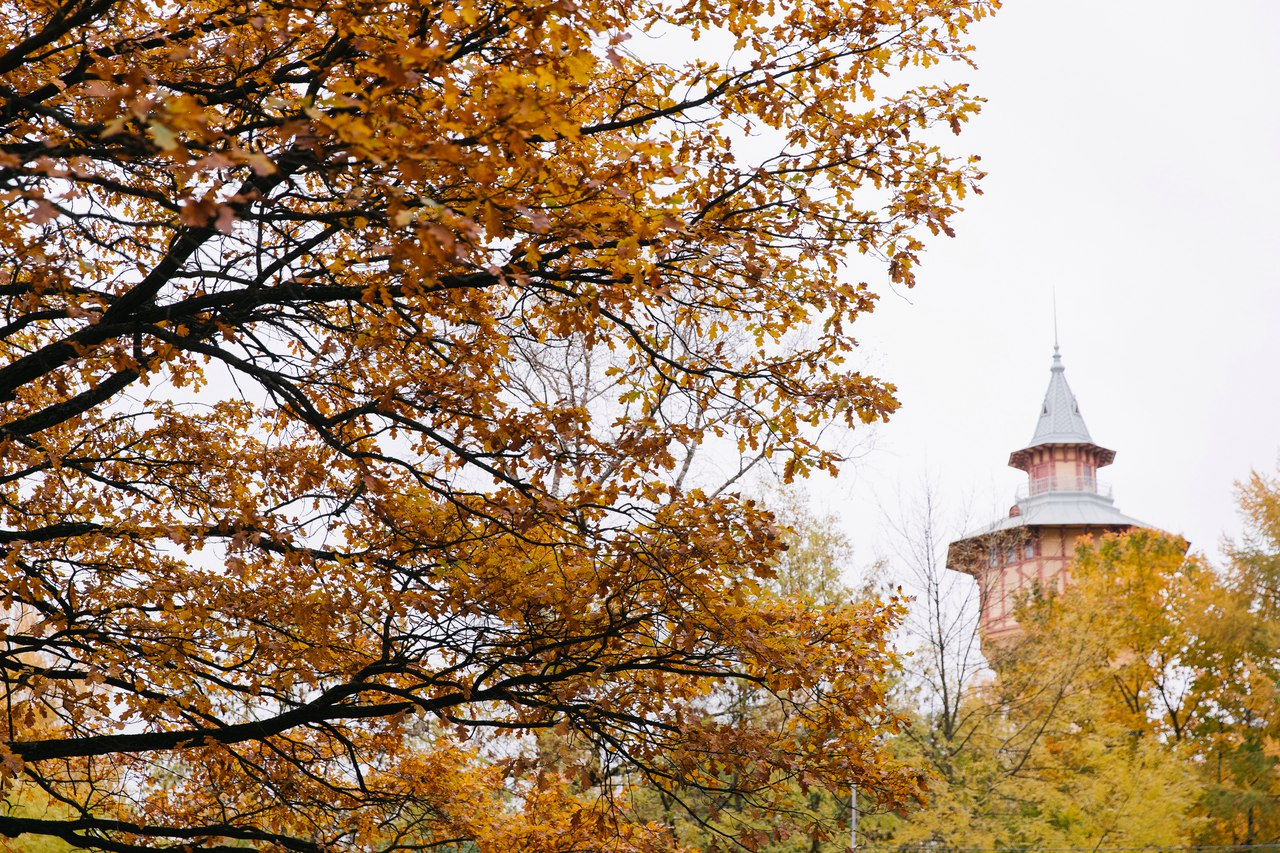
\includegraphics [scale=0.27] {my_folder/images//spbpu_hydrotower}
	\caption{Вид на гидробашню СПбПУ \cite{spbpu-gallery}} 
	\label{fig:spbpu_hydrotower-app2-}  
\end{figure}

\begin{table} [htbp]% Пример оформления таблицы
	\centering\small
	\caption{Представление данных для сквозного примера по ВКР \cite{Peskov2004}}%
	\label{tab:ToyCompare-app2-}		
	\begin{tabular}{|l|l|l|l|l|l|}
		\hline
		$G$&$m_1$&$m_2$&$m_3$&$m_4$&$K$\\
		\hline
		$g_1$&0&1&1&0&1\\ \hline
		$g_2$&1&2&0&1&1\\ \hline
		$g_3$&0&1&0&1&1\\ \hline
		$g_4$&1&2&1&0&2\\ \hline
		$g_5$&1&1&0&1&2\\ \hline
		$g_6$&1&1&1&2&2\\ \hline		
	\end{tabular}	
	\normalsize% возвращаем шрифт к нормальному
\end{table}






\begin{equation}% лучше не оставлять пропущенную строку (\par) перед окружениями для избежания лишних отсупов в pdf
\label{eq:Pi-app2} % eq - equations, далее название, ch поставлено для избежания дублирования
\pi \approx 3,141.
\end{equation}
%
%
\begin{figure}[ht!] 
	\center
	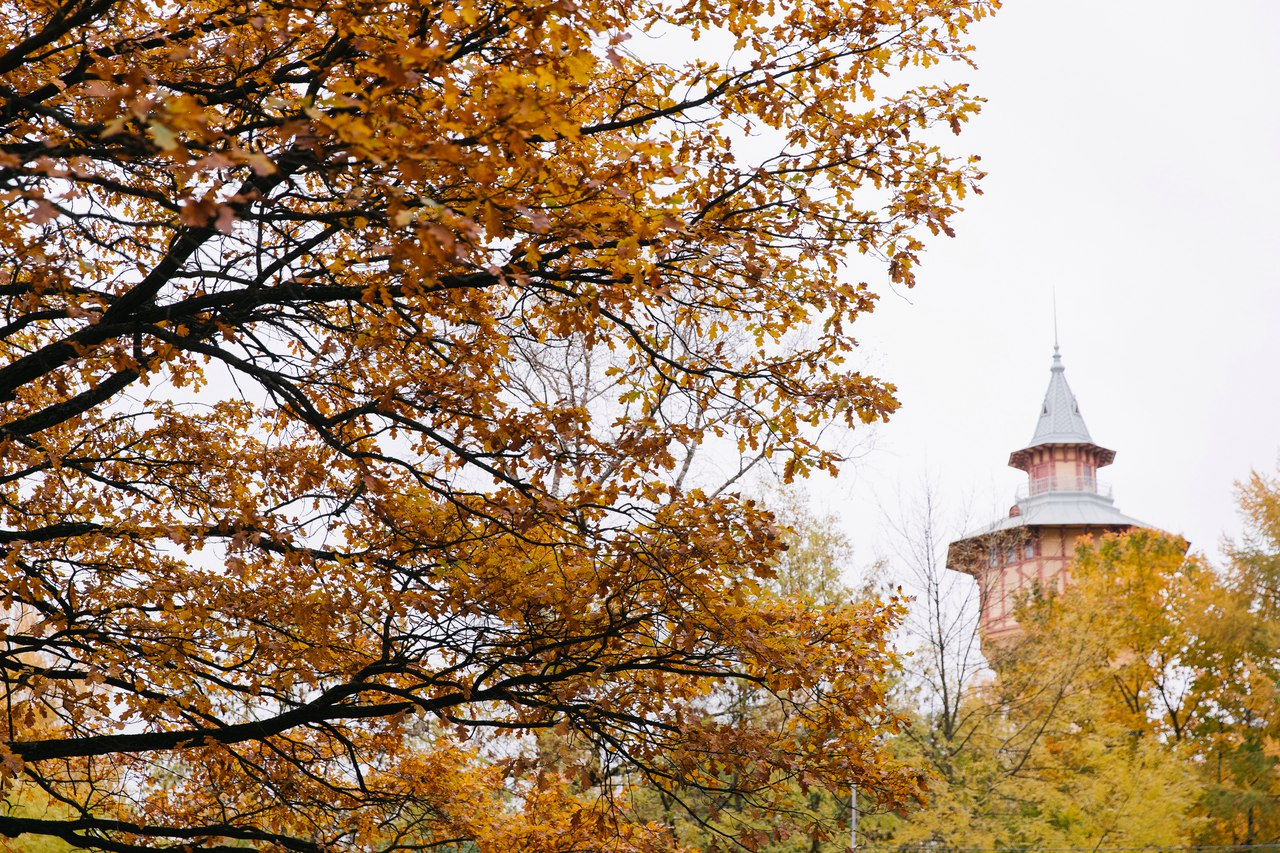
\includegraphics [scale=0.27] {my_folder/images//spbpu_hydrotower}
	\caption{Вид на гидробашню СПбПУ \cite{spbpu-gallery}} 
	\label{fig:spbpu_hydrotower-app2}  
\end{figure}
%




\begin{table}[t!]% Пример оформления таблицы
	\centering\small
	\caption{Представление данных для сквозного примера по ВКР \cite{Peskov2004}}%
	\label{tab:ToyCompare-app2}		
	\begin{tabular}{|l|l|l|l|l|l|}
		\hline
		$G$&$m_1$&$m_2$&$m_3$&$m_4$&$K$\\
		\hline
		$g_1$&0&1&1&0&1\\ \hline
		$g_2$&1&2&0&1&1\\ \hline
		$g_3$&0&1&0&1&1\\ \hline
		$g_4$&1&2&1&0&2\\ \hline
		$g_5$&1&1&0&1&2\\ \hline
		$g_6$&1&1&1&2&2\\ \hline		
	\end{tabular}	
	\normalsize% возвращаем шрифт к нормальному
\end{table}


%% В случае, когда таблица (рисунок) размещаются на последней странице, для переноса названия приложения на новую строку используем:
\NewPage % начать новое приложение с новой страницы 			     % Приложение 1

\chapter{Некоторые дополнительные примеры}\label{appendix-extra-examples}							% 

В приложении\footnote{Внимание! Пример оформления подстрочной ссылки (сноски).} приведены формулы \eqref{eq:Pi-app}, \eqref{eq:Pi-app-}, \firef{fig:spbpu_hydrotower-app}, \firef{fig:spbpu_hydrotower-app-}, \taref{tab:ToyCompare-app}, \taref{tab:ToyCompare-app-}


\begin{equation}% лучше не оставлять пропущенную строку (\par) перед окружениями для избежания лишних отсупов в pdf
\label{eq:Pi-app-} % eq - equations, далее название, ch поставлено для избежания дублирования
\pi \approx 3,141.
\end{equation}
%
%
\begin{figure}[ht!] 
	\center
	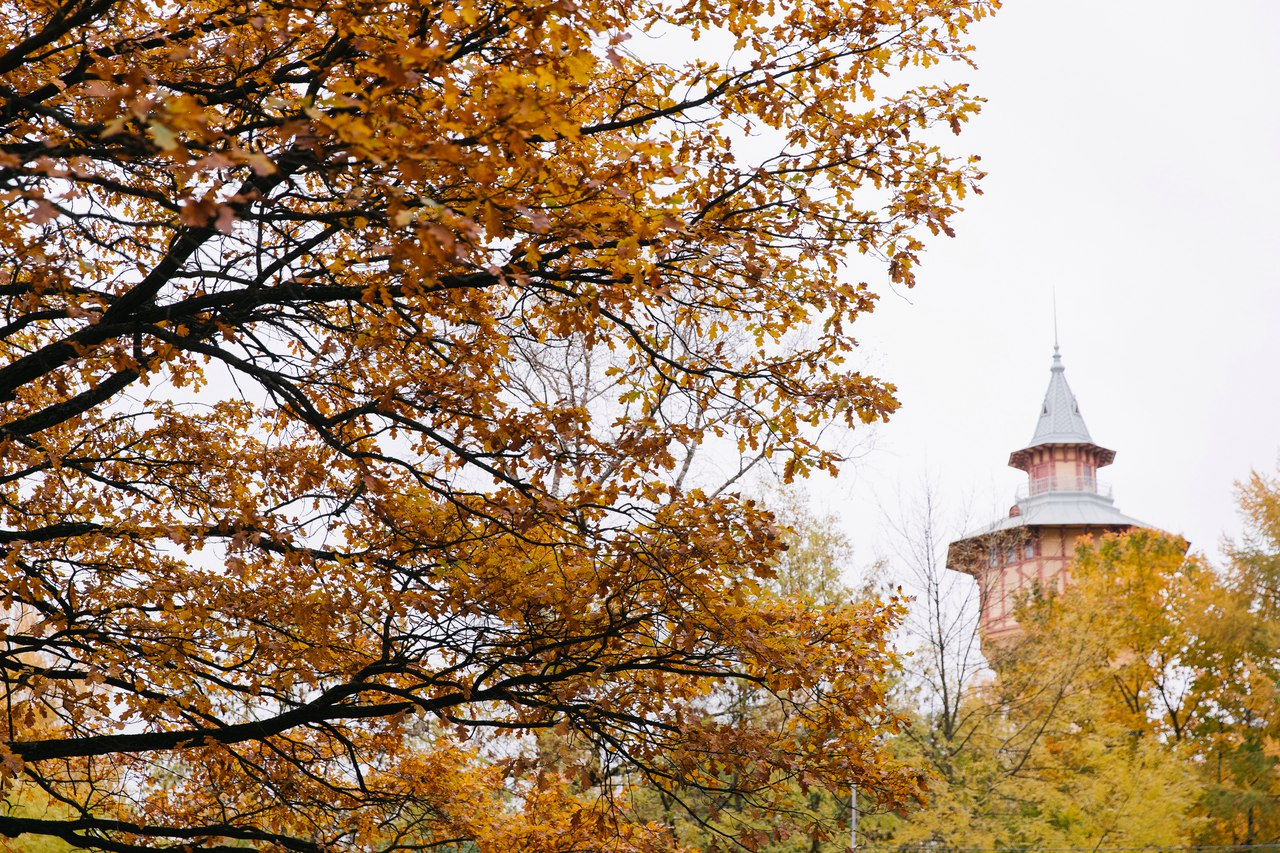
\includegraphics [scale=0.27] {my_folder/images//spbpu_hydrotower}
	\caption{Вид на гидробашню СПбПУ \cite{spbpu-gallery}} 
	\label{fig:spbpu_hydrotower-app-}  
\end{figure}

\begin{table} [htbp]% Пример оформления таблицы
	\centering\small
	\caption{Представление данных для сквозного примера по ВКР \cite{Peskov2004}}%
	\label{tab:ToyCompare-app-}		
	\begin{tabular}{|l|l|l|l|l|l|}
		\hline
		$G$&$m_1$&$m_2$&$m_3$&$m_4$&$K$\\
		\hline
		$g_1$&0&1&1&0&1\\ \hline
		$g_2$&1&2&0&1&1\\ \hline
		$g_3$&0&1&0&1&1\\ \hline
		$g_4$&1&2&1&0&2\\ \hline
		$g_5$&1&1&0&1&2\\ \hline
		$g_6$&1&1&1&2&2\\ \hline		
	\end{tabular}	
	\normalsize% возвращаем шрифт к нормальному
\end{table}



						


\begin{equation}% лучше не оставлять пропущенную строку (\par) перед окружениями для избежания лишних отсупов в pdf
\label{eq:Pi-app} % eq - equations, далее название, ch поставлено для избежания дублирования
\pi \approx 3,141.
\end{equation}
%
%
\begin{figure}[ht!] 
	\center
	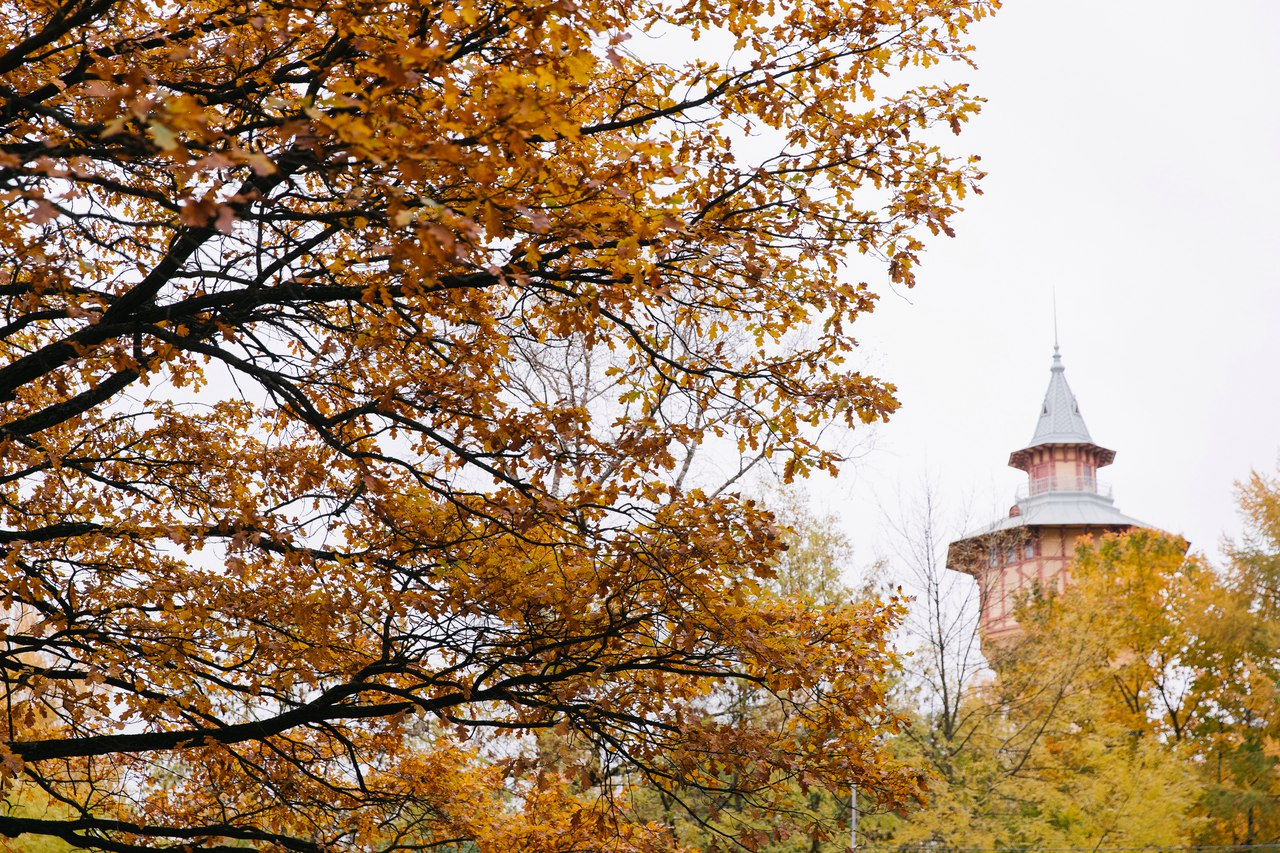
\includegraphics [scale=0.27] {my_folder/images//spbpu_hydrotower}
	\caption{Вид на гидробашню СПбПУ \cite{spbpu-gallery}} 
	\label{fig:spbpu_hydrotower-app}  
\end{figure}

\begin{table} [htbp]% Пример оформления таблицы
	\centering\small
	\caption{Представление данных для сквозного примера по ВКР \cite{Peskov2004}}%
	\label{tab:ToyCompare-app}		
	\begin{tabular}{|l|l|l|l|l|l|}
		\hline
		$G$&$m_1$&$m_2$&$m_3$&$m_4$&$K$\\
		\hline
		$g_1$&0&1&1&0&1\\ \hline
		$g_2$&1&2&0&1&1\\ \hline
		$g_3$&0&1&0&1&1\\ \hline
		$g_4$&1&2&1&0&2\\ \hline
		$g_5$&1&1&0&1&2\\ \hline
		$g_6$&1&1&1&2&2\\ \hline		
	\end{tabular}	
	\normalsize% возвращаем шрифт к нормальному
\end{table}

			 	 % Приложение 2


\end{document} % конец документа


%%% Удачной защиты ВКР! - Good luck on the thesis defense!
%%
%%% Поддержать проект
%%
%% Запросы на добавление / изменение просим писать на следующей странице:
%% https://github.com/ParkhomenkoV/SPbPU-student-thesis-template/issues
%%
%% Список пожеланий в файле шаблона <<TO-DO-list.tex>>
%%
%% Благодарности просим указывать в виде 
%%
%% 1. Добавление <<Звезды>> проекту https://github.com/ParkhomenkoV/SPbPU-student-thesis-template/stargazers
%%
%% 2. Добавления <<Сердечка>> и репоста проекта в социальных сетях:
%%		https://vk.com/latex_polytech 
%%		https://www.fb.com/groups/latex.polytech
%%

%%% Support project
%%
%% Requests on adding / modifications is better to be publishen on the following web-page:
%% https://github.com/ParkhomenkoV/SPbPU-student-thesis-template/issues
%%
%% Wishlist is in the template's file called <<TO-DO-list.tex>>
%%
%% Acknowledgements are better to be done in the form of 
%%
%% 1. Adding <<Star>> to the project https://github.com/ParkhomenkoV/SPbPU-student-thesis-template/stargazers
%%
%% 2. Adding <<Likes>> and Project repost in the social networks:
%%		https://vk.com/latex_polytech 
%%		https://www.fb.com/groups/latex.polytech
%% 

% Check list при передаче ВКР:
% - Количество страниц в Задании 2. Если нет, то комментирование последней строки в my_task.tex
% - Зачистка всех вспомогательных файлов (Clear auxilary files) и компиляция ВКР не менее 3х раз